%%%%%%%% ICML 2025 EXAMPLE LATEX SUBMISSION FILE %%%%%%%%%%%%%%%%%

\documentclass{article}

% Recommended, but optional, packages for figures and better typesetting:
\usepackage{microtype}
\usepackage{graphicx}
\usepackage{subfigure}
\usepackage{booktabs} % for professional tables
\usepackage{multirow}
\usepackage{bm}
\usepackage{xcolor}
\usepackage{amsmath}
\usepackage{amsthm}
% \usepackage{subcaption}
% \newcommand{\changed}[1]{\textcolor{blue}{#1}}
% \newcommand{\todo}[1]{\textcolor{red}{#1}}
\newtheorem{hypothesis}{Hypothesis}
\usepackage{caption}
\usepackage{float} 
%\usepackage{subfigure}
% \usepackage{subcaption}
\usepackage{amsmath,amssymb,amsfonts}
\usepackage{algorithmic}
\usepackage{textcomp}
\usepackage{bm}
\usepackage{amsfonts}
\usepackage{xcolor}
\usepackage{diagbox}
\usepackage{booktabs}
\usepackage[normalem]{ulem}
\usepackage{multirow}
\usepackage{pifont}
\usepackage{enumitem}

% \usepackage[linesnumbered,ruled,vlined]{algorithm2e}
\usepackage[ruled,vlined]{algorithm2e}
\usepackage{amsmath}
\usepackage{graphicx}

\newcommand{\cmark}{\textcolor{green!50!black}{\ding{51}}}
\newcommand{\xmark}{\textcolor{red}{\ding{55}}}
\newcommand{\neutral}{\textcolor{blue!50!white}{\ding{108}}}

% hyperref makes hyperlinks in the resulting PDF.
% If your build breaks (sometimes temporarily if a hyperlink spans a page)
% please comment out the following usepackage line and replace
% \usepackage{icml2025} with \usepackage[nohyperref]{icml2025} above.
\usepackage{hyperref}


% Attempt to make hyperref and algorithmic work together better:
\newcommand{\theHalgorithm}{\arabic{algorithm}}

% Use the following line for the initial blind version submitted for review:
% \usepackage{icml2025}

% If accepted, instead use the following line for the camera-ready submission:
\usepackage[accepted]{icml2025}

% For theorems and such
\usepackage{amsmath}
\usepackage{amssymb}
\usepackage{mathtools}
\usepackage{amsthm}
\usepackage{colortbl}
\usepackage{tikz}      % 用于绘制图形
\usepackage{colortbl}
\usepackage{float}
\usepackage{listings}
\lstset{
    language=Python,              % 设置语言为 Python
    basicstyle=\rmfamily\small,   % 基础字体样式
    keywordstyle=\color{red},    % 关键词颜色
    commentstyle=\color{green!50!black},    % 注释颜色
    frame=single,                 % 添加边框
    breaklines=true,              % 自动换行
    tabsize=4                     % Tab 键大小
}

% \definecolor{background}{RGB}{245,245,245} % 背景色
% \definecolor{keyword}{RGB}{183,72,182}     % 关键词颜色
% \definecolor{string}{RGB}{196,26,22}       % 字符串颜色
% \definecolor{comment}{RGB}{0,128,0}        % 注释颜色
% \definecolor{variable}{RGB}{51,51,255}     % 变量颜色
% \definecolor{number}{RGB}{170,13,145}      % 数字颜色

% % 自定义minted样式
% \lstset{
%     language=Python,
%     bgcolor=background,          % 背景色
%     frame=lines,                 % 边框
%     framesep=2mm,                % 边框和内容间距
%     linenos,                     % 显示行号
%     numbersep=5pt,               % 行号间距
%     fontfamily=tt,               % 等宽字体
%     fontsize=\small,             % 字体大小
%     xleftmargin=10pt,            % 左边距
%     breaklines=true,             % 自动换行
%     tabsize=4,                   % Tab 大小
%     keywordstyle=\color{keyword},% 关键词颜色
%     stringstyle=\color{string},  % 字符串颜色
%     commentstyle=\color{comment},% 注释颜色
%     numberstyle=\tiny\color{gray}, % 行号样式
% }

% if you use cleveref..
\usepackage[capitalize,noabbrev]{cleveref}

%%%%%%%%%%%%%%%%%%%%%%%%%%%%%%%%
% THEOREMS
%%%%%%%%%%%%%%%%%%%%%%%%%%%%%%%%
\theoremstyle{plain}
\newtheorem{theorem}{Theorem}[section]
\newtheorem{proposition}[theorem]{Proposition}
\newtheorem{lemma}[theorem]{Lemma}
\newtheorem{corollary}[theorem]{Corollary}
\theoremstyle{definition}
\newtheorem{definition}[theorem]{Definition}
\newtheorem{assumption}[theorem]{Assumption}
\theoremstyle{remark}
\newtheorem{remark}[theorem]{Remark}
% \usepackage{ulem}

% Todonotes is useful during development; simply uncomment the next line
%    and comment out the line below the next line to turn off comments
%\usepackage[disable,textsize=tiny]{todonotes}
\usepackage[textsize=tiny]{todonotes}


% The \icmltitle you define below is probably too long as a header.
% Therefore, a short form for the running title is supplied here:
\icmltitlerunning{}


\begin{document}

\twocolumn[
\icmltitle{Harmony in Divergence: Towards Fast, Accurate, and Memory-efficient Zeroth-order LLM Fine-tuning}

% It is OKAY to include author information, even for blind
% submissions: the style file will automatically remove it for you
% unless you've provided the [accepted] option to the icml2025
% package.

% List of affiliations: The first argument should be a (short)
% identifier you will use later to specify author affiliations
% Academic affiliations should list Department, University, City, Region, Country
% Industry affiliations should list Company, City, Region, Country

% You can specify symbols, otherwise they are numbered in order.
% Ideally, you should not use this facility. Affiliations will be numbered
% in order of appearance and this is the preferred way.
\icmlsetsymbol{equal}{*}

\begin{icmlauthorlist}
\icmlauthor{Qitao Tan}{uga}
\icmlauthor{Jun Liu}{neu}
\icmlauthor{Zheng Zhan}{neu}
\icmlauthor{Caiwen Ding}{umt}
\icmlauthor{Yanzhi Wang}{neu}
\icmlauthor{Jin Lu}{uga}
\icmlauthor{Geng Yuan}{uga}
\end{icmlauthorlist}

\icmlaffiliation{uga}{University of Georgia}
\icmlaffiliation{neu}{Northeastern University}
\icmlaffiliation{umt}{University of Minnesota Twin Cities}

\icmlcorrespondingauthor{Geng Yuan}{geng.yuan@uga.edu}
% \icmlcorrespondingauthor{Firstname2 Lastname2}{first2.last2@www.uk}

% You may provide any keywords that you
% find helpful for describing your paper; these are used to populate
% the "keywords" metadata in the PDF but will not be shown in the document
\icmlkeywords{Machine Learning, ICML}

\vskip 0.3in
]

% this must go after the closing bracket ] following \twocolumn[ ...

% This command actually creates the footnote in the first column
% listing the affiliations and the copyright notice.
% The command takes one argument, which is text to display at the start of the footnote.
% The \icmlEqualContribution command is standard text for equal contribution.
% Remove it (just {}) if you do not need this facility.

%\printAffiliationsAndNotice{}  % leave blank if no need to mention equal contribution
\printAffiliationsAndNotice{\icmlEqualContribution} % otherwise use the standard text.


\begin{abstract}
% Large language models (LLMs) demonstrate exceptional performance across a variety of tasks, yet standard first-order (FO) fine-tuning requires considerable memory, significantly limiting practical deployment. 
% Recently, zeroth-order (ZO) optimization stood out as a promising memory-saving training paradigm, foregoing memory-intensive backward passes and estimating gradients solely through forward passes, offering an attractive solution for resource-constrained scenarios. 
Large language models (LLMs) excel across various tasks, but standard first-order (FO) fine-tuning demands considerable memory, significantly limiting real-world deployment. Recently, zeroth-order (ZO) optimization stood out as a promising memory-efficient training paradigm, avoiding backward passes and relying solely on forward passes for gradient estimation, making it attractive for resource-constrained scenarios. However, ZO method lags far behind FO method in both convergence speed and accuracy. To bridge the gap, we introduce a novel layer-wise divergence analysis that uncovers the distinct update pattern of FO and ZO optimization. Aiming to resemble the learning capacity of FO method from the findings, we propose \textbf{Di}vergence-driven \textbf{Z}eroth-\textbf{O}rder (\textbf{DiZO}) optimization. DiZO conducts divergence-driven layer adaptation by incorporating projections to ZO updates, generating diverse-magnitude updates precisely scaled to layer-wise individual optimization needs. Our results demonstrate that DiZO significantly reduces the needed iterations for convergence without sacrificing throughput, cutting training GPU hours by up to 48\% on various datasets. Moreover, DiZO consistently outperforms the representative ZO baselines in fine-tuning RoBERTa-large, OPT-series, and Llama-series on downstream tasks and, in some cases, even surpasses memory-intensive FO fine-tuning.
% Large language models (LLMs) excel in many tasks, but the memory-intensive first-order (FO) fine-tuning greatly limits real-world deployment. In contrast, zeroth-order (ZO) optimization, a promising approach that estimates gradients using only forward passes, significantly reduces memory burden, making it an attractive solution for memory-constrained applications. However, an obvious accuracy and convergence speed gap still exists between these methods and the FO methods. In this work, we first introduce a novel distance-based analysis to investigate the difference in training dynamics between FO and ZO. Aiming to resemble the learning capacity of FO from the findings, we propose \textbf{P}rojection-\textbf{e}nhanced \textbf{Z}eroth-\textbf{O}rder (\textbf{PeZO}) optimization. PeZO conducts projection to the updates from ZO steps, generating customized updates precisely scaled to layer-wise individual optimization needs. Our results demonstrate that PeZO significantly reduces the needed iterations for convergence, cutting GPU hours by up to 48\% on a broad range of datasets, all without sacrificing throughput. Moreover, PeZO consistently outperforms the representative ZO method in fine-tuning RoBERTa, OPT, and Llama on various downstream tasks, achieving superior accuracy.
\end{abstract}

\section{Introduction}



Fine-tuning pre-trained large language models (LLMs) with backpropagation demonstrates
superior performance for many natural language processing tasks~\cite{yang2019end, liu2019roberta,talmor2018commonsenseqa,chowdhery2023palm,zheng2020end}. However, the extensive parameterization imposes a substantial memory burden, limiting their practicality for widespread downstream applications.
% Fine-tuning pre-trained large language models (LLMs) is the state-of-the-art approach for many natural language processing tasks. However, the extensive parameterization and high computational costs have become significant constraints in wide applications. 
In line with the neural scaling laws~\cite{hoffmann2022empirical,kaplan2020scaling}, next-generation LLMs continue to increase in parameter count. Specifically, model sizes are expanding at a rate of 410× every two years, dramatically outpacing the scaling of DRAM bandwidth (1.4× every two years) and DRAM capacity (2× every two years). This disparity leads to the \emph{memory wall} challenge~\cite{gholami2024ai}, which becomes even more severe when deploying LLMs on memory-limited devices~\cite{zeng2024flightllm,chen2024understanding,hur2023fast}.

Recently, zeroth-order (ZO) optimization has emerged as a promising memory-efficient training paradigm for LLM fine-tuning, attracting significant attention~\cite{zhang2024revisiting,liu2024sparse,malladi2023fine, zhao2024second}.
By relying solely on forward passes (i.e., inference) to estimate gradients and update model parameters, ZO bypasses the need for backward propagation and significantly reduces extensive storage requirements for activations, gradients, and optimizer states.
% This method intends only to use forward passes (i.e., inference) to estimate the gradients and update the weights accordingly.
% By completely avoiding the computation of backward propagation, ZO simplifies the computation process and eliminates the need for storing extensive data, including activations, gradients, and optimizer state. 
As reported in~\citet{malladi2023fine}, fine-tuning LLMs via ZO optimization reduces up to 12$\times$ memory cost.
Nevertheless, ZO optimization still exhibits a \textbf{gap} in convergence speed and accuracy compared to the conventional first-order (FO) method (i.e., compute gradient via backpropagation). As shown in Table~\ref{table1}, one can observe that the FO method substantially outperforms ZO method in both accuracy and GPU hours. Though ZO method achieves higher throughput due to its computational simplicity, it requires more than 10× iterations for convergence, dramatically increasing GPU hours. Previous studies typically attribute this gap to the fact that ZO optimization leverages random perturbation for gradient estimation, and thus results in unavoidable estimation error, but without further exploration of other underlying causes~\cite{malladi2023fine, gautam2024variance, zhao2024second}. 


% \begin{table}[t]
% \centering
% \scalebox{0.78}{
% \begin{tabular}{lccccc}
% \toprule
% Model                      & \textbf{Type} & \textbf{Acc} & \textbf{Throughput} & \textbf{Iteration} & \textbf{GPU hours} \\ \hline
% \multirow{2}{*}{RoBERTa-L} & FO   & 91.9 & 2.32 it/s  & 6.6\%     & 12.3\%    \\
%                            & ZO   & 90.5 & 5.12 it/s  & 100.0\%     & 100.0\%     \\ \hline \hline
% \multirow{2}{*}{OPT-2.7B}  & FO   & 94.2 & 1.81 it/s  & 7.5\%     & 16.8\%    \\
%                            & ZO   & 90.0 & 3.28 it/s  & 100.0\%     & 100.0\%     \\
% \bottomrule
% \end{tabular}
% }
% \caption{Fine-tuning results on SST-2 datasets. FO outperforms the ZO method in terms of both accuracy and GPU hours.}
% \label{table1}
% \end{table}

% To fill up the identified capacity gap, we begin by analyzing the distinct optimization patterns exhibited by ZO and FO methods in LLM fine-tuning. Our analysis reveals that ZO and FO present notably different training dynamics, reflected by the layer-wise distance between the pre-trained model and the fine-tuned model. Specifically, FO benefits from more accurate gradient estimates, it applies \underline{layer-wise customized updates} according to layer-wise individual optimization needs. In contrast, due to the high-dimensional random search inherent nature of ZO, it applies \underline{layer-wise uniform-magnitude updates}. Motivated by these observations, we are interested in investigating: \emph{if we can also provide ZO with layer-wise customized updates, effectively accelerating the training and enhancing performance.} 
To bridge this gap, we begin by examining the distinct update patterns shown by ZO and FO methods during LLM fine-tuning. Our analysis reveals a substantial difference in their layer-wise update magnitudes. Specifically, ZO method relies on high-dimensional random search and tends to apply \underline{uniform-magnitude updates} without considering layer-wise individual characteristics. In contrast, FO method benefits from fine-grained gradient estimation and applies \underline{diverse-magnitude updates} precisely scaled to the layer-wise individual optimization needs.
Motivated by these observations, we are interested in investigating: \emph{if we can also provide ZO with diverse-magnitude updates, effectively achieving training acceleration and accuracy improvement. }
% as indicated by the variance of layer-wise weight distance gaps between the pre-trained and fine-tuned model. Specifically, ZO optimization, due to its reliance on high-dimensional random search, applies uniform-magnitude updates across all layers without considering individual layer characteristics.   \emph{if we can also provide ZO with layer-wise customized updates, effectively accelerating the training and enhancing performance.}


% To pinpoint the reasons for the gap, we begin by analyzing the distinct training dynamics exhibited by ZO and FO methods in LLM fine-tuning. Our analysis reveals that ZO and FO present notably different layer-wise divergence, reflected by the distance between the pre-trained model and the fine-tuned model. Specifically, FO benefits from more accurate gradient estimation, ensuring each layer receives updates precisely scaled to its individual optimization needs. In contrast, due to the inherent nature of high-dimensional random search, ZO applies non-careful uniform-magnitude updates across layers. Motivated by these observations, we are interested in investigating: \emph{if we can also provide ZO with layer-wise customized updates, effectively accelerating the training and enhancing performance.} 

Drawing on these insights, we propose \textbf{Di}vergence-driven \textbf{Z}eroth-\textbf{O}rder optimization (\textbf{DiZO}). DiZO conducts divergence-driven layer adaptation by incorporating projections, enabling layer-wise adaptive updates that closely resemble FO approaches. Notably, the projections can be optimized without gradients, ensuring that DiZO retains the appealing backpropagation-free features. Moreover, we validate DiZO on a variety of tasks, including classification and generation, using several LLMs such as RoBERTa-large, the OPT series, and the Llama series. Experimental results show that DiZO substantially decreases training iterations for convergence while maintaining throughput, cutting training GPU hours by up to 48\% on diverse datasets. Furthermore, our method can be seamlessly integrated with parameter-efficient tuning techniques like low-rank adaptation~\cite{hu2021lora} for additional speedups. DiZO also consistently outperforms the representative ZO baselines and, in some cases, surpasses memory-intensive FO fine-tuning. 
% \todo{add lora}
% 举个例子,4090 fine-tuning 2.7B, FO装不下,MeZO比较慢

% (某些数据集好于fine-tune,mezo不行) 
% Moreover, by substantially reducing the number of iterations required for convergence and without compromising throughput, PeZO cuts GPU hours by up to 50\% compared to vanilla ZO.

% accelerates convergence by up to 50\% relative to vanilla ZO, substantially reducing the number of training steps required.
% up to 50\% acceleration compared with the vanilla ZO. Moreover, an average 1.5\% accuracy increase is obtained over classification and 2.5\& perplexity increase over generation.

% We found that the slow optimization of ZO is not only due to the inappropriate optimization direction caused by its random search nature but also due to the inappropriate parameter update magnitude of each training step. In detail, the update magnitude of ZO depends on three terms, learning rate, finite difference of the target function, and the magnitude of the random sampled perturbation. The first two terms are the same for all network layers in one single step, however, the last term, due to the dimensional curse, when optimizing high-dimensioned LLM, is also the same for all layers, resulting in all layers and parameters having similar step magnitude. In contrast, the FO method provides distinguishing step magnitude and quickly accumulates layer-wise difference thus having better convergence speed and performance. We summarize the above finding and propose a hypothesis in Section~\ref{hypo}.
% propose the following hypothesis (details in \ref{hypo}): \textbf{\emph{layers of LLM prefer different magnitude gaps with the pre-trained model, ZO needs to take many more steps to accumulate such gaps}}. 


The summary of our contributions is as follows:
\begin{itemize}
    \item We introduce a novel layer-wise divergence analysis to uncover the fundamental differences in the updating patterns of FO and ZO methods.
    \item We introduce DiZO, a novel ZO method using divergence-driven layer adaptation,
    achieving a learning capacity closely resembling FO while maintaining the throughput benefit of ZO optimization.
    \item DiZO consistently exceeds existing baselines in both accuracy and GPU hours, and it can be seamlessly integrated with LoRA for additional benefits. These advantages hold across diverse tasks and LLM architectures.
\end{itemize}


% Please add the following required packages to your document preamble:
% \usepackage{multirow}


% Despite the advantages taken by ZO optimization, it faces the dilemma of slow convergence speed. As shown in~\ref{table1}, ZO achieves higher throughput due to its computational simplicity, but it also takes 20× training steps for convergence and finally results in 10× GPU hours. We attribute the slow convergence to the indiscriminate sampled perturbations for each layer. As shown in Figure~\ref{figure1}, both in FO or ZO, different layers have their different magnitude gap with the pre-trained model (Figure~\ref{figure1} left). However, in ZO optimization, since all layers are perturbed by randomly sampled high-dimensioned random vectors, each of them is perturbed to have a similar magnitude gap with the pre-trained model. Thus, ZO optimization needs to accumulate the gap to achieve the discriminate magnitude gap preferred by each layer, and that is why ZO optimization needs many more steps for convergence compared with the FO method. Based on the above observation, we state the following hypothesis.

\begin{figure*}[ht]
\centering
% \includegraphics[width=1\linewidth]{icml2025/texs/figures/ZOFO_illustration.pdf}
\scalebox{0.95}{
\includegraphics[width=1\linewidth]{FOZO_illustration_new.pdf}
}
\caption{Comparison of the training dynamics of ZO and FO methods. The X-axis represents layer names, and the Y-axis represents the distance gap. Although they converge to different stable states, the divergence of the distance gap increases in both FO and ZO methods during training. FO accumulates divergence rapidly through diverse-magnitude updates, while ZO applies uniform-magnitude updates, requiring more iterations for an ideal divergence level. Results are obtained by fine-tuning OPT-2.7B on the SST-2 dataset, focusing on weights in the attention module: K (Key), V (Value), Q (Query), and O (Output projection). }

\label{zo_fo}
\end{figure*}
\section{Preliminaries and Pattern Analysis}


\subsection{Revisiting Zeroth-order Optimization}
Recently, ZO optimization has gained significant attention in machine learning~\cite{verma2023certified,dhurandhar2019model,wang2022zarts,gu2021efficient}.
Unlike conventional FO optimization, which calculates gradients via backpropagation, ZO optimization estimates gradients using only objective oracles via finite differences \cite{chen2023deepzero, liu2018zeroth, ye2018hessian}. This property can be leveraged for LLM fine-tuning to alleviate the extensive memory costs. Specifically, as ZO only needs two forward passes to obtain the estimated gradients, it avoids computing and storing the most memory-consuming information needed in the conventional FO training, i.e., activations in the forward process, gradients in the backward process, and the optimizer state.
% MeZO~\cite{malladi2023fine} introduced a ZO-SGD algorithm for fine-tuning LMs, reducing memory usage by up to 12× without compromising accuracy. 
% Building on this, \cite{liu2024sparse} applied sparse techniques to MeZO, optimizing only a subset of parameters for faster training without performance loss. \cite{tang2024private} proposed a differentially private ZO method for privacy-preserving fine-tuning, while \cite{ling2024convergence} integrated ZO into federated learning to support memory-constrained clients.

The core idea of ZO optimization is to estimate gradients by applying random perturbations to the weights and computing differences in the objective. For a mini-batch of data $\mathcal{B}$, sampled from a labeled dataset $\mathcal{D} = \{x_{i}, y_{i}\}_{i=1}^{|\mathcal{D}|}$, a model with parameters $\bm{\theta} \in \mathbb{R}^{d}$, where $d$ represents the dimension of the parameter space, and the corresponding loss function $\mathcal{L}(\bm{\theta}; \mathcal{B})$. The gradient is estimated as follows:
\begin{equation}
\label{equ:1}
    \nabla \mathcal{L}(\bm{\theta};\mathcal{B})=\frac{1}{q} \sum_{i=1}^q\left[\frac{\mathcal{L}\left(\bm{\theta}+\epsilon \bm{u}_{i};\mathcal{B}\right)-\mathcal{L}\left(\bm{\theta}-\epsilon \bm{u}_{i};\mathcal{B}\right)}{2 \epsilon} \bm{u}_{i}\right]
\end{equation}
where $\bm{u}_{i}$ is a random vector with the same dimension as the model weights and is typically drawn from standard Gaussian distribution $\mathcal{N}(0, \mathbf{I})$~\cite{malladi2023fine, zhang2024revisiting}, or from Gaussian
sampling over a unit sphere~\cite{liu2018zeroth, shamir2017optimal}, $q$ is the number of objective queries, and $\epsilon > 0$ is a small perturbation scalar for smoothing.
\begin{table}[t]
\centering
\caption{Fine-tuning results on SST-2 datasets. Although ZO method shows advantages in memory saving, left behind FO method in terms of both accuracy and GPU hours.
% \red{Move to page 2 top-right}
}
\vspace{5pt}
\scalebox{0.93}{

\begin{tabular}{lccccc}
\toprule
Model                     & \textbf{Type} & \textbf{Acc.} & \textbf{Memory} & \textbf{\begin{tabular}[c]{@{}c@{}}\#Train\\ Iter.\end{tabular}} & \textbf{\begin{tabular}[c]{@{}c@{}}GPU \\ Hours\end{tabular}} \\ \hline
\multirow{2}{*}{RoBERTa}  & FO            & 91.9         & 9.2 GB          & 6.6\%                                                          & 12.3\%                                                        \\
                          & ZO            & 90.5         & 4.5 GB          & 100.0\%                                                        & 100.0\%                                                       \\ \hline \hline
\multirow{2}{*}{OPT-2.7B} & FO            & 94.2         & 45.4 GB         & 7.5\%                                                          & 16.8\%                                                        \\
                          & ZO            & 90.0         & 6.8 GB          & 100.0\%                                                        & 100.0\%                                                       \\ \bottomrule
\end{tabular}
}
\vspace{-10pt}
\label{table1}
\end{table}

Given the learning rate $\eta$ and the mini-batch data $\mathcal{B}_{t}$ at $t$-th iteration, once the estimated gradient $\nabla \mathcal{L} (\theta;\mathcal{B}_{t})$ is obtained,
then ZO-SGD updates the parameters with the following rule:
\begin{equation}
\label{equ:2}
    \bm{\theta}_{t+1} = \bm{\theta}_{t} - \eta \nabla \mathcal{L}(\bm{\theta}_{t};\mathcal{B}_{t})
\end{equation}


\subsection{Layer-wise Divergence Analysis}
\label{hypo}
Drawing insight from the update formula of ZO optimization, we notice that ZO method applies uniform-magnitude updates across layers, e.g., the L2-norm of the updates is about the same for all layers in one iteration (see Appendix~\ref{proof} for proof). This fact may be the root of the inferior performance of ZO optimization. To measure how the divergence of update magnitude affects the convergence speed and accuracy, we investigate the training dynamics of ZO and FO methods, respectively.
% To better understand the difference of layer-wise update magnitudes between FO and ZO methods and assess the impact of these differences on training, we analyze their training dynamics respectively.

% Drawing insight from the update formula of ZO optimization, we notice that ZO applies uniform-magnitude updates across layers, e.g., the L2-norm of the updates is about the same for all layers in one iteration (see Appendix~\ref{proof} for proof). This characteristic may be the root of the performance gap between the FO and ZO methods. To this end, aiming to understand the differences in their update patterns further, we explore the divergence of layer-wise update magnitude and its impact on fine-tuning convergence speed and accuracy in the ZO and FO methods, respectively. 
% in the fine-tuning process using FO and ZO, respectively. 
% For simplicity, in the following sections, we use layer-wise divergence to refer to the divergence of layer-wise update magnitude.

% Previous studies on ZO optimization suggest that the convergence speed is related to the variance of estimated gradients, lower variance will result in faster convergence, thus, many ZO acceleration methods have been proposed around variance reduction~\cite{liu2018zeroth, ji2019improved, sener2020learning, sarafian2020explicit, maheswaranathan2019guided}. However, they rather focus on small-scale optimization problems or aim to reduce the number of the function queries (already proofed one is enough in LLM ZO optimization~\cite{malladi2023fine}), while there is little research trying to accelerate ZO LLM fine-tuning from the perspective of training dynamics. 

% For simplicity, in the following sections, we use layer-wise divergence to refer to the divergence of layer-wise update magnitude.

% of the fine-tuned model under both FO and ZO, 
% In the rest of the paper, we refer to it as layer-wise divergence in short.

% Previous works studying the training dynamics of ZO optimization, we investigate the distance between the fine-tuned model and the pre-trained model.}

% We define distance as ...., and we define distance gap

\textbf{Analysis indicator.} To quantify the effect of updates, we adapt the layer-wise L2-norm distance gap between the weights of the pre-trained and the fine-tuned model as an indicator.
The layer-wise L2-norm distance gap is defined as:
\begin{equation}
    \|\Delta \bm{\theta}_{t}^{(\ell)}\| = \|\bm{\theta}_{t}^{(\ell)} - \bm{\theta}_{0}^{(\ell)}\|_2
\end{equation}
where $t$ is $t$-th fine-tuning iteration, $\ell$ is $\ell$-th layer of the model, and $\bm{\theta}_{0}^{(\ell)}$ indicates the weights of $\ell$-th layer of pre-trained model. 

% \textbf{Analysis metric.} To quantify the layer-wise divergence, we adapt the layer-wise L2-norm distance gap between the weights of the pre-trained and the fine-tuned model as an indicator. Intuitively, if each layer undergoes diverse update magnitudes, its distance from the pre-trained model will also be diverse accordingly.
% % Our intuition is that if the layer-wise update magnitude is diverse, then the distance gap of each layer is also supposed to be diverse.  
% % There are distance gaps for layers, the larger the variance of the gaps, the larger the divergence, and vice versa. For example, 
% The layer-wise L2-norm distance gap is defined as:
% \begin{equation}
%     \|\Delta \bm{\theta}_{t}^{(\ell)}\| = \|\bm{\theta}_{t}^{(\ell)} - \bm{\theta}_{0}^{(\ell)}\|_2
% \end{equation}
% where $t$ is $t$-th fine-tuning iteration, $\ell$ is $\ell$-th layer of the model, and $\bm{\theta}_{0}^{(\ell)}$ indicates the $\ell$-th layer of pre-trained model. 
% The larger the variance of distance of layers, the higher the divergence of the layers.
% the layer-wise divergence increases over the fine-tuning process and ultimately converges to a stable state, suggesting that different layers profit from maintaining diverse distance gaps with the pre-trained model

% \textbf{Analysis result.} Figure~\ref{zo_fo} compares the training dynamics of FO and ZO methods. As one can observe, regardless of ZO or FO, the divergence of the distance gap increases during training, i.e., the line of distance gap gradually 'bends', suggesting that different layers profit from maintaining diverse gaps with the pre-trained model. However, FO and ZO differ in how the distance gap divergence is accumulated. FO employs fine-grained gradient estimations, resulting in diverse-magnitude updates (FO updates in Figure~\ref{zo_fo}). Therefore, it can rapidly reach the desired layer-wise distance gap in only a few iterations. In contrast, ZO relies on random search in high-dimensional parameter space and generates uniform-magnitude updates (ZO updates in Figure~\ref{zo_fo}), resulting in thousands more iterations required for accumulating a meaningful layer-wise distance gap. 

\textbf{Analysis result.} Figure~\ref{zo_fo} compares the training dynamics of FO and ZO methods. Regardless of whether ZO or FO is used, the divergence of distance gap among layers grows during training, i.e., the line of distance gap gradually 'bends'. This pattern implies that different layers benefit from maintaining diverse distance gaps with the pre-trained model. However, FO and ZO diverge in how the distance gap divergence is accumulated. FO employs fine-grained gradient estimations, resulting in diverse-magnitude updates (FO updates in Figure~\ref{zo_fo}). Therefore, it can rapidly reach the desired layer-wise distance gap in only a few iterations. In contrast, ZO relies on random search in high-dimensional parameter space and generates uniform-magnitude updates (ZO updates in Figure~\ref{zo_fo}), resulting in thousands more iterations required for accumulating a meaningful layer-wise distance gap. 
% This discrepancy highlights the core challenge of bridging the performance gap between ZO and FO methods.

% \textbf{Analysis result.} Figure~\ref{zo_fo} compares the update patterns of FO and ZO methods. As one can observe, regardless of ZO or FO, the layer-wise distance gap between the fine-tuned model and the pre-trained model becomes more diverse as training progresses and ultimately converges to a stable state. However, FO and ZO differ in how the layer-wise distance gap is accumulated. FO employs fine-grained gradient estimations, resulting in diverse-magnitude updates (FO updates in Figure~\ref{zo_fo}). Therefore, it can rapidly reach the desired layer-wise distance gap in only a few iterations. In contrast, ZO relies on random search in high-dimensional parameter space and generates uniform-magnitude updates (ZO updates in Figure~\ref{zo_fo}), resulting in thousands more iterations required for accumulating a meaningful layer-wise distance gap. 
% In both cases, the layer-wise distance variance increases over fine-tuning iterations and ultimately converges to a stable state, suggesting that different layers profit from maintaining diverse gaps with the pre-trained model. However, FO and ZO differ in how these distance gaps are accumulated. FO employs layer-specific gradient estimations, it rapidly increases the layer-wise divergence and converges in only a few iterations. In contrast, ZO relies on random search in a high-dimensional parameter space and generates non-careful uniform-magnitude updates across layers, resulting in thousands more iterations required for accumulating a meaningful divergence. 
% \bred{HERE!}
% Consequently, ZO needs substantially more iterations to achieve a similar level of layer-wise distance variance.
% optimization, due to the nature of random searching, ZO needs to sample a high-dimensioned perturbation for the update, one can only provide indifferent updates for each layer in one iteration and thus needs much more iteration to accumulate the layer-wise distance variance. 

With the above findings, we suspect the inferior performance of ZO stems from its inability to deliver layer-wise adaptive updates, a challenge that arises from its reliance on random perturbations for gradient estimation. 

% Consequently, in this work, we introduce a variant of ZO optimization capable of performing divergence-driven layer adaptation, thereby enhancing its overall learning capacity.
% \todo{Can we formalize the hypothesis or the dilemma caused by the hypothesis?}

% \begin{hypothesis} 
% \label{hyp:1}
% The slower convergence and inferior performance of ZO stem from its inability to provide layer-wise customized updates, a challenge that arises from its reliance on random perturbations for gradient estimation.
% \end{hypothesis}

% With Hypothesis~\ref{hyp:1}, to narrow the capacity gap between FO and ZO methods, one potential solution could be also to conduct ZO optimization with layer-wise customized updates.
% one may raise the question, \textit{Can we also provide ZO optimization with layer-wise different updates for enhancing?} Fortunately, the answer is positive, we will illustrate our method following.

% Figure~\ref{zo_fo} shows the result of the distance gap with ZO and FO optimization. Different layers have their different distance gap after training. However, for each step, ZO generates indiscriminate distance gaps across all layers, since all layers are perturbed with the same distributed random vector, due to the dimensional curse, they have similar modulus. In contrast, FO steps generate the preferred discriminate distance gap for each layer, which makes the model quickly converge to the ideal distance gap, while ZO needs numerous steps to accumulate such difference. 




\begin{algorithm}[ht!]
\caption{\textit{NovelSelect}}
\label{alg:novelselect}
\begin{algorithmic}[1]
\State \textbf{Input:} Data pool $\mathcal{X}^{all}$, data budget $n$
\State Initialize an empty dataset, $\mathcal{X} \gets \emptyset$
\While{$|\mathcal{X}| < n$}
    \State $x^{new} \gets \arg\max_{x \in \mathcal{X}^{all}} v(x)$
    \State $\mathcal{X} \gets \mathcal{X} \cup \{x^{new}\}$
    \State $\mathcal{X}^{all} \gets \mathcal{X}^{all} \setminus \{x^{new}\}$
\EndWhile
\State \textbf{return} $\mathcal{X}$
\end{algorithmic}
\end{algorithm}

\section{Methodology}

We find that ZO applies uniform-magnitude updates for all layers, which could be the root of its inferior performance in accuracy and convergence speed. Consequently, we introduce a variant of ZO optimization which performs divergence-driven layer adaptation, thereby providing diverse-magnitude updates to enhance the overall learning capacity.

\subsection{Design of the Divergence-driven Layer Adaptation}
To provide layer-wise adaptive updates for ZO optimization, we apply projections to the updates of different layers, generating updates with diverse magnitudes. The pseudocode for the proposed method is shown in Algorithm~\ref{alg1}.

Specifically, We treat training iteration as a two-step process that iteratively updates the weights and the projection factor.
Our approach involves two key steps performed in an alternating manner. First, we perform vanilla ZO optimization as defined in Eq.~(\ref{equ:2}). Second, we identify the ideal projections for the weights and apply them, generating the projected weights. Formally, we define the ideal projection learning as solving the following minimization problem:
% \begin{equation}
% \label{equ:3}
% \min_{\bm{\gamma}_t} \mathcal{L}(\bm{\theta}_{0} + \frac{\bm{\gamma}_t}{\|\Delta \bm{\theta}_t\|}\Delta \bm{\theta}_t;\mathcal{B}_{t}) + \sigma \|\bm{\gamma}_t\|
% \end{equation}
\begin{equation}
\label{equ:3}
\min_{\bm{\gamma}_t} \mathcal{L}(\bm{\theta}_{0} + \frac{\bm{\gamma}_t}{\|\Delta \bm{\theta}_t\|}\Delta \bm{\theta}_t;\mathcal{B}_{t})
\end{equation}
% 向量加粗,标量不加粗,参照mezo
where $\bm{\gamma}_{t}=\{\gamma_{t}^{(\ell)}\}_{\ell=1}^{L}$ is a projection vector at $t$-th iteration, and $L$ is the number of layers. 
% Intuitively, $\bm{\gamma_t}$ controls the freedom of layer-wise updates, and thus controls the divergence. 
While searching for the ideal projection, we freeze the model weights and use the same mini-batch data $\mathcal{B}_t$ that is employed for the main ZO weight fine-tuning.

% \todo{add some description for the optimization}

After finding the ideal projection for the $t$-th ZO step, we project the weights as:
\begin{equation}
\label{equ:4}
    \bm{\theta}_{t} = \bm{\theta}_{0} + \frac{\bm{\gamma}_t}{\|\Delta \bm{\theta}_t\|}\Delta \bm{\theta}_t
\end{equation}
where we get the new $\bm{\theta}_t$ after projection, and then we use the projected one for the following fine-tuning. 
When the value of $\bm{\gamma_{t}}$ is larger than $\|\Delta \bm{\theta_t}\|$, enlarges the distance gap between the fine-tuned model and the pre-trained model
% the model moves away from the pre-trained model
% ; otherwise, the distance gap remains closer to it. 
, and vice versa.

% \begin{algorithm}[H]
% \resizebox{0.9\linewidth}{!}{
% \begin{minipage}{\linewidth}
% \caption{Projection-enhanced ZO Optimization (PeZO)}
% \SetAlgoLined
% \For{$t = 1$ \KwTo $T$}{
%     $\hat{\nabla} \mathcal{L} = \text{\texttt{GradEst}}(\theta_{t}, \delta, \mathcal{B})$\;

%     $\theta_{t} = \theta_{t-1} - \eta_{1}\hat{\nabla} \mathcal{L}$\;

%     $\gamma^{*}_{t} = \arg\min_{\gamma_t} \mathcal{L}(\theta_{0} + \frac{\gamma_t}{\|\theta_{t}-\theta_{0}\|}(\theta_{t}-\theta_{0});\mathcal{B}_{t}) + \sigma \|\gamma_t\|$\;

%     $\widetilde{\theta_{t}} = \text{\texttt{ApplyProjection}}(\theta_t,\theta_0,\gamma_t^{*})$\;
% }

% \SetKwFunction{FGradEst}{GradEst}
% \SetKwProg{Subroutine}{Subroutine}{:}{\KwRet}
% \Subroutine{\FGradEst{$\theta$, $\epsilon$}}{
%     \textbf{Sample:} $u_{1},\dots,u_{q} \backsim \mathcal{N}(0, \mathbf{I})$\;

%     \textbf{Query:} $y_{i} = \mathcal{L}(\theta+\delta u_{i}) - \mathcal{L}(\theta-\delta u_{i})$\;

%     \textbf{Estimator:} $\hat{\nabla} \mathcal{L} = \frac{q}{2\epsilon}\sum_{i=1}^{q}y_{i}u_{i}$\;

%     \Return $\hat{\nabla} \mathcal{L}$\;
% }

% \SetKwFunction{FApplyProjection}{ApplyProjection}
% \SetKwProg{Subroutine}{Subroutine}{:}{\KwRet}
% \Subroutine{\FApplyProjection{$\theta_t$, $\theta_0$, $\gamma_t$}}{
%     \For{$l=1,2, \dots, L$}{
%         $\theta_t^{l} = \theta_{0}^{l} + \frac{\gamma^{l}_t}{\|\theta_{t}^{l}-\theta_{0}^{l}\|}(\theta_{t}^{l} - \theta_{0}^{l})$\;
%     }
%     \Return $\theta_t$\;
% }
% \end{minipage}
% }
% \label{alg1}
% \end{algorithm}

\subsection{How to Learn the Projection?}

Although promising, finding the ideal projection (defined in Eq.~(\ref{equ:3})) remains challenging due to the high complexity of the objective. A straightforward solution is to also perform backpropagation for gradient computation and optimize the projection accordingly (FO-based method). For example, we use Adam optimizer to directly update $\bm{\gamma}_{t}$. The results are shown in Table~\ref{compare1}, one can observe that it significantly reduces 67.7\% of the iteration and 58.5\% of the training GPU hours, and increases by 3.4\% in accuracy. These results underscore the effectiveness of incorporating our proposed divergence-driven layer adaptation. 



% \begin{equation}
%     \gamma_{k+1} = \gamma_{k} - \eta_{2} \cdot \nabla_\gamma f(\gamma_k)
% \end{equation}
% where $\eta_{2}$ is the learning rate, and $f(\gamma_{k})$ is the sum of two terms in (\ref{equ:3}).

However, searching projection with the FO method makes DiZO only partially gradient-free. Specifically, while the model weights are updated via ZO, the per-layer projection parameter $\gamma_t^{(\ell)}$ is updated via FO, which still requires the backward pass and storing memory-intensive activation. The only memory saving, compared to the vanilla FO fine-tuning, is the optimizer state. As a result, relying on FO to find the ideal projection, though it achieves faster convergence speed and better accuracy in ZO optimization, offers limited overall benefit. It is worth noting that the peak memory usage during training of the FO-based DiZO is similar to that of low-rank adaptation (LoRA)~\cite{hu2021lora}.
% ; hence the .as it at best is a competitive method with LoRA considering the peak memory cost.

% Although we only update $\gamma$ by FO, and the size is related to the number of layers and is very small compared to the model parameters, the peak memory usage will be similar to LoRA~\cite{hu2021lora}. Thus, if we can only FO method to find an ideal $\gamma$, even though we achieve acceleration and better accuracy in the ZO optimization, it could be less meaningful, it at best is a competitive method with LoRA considering the peak memory cost. 

% \begin{figure}[htbp]
%  \centering
%  \includegraphics[width=0.8\linewidth]{icml2025/texs/figures/figure1.png}
%  \caption{Performance drop of directly leveraging ZO.}
%  \label{figure3}
% \end{figure}

Is the projection-based method for enhancing layer-wise divergence in ZO a failed idea that seems promising at first glance but is actually not after deliberation? Fortunately, the answer is no. We develop a ZO projection learning algorithm, which retains the memory-efficient advantages and also achieves training acceleration and accuracy enhancement. 

\begin{table}[tbp]
\centering
\caption{Fine-tuning OPT-2.7B on SST-2 dataset.~\neutral: partial gradient-free; DiZO\textsuperscript{\textdagger}: learning projection by FO method;
}
\vspace{5pt}
\begin{tabular}{lcccc}
\hline
Task Type                                                         & \textbf{\begin{tabular}[c]{@{}c@{}}Gradient\\ Free\end{tabular}} & \textbf{Acc.} & \textbf{\begin{tabular}[c]{@{}c@{}}\#Train \\ Iter.\end{tabular}} & \textbf{\begin{tabular}[c]{@{}c@{}}GPU \\ Hours\end{tabular}} \\ \hline
MeZO                                                              & \cmark                                            & 90.0         & 100\%                                                             & 100\%                                                         \\
DiZO\textsuperscript{\textdagger} (w. FO) & \neutral                                          & 93.4         & 33.3\%                                                            & 41.5\%                                                        \\
FT                                                                & \xmark                                            & 94.2         & 9.3\%                                                             & 16.8\%                                                        \\ \hline
\end{tabular}
% \scalebox{0.87}{
% \begin{tabular}{lcccc}
% \toprule
% Task Type & \textbf{Gradient-free} & \textbf{Acc} & \textbf{#Train Iter.} & \textbf{GPU hours} \\ \hline
% MeZO & \cmark                                                                & 90.0         & 100\%                & 100\%                                                         \\
% PeZO\textsuperscript{\textdagger} & \neutral                                                                & 93.4         & 33.3\%               & 41.5\%      \\
% FT   & \xmark                                                                & 94.2         & 9.3\%                 & 16.8\%                                                            \\
% \bottomrule
% \end{tabular}
% }

\label{compare1}
% \vspace{-10pt}
\end{table}
\subsection{Projection Learning by Zeroth-order Optimization}
\label{ZO}

% Another potentially promising solution is that we also utilize the ZO method to update the $\gamma$. However, directly applying vanilla ZO to search $\gamma$ is not feasible, the result is shown in Figure~\ref{figure3}, which will dramatically reduce the performance.

Our major goal is to find the ideal projection for adaptive updates while avoiding memory-intensive backpropagation. One potential promising solution is to also utilize the ZO method to update the projection. We estimate the gradient and update the projection as:
\begin{gather}
\label{equ:5}
    \nabla \widehat{\mathcal{L}}(\bm{\gamma}_{t};\bm{\theta}_{t})=\left[\frac{\widehat{\mathcal{L}}\left(\bm{\gamma}_{t}+\epsilon \bm{u};\bm{\theta}_{t}\right)-\widehat{\mathcal{L}}\left(\bm{\gamma}_{t}-\epsilon \bm{u};\bm{\theta}_{t}\right)}{2 \epsilon} \bm{u}\right] \\
    \bm{\gamma}_{t,j+1} = \bm{\gamma}_{t, j} - \eta \nabla \widehat{\mathcal{L}}(\bm{\gamma}_{t};\bm{\theta}_{t})
\end{gather}
where $\bm{u} \in \mathbb{R}^{L}$ is a random vector from $\mathcal{N}(0, \mathbf{I})$,  $\widehat{\mathcal{L}}$ is the objective defined in Eq.~(\ref{equ:3}).
% where all settings of the symbol are the same as the (\ref{equ:1}) and (\ref{equ:2}).

% Second, since the projection is determined by noisy ZO optimization in a few iterations, an improperly small value can force the fine-tuned model excessively close to the pre-trained model, nullifying many earlier updates and destabilizing the training process.

However, naively applying vanilla ZO optimization for the sub-optimization (projection learning) results in unsatisfactory enhancement. More critically, it can lead to sub-optimization failure and undermine the main fine-tuning process (see Appendix~\ref{ablation} for results). Two primary issues contribute to the failure. First, the values of projections are not only related to $\bm{\gamma}_t$ but also the distance gap $\|\Delta \bm{\theta}_t\|$. Ignoring the distance gap when searching for projections causes uninformative optimization and yields sub-optimal solutions.
Second, because the projection is derived through noisy ZO optimization over only a few iterations, there is a risk that the projection magnitude becomes inappropriately small or large. A small projection drives the fine-tuned model too close to the pre-trained model, nullifying many previous updates, while a large projection applies overly aggressive weight updates, destabilizing the training process.

To address the above issues, two strategies are devised. \\
\textbf{\uline{Re-initialization.}} To introduce the distance gap $\|\Delta \bm{\theta}_{t}\|$ into the projection learning process, the initial value $\bm{\gamma}_{t,0}$ is reset to $\|\Delta \bm{\theta}_{t}\|$ each time the projection is optimized. This means that, initially, the projection magnitude $\frac{\bm{\gamma}_t}{\|\Delta \bm{\theta}_t\|}=1$. If projection updates are not performed, DiZO reverts to standard ZO optimization. \\
\textbf{\uline{Projection clipping.}} To prevent drastic weight changes and maintain training stability, we introduce projection clipping. Specifically, given a clipping range $\tau > 0$, if the projection magnitude $\frac{\bm{\gamma}_t}{\|\Delta \bm{\theta}_t\|} \notin [1-\tau, 1+\tau]$, it is clipped to remain within this interval. This prevents aggressive model adjustments that could destabilize training.

With the above two strategies, we enhance the learning process of projection, more analysis can be found in Appendix~\ref{ablation}. We also provide a Pytorch-style implementation, please refer to Appendix~\ref{code} for details. 



% may caused by projection is that it will make the training unstable. For example, as the projection scalar is optimized by perturbation, if at any step the projection is perturbed improperly, for example to a very small value, the model remains overly close to the pre-trained model. 

% \todo{However, simply leveraging ZO for searching $\gamma_{t}$ only exhibits slight improvement (shown in Table~\ref{compare1}). We attribute it to the vanilla ZO treating the projection magnitude of different layers equally, i.e., sample $\hat{u}$ from the Gaussian distribution with the same parameters. As we present in Figure~\ref{figure4}, for different layers, the projection magnitude is quite different. Although the dimension of the projection is much lower than the parameters, which mitigates the effect of the dimensional curse, we can only use fewer steps to optimize $\gamma$, as the sub-optimization is not supposed to take a large proportion of the computational cost, and thus the magnitude of projections of different layers are still close.}

% % We attribute it to vanilla ZO still treating projection magnitude of layers equally, thus also implicitly violating our hypothesis proposed in Section~\ref{hypo}. Although the dimension of the projection is much lower than the parameters, which mitigates the effect of the dimensional curse, we can only use fewer steps to optimize $\gamma$, as the sub-optimization is not supposed to take a large proportion of the computational cost, and thus the magnitude of projections of different layers are still close. 
% % \todo{It is worth noting that we find that only projecting the weight of the attention layer can achieve the best result, similar result also be found in~\cite{hu2021lora}, thus in the following content, we only consider how to find $\gamma$ for attention layers.}

% \todo{In order to use ZO to quickly find the preferred projection scalar for each layer, we introduce the prior knowledge from FO optimization. In detail, we conduct FO optimization to search the projection and find that there is a consistent pattern across datasets and LLMs. The result is shown in Figure~\ref{figure4}. As one can observe, the weight of the Value in the attention layer prefers a larger projection scalar, while the weight of the query, key, and attention output layer have projection scalars in a similar magnitude.}

% \todo{Drawing inspiration from FO searching of $\gamma$, we develop an enhanced ZO $\gamma$ searching method. 
% Specifically, we use $\sigma$ to control the initialization and perturbation distribution of $\gamma$, having $\gamma_v$ for the Value layers, and $\gamma_o$ for the other layers. Every time we update $\gamma$, we first initialize its value, making the init projection value to be $\sigma$. Then we conduct random searches around $\sigma$ with different perturbation distributions. For Value layers, they have larger $\sigma_v$, and thus larger initial value and are perturbed by distribution with larger variance. In contrast, the query, key, and output layers, are tented to be optimized to smaller values by the effect of smaller $\sigma_o$.}

% \begin{figure}[t]
%  \centering
%  \includegraphics[width=0.9\linewidth]{icml2025/texs/figures/distribution.pdf}
%  \caption{Distribution difference of projection magnitude of Query weight and Value weight in attention layer.}
%  \label{figure4}
% \end{figure}

% \begin{algorithm}[htb]
% \resizebox{0.9\linewidth}{!}{
% \begin{minipage}{\linewidth}
% \caption{Searching Projection $\gamma$ with ZO Optimization}
% \SetAlgoLined
% \KwData{$\theta_t$, $\theta_0$, $\gamma_t$, $\eta_{2}$, $\sigma_v$, $\sigma_o$, $T$, $V_n$ (set of indices)}
% \For{$l = 1, 2, \dots, L$}{
%     \uIf{$l \in V_l$}{
%         $\gamma_t^l = \|\theta_t^{l} - \theta_0^{l}\| \cdot \sigma_v$\;
%     }
%     \Else{
%         $\gamma_t^l = \|\theta_t^{l} - \theta_0^{l}\| \cdot \sigma_o$\;
%     }
% }

% \For{$t = 1, 2, \dots, T$}{
%     $\ell_1 = \mathcal{L}(\theta_t, \mathcal{B})$\;

%     $\texttt{PerturbGamma}(\theta_t, \theta_0, \gamma_t, \epsilon, \sigma_v, \sigma_o, s)$\;
    
%     $\texttt{ApplyProjection}(\theta_t, \theta_0, \gamma_t)$\;

%     $\ell_2 = \mathcal{L}(\theta_t, \mathcal{B})$\;

%     \If{$\ell_1 < \ell_2$}{
%         $\texttt{PerturbGamma}(\theta_t, \theta_0, \gamma_t, -2\epsilon, \sigma_v, \sigma_o, s)$\;
%     }

%     $\texttt{ReverseApplyProjection}(\theta_t, \theta_0, \gamma_t)$\;
% }


% \SetKwFunction{FComputeGradient}{PerturbGamma}
% \SetKwProg{Subroutine}{Subroutine}{:}{}
% \Subroutine{\FComputeGradient{$\theta_t, \theta_0, \gamma_t, \epsilon, \sigma_v, \sigma_o, s$}}{
%     \text{Reset random number generator with seed} $s$\;
    
%     \For{$l=1,2, \dots, L$}{
%         \uIf{$l \in V_l$}{
%         $u_l \backsim \mathcal{N}(0, \|\theta_t^{l} - \theta_{0}^{l}\|\sigma_v)$
%         }
%         \Else{
%         $u_l \backsim \mathcal{N}(0, \|\theta_t^{l} - \theta_{0}^{l}\|\sigma_o)$
%         }
%         $\gamma_t^{l} = \gamma_t^{l} + \eta_{2} u_l$
%     }
    
%     \Return $\gamma_t$\;
% \label{alg2}
% }
% \end{minipage}
% }
% \end{algorithm}








\section{Discussion and Overhead Analysis}
\label{overheadana}
We have some discussion on our method and analyze the computational overhead here and elaborate further later.

\textbf{Would adjusting the learning rate be equally effective?}
As discussed in Section~\ref{hypo}, our main objective is to provide ZO optimization with diverse-magnitude updates. 
A seemingly straightforward alternative is to assign different learning rates to each layer. However, in practice, this approach yields results that are similar to or even worse than vanilla ZO in terms of accuracy and GPU hours. 
We attribute this to the noisy gradient estimation of one single ZO step, which is likely to yield imprecise update directions. 
Therefore, using unrefined layer-wise learning rates can intensify this noise and further destabilize the optimization process. In contrast, DiZO enables the awareness of the pre-trained model during fine-tuning (see Eq.~\ref{equ:4}), robustifies the training process~\cite{dong2021should, oh2023towards, zhai2023investigating, wang2024pre}, and mitigates the noise introduced by ZO's random perturbations. More results and analysis are shown in Appendix~\ref{alternative}.
% the noisy gradient estimation of a single ZO update, 
% ZO’s random perturbationsRecent literature in LLM fine-tuning points out that pre-trained models awarded fine-tuning can
% \todo{写得没那么夸张}
% and a PyTorch-style code for a gradient-free searching process of projection is also illustrated in Appendix~\ref{code}.



\textbf{Memory utilization.} Our method requires additional memory as it involves storing the pre-trained model and calculating the weight distance gap with the fine-tuned model, which can become costly when scaling to large LLMs. However, in DiZO, we find that projecting only the weight updates of the \emph{Query} and \emph{Value} layers in the attention module, instead of updating all layers, not only reduces memory requirements but also delivers better performance. As a result, we only need to store the weights of these two types of layers from the pre-trained model, accounting for approximately 16.7\% of the parameters in OPT-2.7B, which is a manageable overhead. Similarly, LoRA~\cite{hu2021lora} also focuses on weight decomposition for \emph{Query} and \emph{Value} layers, which echoes our observation. Further analysis and results on projection layer selection are provided in Appendix~\ref{ablation_l}.

\textbf{Computational overhead.} 
Our method introduces extra computational cost, as the projection is learned alongside the main optimization (fine-tuning). However, we observe that performing projection learning intermittently, only once every few training iterations, does not compromise performance and significantly reduces the added overhead. This strategy reduces the computational burden while maintaining efficiency, allowing DiZO to achieve throughput comparable to vanilla ZO fine-tuning. 
Additionally, the reduced frequency of projection updates ensures that DiZO remains scalable for larger models and datasets. 
Please refer to Section~\ref{memory_speed} and Appendix~\ref{speed} for more details on computational overhead.

% \textbf{Computational overhead.} Our method increases computational cost, as the projection is learned alongside the main optimization (fine-tuning). However, we find that performing the projection learning intermittently does not affect performance yet significantly reduces the additional overhead, i.e., only performing projection searching once every few training iterations. The intermittent learning strategy enables DiZO to present no noticeable throughput difference compared to vanilla ZO fine-tuning. Please refer to Section~\ref{memory_speed} and Appendix~\ref{speed} for more details on computational overhead.

% \textbf{Limitations.} 

% \textbf{Initialization of $\gamma_t$.} The optimization for $\gamma_t$ is gradient-free, the initialization has a considerable effect on the performance of our method. We re-init the projection scalar every update according to the distance with the pre-trained model of its corresponding layer. Therefore, the initial projection magnitude $\frac{\gamma_t}{\|\theta_{t} - \theta_{0}\|}$ is $\sigma_v$ or $\sigma_o$, whichever is chosen depends on the characteristics of the layer. In a other word, we search the ideal $\gamma_t$ around $\sigma$. 
% % Please refer to Appendix \todo{idx} for initialization selection.

% \textbf{Stabilize Training.} As shown in (\ref{equ:4}), if at any step the projection is perturbed improperly, for example to a very small value, the model remains overly close to the pre-trained model. This invalidates a large number of previous updates and destabilizes training. To address this issue, we apply a clipping operation to keep the projection within a specified magnitude range. 

\section{Experiments}
\label{implementation}

\begin{table*}[htbp]
\setlength{\tabcolsep}{15pt}
\centering
\caption{Experiment results on RoBERTa-large (350M) on six classification datasets. Results of the baseline methods MeZO and MeZO LoRA are taken from~\citet{malladi2023fine}. All reported numbers are averaged accuracy with standard deviation shown. Better results between MeZO and DiZO are highlighted in bold.}
\vspace{5pt}
\scalebox{0.95}{
\begin{tabular}{lcccccc}
\toprule
\multirow{2}{*}{\begin{tabular}[c]{@{}l@{}}Dataset\\ Task Type\end{tabular}} & \textbf{SST-2}       & \textbf{SST-5}       & \textbf{SNLI} & \textbf{MNLI} & \textbf{RTE} & \textbf{TREC} \\
                                                                          & \multicolumn{2}{c}{-------sentiment-------} & \multicolumn{3}{c}{----------language inference----------} & --topic--     \\ \hline
Zero-shot                                                                 & 79.0                 & 35.5                 & 50.2          & 48.8          & 51.4         & 32.0    \rule{0pt}{2.5ex}      \\ \hline
\multicolumn{7}{c}{Gradient-free methods: $k=16$}  \rule{0pt}{2.5ex}                                                                                                                                      \\ \hline
MeZO                                                                      & 90.5 (1.2)           & 45.5 (2.0)           & 66.0 (2.7)    & 56.5 (2.5)    & 59.4 (5.3)   & 76.9 (2.7)    \\
MeZO LoRA                                                                 & 91.4 (0.9)           & 43.0 (1.6)           & 69.7 (6.0)    & 64.0 (2.5)    & 64.9 (3.6)   & 73.1 (6.5)    \\
\rowcolor[gray]{.92}DiZO                                                                      & \textbf{92.2} (0.9)           & \textbf{47.1} (1.3)           & 71.0 (3.1)    & 60.1 (3.5)    & \textbf{67.9} (4.7)   & \textbf{77.4} (2.4)    \\
\rowcolor[gray]{.92}DiZO LoRA                                                                 & 91.7 (0.8)           & 44.6 (1.7)           & \textbf{71.6} (3.8)    & \textbf{65.6} (2.8)    & 67.3 (3.9)   & 74.6 (4.3)    \\ \hline
\multicolumn{7}{c}{Gradient-based methods: $k=16$} \rule{0pt}{2.5ex}                                                                                                                                      \\ \hline
FT                                                                        & 91.9 (1.8)           & 47.5 (1.9)           & 77.5 (2.6)    & 70.0 (2.3)    & 66.4 (7.2)   & 85.0 (2.5)    \\
FT LoRA                                                                   & 91.4 (1.7)           & 46.7 (1.1)           & 74.9 (4.3)    & 67.7 (1.4)    & 66.1 (3.5)   & 82.7 (4.1)    \\ \hline \hline
\multicolumn{7}{c}{Gradient-free methods: $k=512$} \rule{0pt}{2.5ex}                                                                                                                                       \\ \hline
MeZO                                                                      & 93.3 (0.7)           & 53.2 (1.4)           & 83.0 (1.0)    & 78.3 (0.5)    & 78.6 (2.0)   & 94.3 (1.3)    \\
MeZO LoRA                                                                 & 93.4 (0.4)           & 52.4 (0.8)           & 84.0 (0.8)    & 77.9 (0.6)    & 77.6 (1.3)   & 95.0 (0.7)    \\
\rowcolor[gray]{.92}DiZO                                                                      & \textbf{94.6} (0.1)           & 53.6 (1.7)           & \textbf{84.5} (0.6)    & \textbf{79.8} (0.9)    & \textbf{80.3} (1.8)   & 93.8 (1.5)    \\
\rowcolor[gray]{.92}DiZO LoRA                                                                 & 94.3 (0.3)           & \textbf{54.1} (1.4)           & 83.7 (1.1)    & 77.6 (0.4)    & 79.3 (1.4)   & \textbf{95.7} (0.9)    \\ \hline
\multicolumn{7}{c}{Gradient-based methods: $k=512$} \rule{0pt}{2.5ex}                                                                                                                                     \\ \hline
FT                                                                        & 93.9 (0.7)           & 55.9 (0.9)           & 88.7 (0.8)    & 84.4 (0.8)    & 82.7 (1.4)   & 97.3 (0.2)    \\
FT LoRA                                                                   & 94.2 (0.2)           & 55.3 (0.7)           & 88.3 (0.5)    & 83.9 (0.6)    & 83.2 (1.3)   & 97.0 (0.3)   \\
\bottomrule
\end{tabular}
}

\label{roberta-main}
\end{table*}

\begin{figure*}[h]
 \centering
 % \hspace*{-0.3cm}
 \includegraphics[width=\linewidth]{loss_roberta.pdf}
 \caption{Trajectory of training loss curves when using MeZO and DiZO to fine-tune Roberta-large on SST-2, MNLI, and RTE.}
 \label{speed_roberta}
\end{figure*}

\subsection{Experimental Settings}

\textbf{Models and datasets.} We evaluate DiZO with various models, including medium-sized masked models~\cite{liu2019roberta} (RoBERTa-large) and large-sized autoregressive models~\cite{zhang2022opt, touvron2023llama} with different size, including OPT-2.7B, OPT-6.7B, Llama3-3B, and Llama3-8B. The total parameter size is ranging from 355M to 8B.  
Both classification and generation tasks are included. More details on datasets are shown in Appendix~\ref{dataset}. 
% For RoBERTa series, we evaluate with datasets: SST-2~\cite{socher2013recursive}, SST-5~\cite{socher2013recursive}, SNLI, TREC~\cite{voorhees2000building}, MNLI~\cite{yao2020pyhessian}, and RTE~\cite{dagan2005pascal,bar2006second,bentivogli2009fifth,giampiccolo2007third}. 
% For OPT series, we evaluate classification datasets, including SST2~\cite{clark2019boolq}, RTE~\cite{dagan2005pascal,bar2006second,bentivogli2009fifth,giampiccolo2007third}, CB, WIC~\cite{pilehvar2018wic}, WSC~\cite{levesque2012winograd}, and MultiRC, for generation task, we evaluate on SQuAD~\cite{rajpurkar2016squad} and DROP.

\textbf{Baseline.} We mainly compare with two ZO works, memory-efficient ZO optimization (MeZO)~\cite{malladi2023fine} and Hessian-informed ZO optimization (HiZOO)~\cite{zhao2024second}. MeZO is a fundamental and representative work in ZO LLM fine-tuning but suffers from slow convergence speed. HiZOO\footnote{We implement HiZOO ourselves, please refer to Appendix~\ref{baseline_imp} for details.} is a recently proposed ZO acceleration for LLM fine-tuning, which leverages the estimated second-order information to speed up. In addition, we also incorporate the parameter-efficient fine-tuning (PEFT) technique LoRA~\cite{hu2021lora}, applying it on top of FO fine-tuning, MeZO, and HiZOO.

\textbf{Evaluation.} 
For training and evaluation, we follow previous works~\cite{gao2020making, malladi2023fine}. We study few-shot and many-shot settings on RoBERTa-large, randomly sampling $k$ samples per class for training and validation, and 1000 samples for testing. For RoBERTa models, we evaluate $k=16$ and $k=512$. For OPT and LLaMA, we sample 1000, 500, and 1000 samples for training, validation, and testing. All experiments are conducted on NVIDIA A100 and A6000 GPUs.

\subsection{Medium-sized masked language models}



We conduct experiments on RoBERTa-large across three types of datasets and compare DiZO with two ZO baselines. We also explore PEFT by integrating LoRA. Table~\ref{roberta-main} presents the results, while Figure~\ref{speed_roberta} shows the trajectory of training loss curves, indicating the convergence speed of DiZO and MeZO. Our key findings are as follows:

\textbf{DiZO greatly increases the convergence speed over MeZO.} By using divergence-driven layer adaptation, the loss curve of DiZO decreases much faster, cutting the required iterations by over 50\% on SST-2, MNLI, and RTE. In addition, DiZO improves accuracy by 1.7\%, 3.6\%, and 8.5\% on these three datasets, respectively.

\textbf{DiZO outperforms MeZO and achieves results on par with full fine-tuning.} From Table~\ref{roberta-main}, DiZO consistently surpasses MeZO on all six datasets. Notably, on SST-2 and RTE datasets, DiZO even shows better performance than FO full-parameter fine-tuning, increasing by 0.3\% and 1.5\%, respectively.

\textbf{DiZO is effective for both full-parameter fine-tuning and PEFT.} Although DiZO applies projections based on the distance with the pre-trained model, while such prior knowledge does not exist for the decomposed weights of LoRA, it still delivers some gains. 
% Indicating that the model benefits from layer-wise adaptive updates regardless of whether the associated weights stem from pre-trained parameters.


\subsection{Large autoregressive language models}
\begin{table*}[ht]
\centering
\caption{Experiments results of fine-tuning OPT-2.7B on seven classification datasets and two text generation datasets (with 1000 training samples). Better results between MeZO, HiZOO, and DiZO are highlighted in bold.}
\vspace{5pt}
\scalebox{1}{
% \begin{tabular}{lccccccccc}
% \toprule
% \multirow{2}{*}{\begin{tabular}[c]{@{}l@{}}Dataset\\ Task Type\end{tabular}} & \textbf{SST-2} & \textbf{RTE} & \textbf{CB} & \textbf{BoolQ} & \textbf{WSC} & \textbf{WIC} & \textbf{MultiRC} & \textbf{SQuAD}    & \textbf{DROP}    \\
%                                                                              & \multicolumn{7}{c}{--------------------------classification--------------------------}                                                                     & \multicolumn{2}{c}{------generation------} \\ \hline
% FT                                                                        & 94.2     & 81.2   & 82.1  & 72.2     & 63.8   & 65.8   & 71.6       & 78.4        & 30.3       \\
% LoRA                                                                      & 94.6     & 80.8   & 82.7  & 77.7     & 59.8   & 64.0   & 72.8       & 77.9        & 31.1       \\ \hline
% MeZO                                                                         & 90.0     & 63.5   & 69.6  & 67.4     & 61.5   & 57.6   & \textbf{58.7}       & 68.7        & 22.9       \\
% HiZOO                                                                        & 90.8     & 60.6   & 70.4  & \textbf{68.0}     & 60.2   & 56.6   & 54.8       & 68.3        & 23.4       \\
% \rowcolor[gray]{.92}DiZO                                                                         & \textbf{92.5}     & \textbf{68.2}   & \textbf{71.4}  & 67.0     & \textbf{63.4}   & \textbf{57.9}   & 56.4       & \textbf{69.0}        & \textbf{24.3}       \\ \hline
% MeZO LoRA                                                                    & 91.4     & 66.6   & 71.1  & 67.6     & 59.6   & 57.0   & 57.0       & 70.8        & 22.5       \\
% HiZOO LoRA                                                                   & 90.6     & 65.2   & 71.4  & 67.4     & 52.6   & \textbf{58.8}   & \textbf{59.0}       & 71.8        & 22.7       \\
% \rowcolor[gray]{.92}DiZO LoRA                                                                    & \textbf{91.5}     & \textbf{68.4}   & \textbf{71.8}  & \textbf{70.0}     & \textbf{61.6}   & 58.4   & 56.2       & \textbf{74.4}        & \textbf{23.3}       \\


% \bottomrule
% \end{tabular}
\begin{tabular}{lccccccccc}
\toprule
\multirow{2}{*}{\begin{tabular}[c]{@{}l@{}}Dataset\\ Task Type\end{tabular}} & \textbf{SST-2} & \textbf{RTE}  & \textbf{CB}   & \textbf{BoolQ} & \textbf{WSC}  & \textbf{WIC}  & \textbf{MultiRC} & \textbf{SQuAD}       & \textbf{DROP}       \\
                                                                             & \multicolumn{7}{c}{--------------------------classification--------------------------}                             & \multicolumn{2}{c}{------generation------} \\ \hline
Zero-shot                                                                    & 56.3           & 54.2          & 50.0          & 47.6           & 36.5          & 52.7          & 44.4             & 29.8                 & 10.0                \\
FT                                                                           & 94.2           & 81.2          & 82.1          & 72.2           & 63.8          & 65.8          & 71.6             & 78.4                 & 30.3                \\
LoRA                                                                         & 94.6           & 80.8          & 82.7          & 77.7           & 59.8          & 64.0          & 72.8             & 77.9                 & 31.1                \\ \hline
MeZO                                                                         & 90.0           & 63.5          & 69.6          & 67.4           & 61.5          & 57.6          & \textbf{58.7}    & 68.7                 & 22.9                \\
HiZOO                                                                        & 90.8           & 60.6          & 70.4          & \textbf{68.0}  & 60.2          & 56.6          & 54.8             & 68.3                 & 23.4                \\
\rowcolor[gray]{.92}DiZO                                & \textbf{92.5}  & \textbf{68.2} & \textbf{71.4} & 67.0           & \textbf{63.4} & \textbf{57.9} & 56.4             & \textbf{69.0}        & \textbf{24.3}       \\ \hline
MeZO LoRA                                                                    & 91.4           & 66.6          & 71.1          & 67.6           & 59.6          & 57.0          & 57.0             & 70.8                 & 22.5                \\
HiZOO LoRA                                                                   & 90.6           & 65.2          & 71.4          & 67.4           & 52.6          & \textbf{58.8} & \textbf{59.0}    & 71.8                 & 22.7                \\
\rowcolor[gray]{.92}DiZO LoRA                           & \textbf{91.5}  & \textbf{68.4} & \textbf{71.8} & \textbf{70.0}  & \textbf{61.6} & 58.4          & 56.2             & \textbf{74.4}        & \textbf{23.3}       \\
\bottomrule
\end{tabular}
}

\label{opt2p7b-main}
\end{table*}
\begin{figure*}[htbp]
    \centering
    \vspace{-10pt}
    \begin{minipage}{0.48\textwidth}
        \centering
\captionof{table}{Experiment results on OPT-6.7B for four classification datasets and one text generation dataset (with 1000 training samples). Better results are highlighted in bold.}
\vspace{10pt}
\scalebox{0.85}{
\begin{tabular}{lccccc}
\toprule
\multirow{2}{*}{\begin{tabular}[c]{@{}l@{}}Dataset\\ Task Type\end{tabular}} & \textbf{SST-2} & \textbf{RTE} & \textbf{CB} & \textbf{WSC} & \textbf{SQuAD}   \\
                                                                          & \multicolumn{4}{c}{---------classification---------}                  & --generation-- \\ \hline
MeZO                                                                      & 90.2     & 73.2   & 71.4  & \textbf{62.2}   & 76.0       \\
HiZOO                                                                     & 90.7     & 74.2   & 71.8  & 62.1   & 77.3       \\
\rowcolor[gray]{.92}DiZO                                                                      & \textbf{91.1}     & \textbf{74.8}   & \textbf{73.2}  & 61.8   & \textbf{78.6}       \\ \hline
MeZO LoRA                                                                 & 91.6     & 71.2   & 71.4  & 61.8   & 76.3       \\
HiZOO LoRA                                                                & 91.3     & \textbf{71.3}   & 71.4  & 62.1   & 76.1       \\
\rowcolor[gray]{.92}DiZO LoRA                                                                 & \textbf{92.4}     & 70.2   & \textbf{71.8}  & \textbf{62.6}   & \textbf{77.9}       \\
\bottomrule
\end{tabular}
\vspace{-15pt}
}
        
\label{opt6p7b-main}
    \end{minipage}
    \hfill
    \begin{minipage}{0.49\textwidth}
        \centering
        \vspace{10pt}
        \includegraphics[width=\linewidth]{Llama_results.pdf}
        \vspace{-25pt}
        \caption{Experiment result on Llama3-3B and Llama3-8B for four classification
datasets and one text generation dataset. More results and detailed numbers are shown in Appendix~\ref{Llama}. }
\label{llama_bar}
    \end{minipage}%
\end{figure*}



To assess the broader applicability of DiZO, we run experiments on the OPT and Llama series autoregressive LLMs covering both classification and generation tasks. The overall results are summarized in Table~\ref{opt2p7b-main}, Table~\ref{opt6p7b-main}, and Figure~\ref{llama_bar} for OPT-2.7B, OPT-6.7B, and Llama series, respectively. We also compare the convergence speeds of DiZO and MeZO on OPT-2.7B across multiple datasets in Figure~\ref{speed_opt}. Below, we highlight the key observations from these experiments.

\textbf{DiZO dramatically reduces the training GPU hours compared with the representative baseline MeZO.} By incorporating divergence-driven layer adaptation, DiZO quickly establishes meaningful divergence across layers, whereas MeZO requires many more iterations to achieve the desired layer-wise divergence. As shown in Table~\ref{speed_opt}, DiZO converges with far fewer iterations across nine datasets, resulting in up to a 48\% reduction in training GPU hours. Moreover, unlike HiZOO, which reduces the number of iterations needed but slows the throughput of MeZO by more than 1.5× due to Hessian estimation, DiZO keeps its throughput nearly on par with MeZO. This efficiency is achieved because the additional projection learning procedure needs only two forward passes and is performed intermittently.
% e.g., HiZOO~\cite{zhao2024second}, which incur a 1.5× increase in wall clock time per iteration, due to the additional projection optimization only needs a forward pass and is performed intermittently, keeping the throughput of DiZO nearly on par with MeZO.

\textbf{DiZO outperforms baselines in both standard and parameter-efficient settings.} From Table~\ref{opt2p7b-main}, DiZO surpasses MeZO and HiZOO with or without the LoRA, achieving results comparable to FO methods. Across seven classification datasets, DiZO ranks first on five, and it also leads in both text generation tasks. Table~\ref{opt6p7b-main} shows that these advantages persist even when scaling up to OPT-6.7B. Moreover, as illustrated in Figure~\ref{llama_bar}, the fine-tuning process of Llama-series model also benefits from layer-wise adaptive updates.


\begin{figure*}[h]
 \centering
 \hspace*{-0.3cm}
 \scalebox{1}{
 \includegraphics[width=1\linewidth]{Acceleration_bar.pdf}
 }
 \vspace{-10pt}
 \caption{
 % Comparison convergence iteration, forward pass, and training GPU hours. The results are all presented in proportion format and saved training GPU hours are highlighted.
 Comparison of convergence iterations, forward pass, and training GPU hours between MeZO and DiZO across multiple datasets. Results are presented as proportions, with the percentage of saved GPU hours highlighted for each dataset.}
 \vspace{-5pt}
 \label{speed_opt}
\end{figure*}

% Refer to Section~\ref{memory_speed} for a detailed analysis of optimization speed.
% Benefit from the projection-based update after ZO steps, DiZO is able to quickly accumulate discriminative distances from the pre-train model for different layers while MeZO requires much more iterations for such differences between layers. As a result of discriminate updates over layers, as shown in Table~\ref{speed_opt}, DiZO widely requires much fewer iterations for convergence compared with DiZO over nine datasets and thus saves up to 48\% GPU hours. The extra optimization process of projection only requires a forward pass and is only performed once every certain iteration. The throughput of DiZO is not significantly lower than that of MeZO. In contrast, HiZOO needs to estimate Hessian information at every iteration, which results in about 1.5× wall clock time per iteration. More details on optimization speed comparison are shown in Section \ref{memory_speed} and Appendix \todo{idx}.



\subsection{Memory and Speed Analysis}
\label{memory_speed}

\begin{table*}[htbp]
\centering
\caption{Memory utilization and speed test on OPT-2.7B on RTE dataset (180 tokens per example on average). \neutral: partial gradient-free; \cmark: gradient-free; \xmark: gradient-based. DiZO\textsuperscript{\textdagger}: learning projection with Adam. For a fair comparison, the speed and memory are measured on the same machine with the same setting using the same batch size. Please refer to Appendix~\ref{speed} for results on more datasets.}
\vspace{5pt}
\scalebox{1}{
\begin{tabular}{lccccccc}
\toprule
Task Type       & \textbf{\begin{tabular}[c]{@{}c@{}}Gradient\\ Free\end{tabular}} & \textbf{\begin{tabular}[c]{@{}c@{}}LoRA\\ Added\end{tabular}} & \textbf{\begin{tabular}[c]{@{}c@{}}Peak \\ Memory\end{tabular}} & \textbf{\begin{tabular}[c]{@{}c@{}}Averaged\\ Memory\end{tabular}} & \textbf{Throughput} & \textbf{\begin{tabular}[c]{@{}c@{}}\#Train \\ Iter.\end{tabular}} & \textbf{\begin{tabular}[c]{@{}c@{}}GPU \\ Hours\end{tabular}} \\ \hline
FT         & \xmark                                            & \xmark                                                  & 62.2 GB                                                      & 62.2 GB                                                        & 1.05 it/s          & 10.0\%                                                            & 16.2\%                                                    \\
LoRA       & \xmark                                            & \cmark                                                  & 42.5 GB                                                      & 42.5 GB                                                        & 2.12 it/s          & 8.3\%                                                        & 6.6\%                                                    \\
DiZO\textsuperscript{\textdagger}       & \neutral                                          & \xmark                                                  & 44.7 GB                                                      & 10.1 GB                                                        & 1.43 it/s          & 33.3\%                                                            & 39.6\%                                                    \\
DiZO LoRA\textsuperscript{\textdagger}  & \neutral                                          & \cmark                                                  & 40.1 GB                                                      & 9.8 GB                                                        & 2.40 it/s          & 26.6\%                                                            & 18.8\%                                                   \\ \hline
MeZO       & \cmark                                            & \xmark                                                  & 7.8 GB                                                      & 7.8 GB                                                        & 1.70 it/s          & 100.0\%                                                            & 100.0\%                                                    \\
HiZOO      & \cmark                                            & \xmark                                                  & 13.2 GB                                                      & 13.2 GB                                                        & 1.21 it/s          & 63.3\%                                                            & 88.9\%                                                    \\
\rowcolor[gray]{.92}DiZO       & \cmark                                            & \xmark                                                  & 9.5 GB                                                      & 9.5 GB                                                        & 1.54 it/s          & 60.0\%                                                            & 62.3\%                                                    \\ \hline
MeZO LoRA  & \cmark                                            & \cmark                                                  & 7.7 GB                                                     & 7.7 GB                                                        & 3.10 it/s          & 94.2\%                                                            & 51.6\%                                                    \\
HiZOO LoRA & \cmark                                            & \cmark                                                  & 13.0 GB                                                      & 13.0 GB                                                        & 2.07 it/s          & 80.0\%                                                            & 65.7\%                                                    \\
\rowcolor[gray]{.92}DiZO LoRA  & \cmark                                            & \cmark                                                  & 9.4 GB                                                    & 9.4 GB                                                        & 2.87 it/s          & 66.7\%                                                            & 39.5\%    \\ 
\bottomrule
\end{tabular}
}

\label{memory_rte}
\end{table*}
In this section, we examine the memory utilization and convergence speed of DiZO in comparison with both ZO baselines and FO fine-tuning approaches (with and without LoRA). Table~\ref{memory_rte} presents the results of fine-tuning OPT-2.7B on the RTE dataset, more results are shown in Appendix~\ref{speed}.

From the memory perspective, DiZO maintains the advantage of avoiding backpropagation, getting rid of the storage of memory-intensive data, and reducing memory usage by about 90\% compared to FO fine-tuning. As explained in Section~\ref{overheadana}, the additional memory requirement of DiZO stems from storing a portion of the pre-trained weights, including the weight of the \emph{Query} and \emph{Value}, amounting to only 16.7\% of the total parameters. In contrast, HiZOO needs to store Hessian information for all layers, with memory usage proportional to the size of the parameters. 
% on smaller datasets, HiZOO can even surpass the memory usage of gradient-based LoRA tuning (see Table~\ref{memory_speed_sst2}).

From the perspective of convergence speed, DiZO greatly reduces the required iterations while maintaining throughput similar to MeZO, resulting in significantly fewer training GPU hours. In contrast, HiZOO does not achieve comparable iteration savings and lowers the throughput of MeZO by about 1.5× because it requires Hessian information estimation. As a result, it only shows a modest acceleration in training GPU hours, in some settings, such as HiZOO with LoRA on RTE, it even consumes more training GPU hours than MeZO with LoRA.

A notable byproduct of our method is using a FO approach (e.g., with the Adam optimizer) to learn the projections. While this version has memory consumption comparable to LoRA and requires additional training GPU hours, it offers distinct advantages. Since DiZO does not update projections at every iteration, FO-based DiZO exhibits significantly lower average memory usage than FO-based LoRA, with an average memory overhead close to that of the ZO-based DiZO. Although average memory usage may seem less critical in single-process, single-GPU setup, many real-world on-device training scenarios involve multi-process environments~\cite{li2024flexnn, ye2024asteroid}. In such cases, the FO-based DiZO can stagger memory usage phases across processes, enabling parallel operations that purely FO methods cannot achieve. Furthermore, compared with ZO-based DiZO, the FO version reduces extra training GPU hours and delivers better performance. 
% the FO-based DiZO not only maintains an average memory overhead similar to the ZO-based variant but also reduces extra training GPU hours and delivers better performance. 
These qualities make it particularly appealing for specific on-device training cases.




\section{Conclusion}

In this paper, we propose a novel layer-wise divergence analysis to reveal the distinct update pattern between FO and ZO methods. Building on these insights, we present DiZO, an enhanced ZO method using divergence-driven layer adaptation to resemble the learning capacity of the FO method. DiZO achieves significant training acceleration and superior performance across diverse tasks and architectures. Moreover, our method can be seamlessly integrated with
PEFT techniques like LoRA for additional speedup. For future work, we plan to explore DiZO in other fields, particularly for fine-tuning large pre-trained vision models.

\section{Impact Statement}
This paper presents work whose goal is to advance the field of Machine Learning. There are many potential societal consequences of our work, none of which we feel must be specifically highlighted here.

% In this paper, we conduct a novel layer-wise distance analysis to reveal the distinct training dynamics between FO and ZO methods. Building on these insights, we introduce PeZO, an enhanced ZO method incorporating tailored layer-wise updates by projection. PeZO outperforms vanilla ZO optimization across various tasks and model architectures. Moreover, PeZO greatly reduces the GPU hours which used to be a concern in vanilla ZO methods. 
% For future work, we wish to investigate the potential of PeZO in fine-tuning pre-trained models in other fields, particularly in vision.


% %%%%%%%% ICML 2025 EXAMPLE LATEX SUBMISSION FILE %%%%%%%%%%%%%%%%%

\documentclass{article}

% Recommended, but optional, packages for figures and better typesetting:
\usepackage{microtype}
%\usepackage{geometry}
\usepackage{graphicx}
%\usepackage{subfigure}
\usepackage[subrefformat=parens]{subcaption}
\usepackage{float}
\usepackage{booktabs} % for professional tables

% hyperref makes hyperlinks in the resulting PDF.
% If your build breaks (sometimes temporarily if a hyperlink spans a page)
% please comment out the following usepackage line and replace
% \usepackage{icml2025} with \usepackage[nohyperref]{icml2025} above.
\usepackage{hyperref}


% Attempt to make hyperref and algorithmic work together better:
\newcommand{\theHalgorithm}{\arabic{algorithm}}

% Use the following line for the initial blind version submitted for review:
%\usepackage{icml2025}

% If accepted, instead use the following line for the camera-ready submission:
\usepackage[accepted]{icml2025}

% For theorems and such
\usepackage{amsmath}
\usepackage{amssymb}
\usepackage{mathtools}
\usepackage{amsthm}
\usepackage{url}
\usepackage{booktabs}       % professional-quality tables
\usepackage{amsfonts}       % blackboard math symbols
\usepackage{nicefrac}       % compact symbols for 1/2, etc.
\usepackage{microtype}      % microtypography
\usepackage{xcolor}         % colors
\usepackage{longtable}
\usepackage{afterpage}
\usepackage{makecell}
\usepackage{booktabs}
\usepackage{tabularx}
\usepackage{authblk}
%\usepackage{subcaption}
\usepackage{wrapfig}
\usepackage{multirow}
\usepackage{multicol}
\usepackage{utfsym}
\usepackage{arydshln}
\usepackage{listings}


%\usepackage[ruled, vlined]{algorithm2e}
%\usepackage[linesnumbered,ruled,vlined]{algorithm2e}
%\usepackage{algorithmic}
%\usepackage{algpseudocode}
% if you use cleveref..
\usepackage[capitalize,noabbrev]{cleveref}

%%%%%%%%%%%%%%%%%%%%%%%%%%%%%%%%
% THEOREMS
%%%%%%%%%%%%%%%%%%%%%%%%%%%%%%%%
\theoremstyle{plain}
\newtheorem{theorem}{Theorem}[section]
\newtheorem{proposition}[theorem]{Proposition}
\newtheorem{lemma}[theorem]{Lemma}
\newtheorem{corollary}[theorem]{Corollary}
\theoremstyle{definition}
\newtheorem{definition}[theorem]{Definition}
\newtheorem{assumption}[theorem]{Assumption}
\theoremstyle{remark}
\newtheorem{remark}[theorem]{Remark}
\newcommand{\benchmark}{{UGPhysics}}
\newcommand{\judge}{{MARJ}}
\newcommand{\change}[1]{\textcolor{blue}{#1}}
%\NewDocumentCommand{\todo}{ mO{} }{\textcolor{blue}{\textsuperscript{\textit{todo}}\textsf{\textbf{\small[#1]}}}}
% Todonotes is useful during development; simply uncomment the next line
%    and comment out the line below the next line to turn off comments
%\usepackage[disable,textsize=tiny]{todonotes}
\usepackage[textsize=tiny]{todonotes}

\newcommand{\shizhe}[1]{\textcolor{orange}{\textbf{[Shizhe: #1]}}}

% The \icmltitle you define below is probably too long as a header.
% Therefore, a short form for the running title is supplied here:
\icmltitlerunning{{\benchmark}: A Comprehensive Benchmark for Undergraduate Physics Reasoning with Large Language Models}

\begin{document}

\twocolumn[
\icmltitle{{\benchmark}: A Comprehensive Benchmark for Undergraduate Physics Reasoning with Large Language Models}

% It is OKAY to include author information, even for blind
% submissions: the style file will automatically remove it for you
% unless you've provided the [accepted] option to the icml2025
% package.

% List of affiliations: The first argument should be a (short)
% identifier you will use later to specify author affiliations
% Academic affiliations should list Department, University, City, Region, Country
% Industry affiliations should list Company, City, Region, Country

% You can specify symbols, otherwise they are numbered in order.
% Ideally, you should not use this facility. Affiliations will be numbered
% in order of appearance and this is the preferred way.
\icmlsetsymbol{equal}{*}

\begin{icmlauthorlist}
\icmlauthor{Xin Xu}{equal,xxx}
\icmlauthor{Qiyun Xu}{equal,yyy}
\icmlauthor{Tong Xiao}{zzz}
\icmlauthor{Tianhao Chen}{xxx}
\icmlauthor{Yuchen Yan}{hhh}
\icmlauthor{Jiaxin Zhang}{xxx}
\icmlauthor{Shizhe Diao}{comp}
%\icmlauthor{}{sch}
\icmlauthor{Can Yang}{xxx}
\icmlauthor{Yang Wang}{xxx}
%\icmlauthor{}{sch}
%\icmlauthor{}{sch}
\end{icmlauthorlist}

\icmlaffiliation{xxx}{The Hong Kong University of Science and Technology}
\icmlaffiliation{yyy}{Tsinghua University}
\icmlaffiliation{zzz}{The Universify of Science and Technology of China}
\icmlaffiliation{hhh}{Zhejiang University}
\icmlaffiliation{comp}{NVIDIA}

\icmlcorrespondingauthor{Can Yang}{macyang@ust.hk}
%\icmlcorrespondingauthor{Firstname2 Lastname2}{first2.last2@www.uk}

% You may provide any keywords that you
% find helpful for describing your paper; these are used to populate
% the "keywords" metadata in the PDF but will not be shown in the document
\icmlkeywords{Large Language Models, Physics Reasoning, Dataset and Benchmark}

\vskip 0.3in
]

% this must go after the closing bracket ] following \twocolumn[ ...

% This command actually creates the footnote in the first column
% listing the affiliations and the copyright notice.
% The command takes one argument, which is text to display at the start of the footnote.
% The \icmlEqualContribution command is standard text for equal contribution.
% Remove it (just {}) if you do not need this facility.

%\printAffiliationsAndNotice{}  % leave blank if no need to mention equal contribution
\printAffiliationsAndNotice{\icmlEqualContribution} % otherwise use the standard text.

\begin{abstract}
Large language models (LLMs) have demonstrated remarkable capabilities in solving complex reasoning tasks, particularly in mathematics.
However, the domain of physics reasoning %, foundational to the natural sciences,
presents unique challenges that have received significantly less attention. Existing benchmarks often fall short in evaluating LLMs’ abilities on the breadth and depth of undergraduate-level physics, underscoring the need for a comprehensive evaluation.
To fill this gap, we introduce {\benchmark}, a large-scale and comprehensive benchmark specifically designed to evaluate \textbf{U}nder\textbf{G}raduate-level \textbf{Physics} (\textbf{\benchmark}) reasoning with LLMs.
{\benchmark} includes 5,520 undergraduate-level physics problems in both English and Chinese, covering 13 subjects with seven different answer types and four distinct physics reasoning skills, all rigorously screened for data leakage.
Additionally, we develop a \textbf{M}odel-\textbf{A}ssistant \textbf{R}ule-based \textbf{J}udgment (\textbf{{\judge}}) pipeline specifically tailored for assessing answer correctness of physics problems, ensuring accurate evaluation.
%To better understand the skill sets required for solving different physics problems, we categorize them into four distinct difficulty levels based on the abilities necessary to solve them.
Our evaluation of 31 leading LLMs shows that the highest overall accuracy, 49.8\% (achieved by OpenAI-o1-mini), emphasizes the necessity for models with stronger physics reasoning skills, beyond math abilities.
We hope {\benchmark}, along with {\judge}, will drive future advancements in AI for physics reasoning.
Codes and data are available at \href{https://github.com/YangLabHKUST/UGPhysics}{this link}.
\end{abstract}


\section{Introduction}


\begin{figure}[t]
\centering
\includegraphics[width=0.6\columnwidth]{figures/evaluation_desiderata_V5.pdf}
\vspace{-0.5cm}
\caption{\systemName is a platform for conducting realistic evaluations of code LLMs, collecting human preferences of coding models with real users, real tasks, and in realistic environments, aimed at addressing the limitations of existing evaluations.
}
\label{fig:motivation}
\end{figure}

\begin{figure*}[t]
\centering
\includegraphics[width=\textwidth]{figures/system_design_v2.png}
\caption{We introduce \systemName, a VSCode extension to collect human preferences of code directly in a developer's IDE. \systemName enables developers to use code completions from various models. The system comprises a) the interface in the user's IDE which presents paired completions to users (left), b) a sampling strategy that picks model pairs to reduce latency (right, top), and c) a prompting scheme that allows diverse LLMs to perform code completions with high fidelity.
Users can select between the top completion (green box) using \texttt{tab} or the bottom completion (blue box) using \texttt{shift+tab}.}
\label{fig:overview}
\end{figure*}

As model capabilities improve, large language models (LLMs) are increasingly integrated into user environments and workflows.
For example, software developers code with AI in integrated developer environments (IDEs)~\citep{peng2023impact}, doctors rely on notes generated through ambient listening~\citep{oberst2024science}, and lawyers consider case evidence identified by electronic discovery systems~\citep{yang2024beyond}.
Increasing deployment of models in productivity tools demands evaluation that more closely reflects real-world circumstances~\citep{hutchinson2022evaluation, saxon2024benchmarks, kapoor2024ai}.
While newer benchmarks and live platforms incorporate human feedback to capture real-world usage, they almost exclusively focus on evaluating LLMs in chat conversations~\citep{zheng2023judging,dubois2023alpacafarm,chiang2024chatbot, kirk2024the}.
Model evaluation must move beyond chat-based interactions and into specialized user environments.



 

In this work, we focus on evaluating LLM-based coding assistants. 
Despite the popularity of these tools---millions of developers use Github Copilot~\citep{Copilot}---existing
evaluations of the coding capabilities of new models exhibit multiple limitations (Figure~\ref{fig:motivation}, bottom).
Traditional ML benchmarks evaluate LLM capabilities by measuring how well a model can complete static, interview-style coding tasks~\citep{chen2021evaluating,austin2021program,jain2024livecodebench, white2024livebench} and lack \emph{real users}. 
User studies recruit real users to evaluate the effectiveness of LLMs as coding assistants, but are often limited to simple programming tasks as opposed to \emph{real tasks}~\citep{vaithilingam2022expectation,ross2023programmer, mozannar2024realhumaneval}.
Recent efforts to collect human feedback such as Chatbot Arena~\citep{chiang2024chatbot} are still removed from a \emph{realistic environment}, resulting in users and data that deviate from typical software development processes.
We introduce \systemName to address these limitations (Figure~\ref{fig:motivation}, top), and we describe our three main contributions below.


\textbf{We deploy \systemName in-the-wild to collect human preferences on code.} 
\systemName is a Visual Studio Code extension, collecting preferences directly in a developer's IDE within their actual workflow (Figure~\ref{fig:overview}).
\systemName provides developers with code completions, akin to the type of support provided by Github Copilot~\citep{Copilot}. 
Over the past 3 months, \systemName has served over~\completions suggestions from 10 state-of-the-art LLMs, 
gathering \sampleCount~votes from \userCount~users.
To collect user preferences,
\systemName presents a novel interface that shows users paired code completions from two different LLMs, which are determined based on a sampling strategy that aims to 
mitigate latency while preserving coverage across model comparisons.
Additionally, we devise a prompting scheme that allows a diverse set of models to perform code completions with high fidelity.
See Section~\ref{sec:system} and Section~\ref{sec:deployment} for details about system design and deployment respectively.



\textbf{We construct a leaderboard of user preferences and find notable differences from existing static benchmarks and human preference leaderboards.}
In general, we observe that smaller models seem to overperform in static benchmarks compared to our leaderboard, while performance among larger models is mixed (Section~\ref{sec:leaderboard_calculation}).
We attribute these differences to the fact that \systemName is exposed to users and tasks that differ drastically from code evaluations in the past. 
Our data spans 103 programming languages and 24 natural languages as well as a variety of real-world applications and code structures, while static benchmarks tend to focus on a specific programming and natural language and task (e.g. coding competition problems).
Additionally, while all of \systemName interactions contain code contexts and the majority involve infilling tasks, a much smaller fraction of Chatbot Arena's coding tasks contain code context, with infilling tasks appearing even more rarely. 
We analyze our data in depth in Section~\ref{subsec:comparison}.



\textbf{We derive new insights into user preferences of code by analyzing \systemName's diverse and distinct data distribution.}
We compare user preferences across different stratifications of input data (e.g., common versus rare languages) and observe which affect observed preferences most (Section~\ref{sec:analysis}).
For example, while user preferences stay relatively consistent across various programming languages, they differ drastically between different task categories (e.g. frontend/backend versus algorithm design).
We also observe variations in user preference due to different features related to code structure 
(e.g., context length and completion patterns).
We open-source \systemName and release a curated subset of code contexts.
Altogether, our results highlight the necessity of model evaluation in realistic and domain-specific settings.






\section{RELATED WORK}
\label{sec:relatedwork}
In this section, we describe the previous works related to our proposal, which are divided into two parts. In Section~\ref{sec:relatedwork_exoplanet}, we present a review of approaches based on machine learning techniques for the detection of planetary transit signals. Section~\ref{sec:relatedwork_attention} provides an account of the approaches based on attention mechanisms applied in Astronomy.\par

\subsection{Exoplanet detection}
\label{sec:relatedwork_exoplanet}
Machine learning methods have achieved great performance for the automatic selection of exoplanet transit signals. One of the earliest applications of machine learning is a model named Autovetter \citep{MCcauliff}, which is a random forest (RF) model based on characteristics derived from Kepler pipeline statistics to classify exoplanet and false positive signals. Then, other studies emerged that also used supervised learning. \cite{mislis2016sidra} also used a RF, but unlike the work by \citet{MCcauliff}, they used simulated light curves and a box least square \citep[BLS;][]{kovacs2002box}-based periodogram to search for transiting exoplanets. \citet{thompson2015machine} proposed a k-nearest neighbors model for Kepler data to determine if a given signal has similarity to known transits. Unsupervised learning techniques were also applied, such as self-organizing maps (SOM), proposed \citet{armstrong2016transit}; which implements an architecture to segment similar light curves. In the same way, \citet{armstrong2018automatic} developed a combination of supervised and unsupervised learning, including RF and SOM models. In general, these approaches require a previous phase of feature engineering for each light curve. \par

%DL is a modern data-driven technology that automatically extracts characteristics, and that has been successful in classification problems from a variety of application domains. The architecture relies on several layers of NNs of simple interconnected units and uses layers to build increasingly complex and useful features by means of linear and non-linear transformation. This family of models is capable of generating increasingly high-level representations \citep{lecun2015deep}.

The application of DL for exoplanetary signal detection has evolved rapidly in recent years and has become very popular in planetary science.  \citet{pearson2018} and \citet{zucker2018shallow} developed CNN-based algorithms that learn from synthetic data to search for exoplanets. Perhaps one of the most successful applications of the DL models in transit detection was that of \citet{Shallue_2018}; who, in collaboration with Google, proposed a CNN named AstroNet that recognizes exoplanet signals in real data from Kepler. AstroNet uses the training set of labelled TCEs from the Autovetter planet candidate catalog of Q1–Q17 data release 24 (DR24) of the Kepler mission \citep{catanzarite2015autovetter}. AstroNet analyses the data in two views: a ``global view'', and ``local view'' \citep{Shallue_2018}. \par


% The global view shows the characteristics of the light curve over an orbital period, and a local view shows the moment at occurring the transit in detail

%different = space-based

Based on AstroNet, researchers have modified the original AstroNet model to rank candidates from different surveys, specifically for Kepler and TESS missions. \citet{ansdell2018scientific} developed a CNN trained on Kepler data, and included for the first time the information on the centroids, showing that the model improves performance considerably. Then, \citet{osborn2020rapid} and \citet{yu2019identifying} also included the centroids information, but in addition, \citet{osborn2020rapid} included information of the stellar and transit parameters. Finally, \citet{rao2021nigraha} proposed a pipeline that includes a new ``half-phase'' view of the transit signal. This half-phase view represents a transit view with a different time and phase. The purpose of this view is to recover any possible secondary eclipse (the object hiding behind the disk of the primary star).


%last pipeline applies a procedure after the prediction of the model to obtain new candidates, this process is carried out through a series of steps that include the evaluation with Discovery and Validation of Exoplanets (DAVE) \citet{kostov2019discovery} that was adapted for the TESS telescope.\par
%



\subsection{Attention mechanisms in astronomy}
\label{sec:relatedwork_attention}
Despite the remarkable success of attention mechanisms in sequential data, few papers have exploited their advantages in astronomy. In particular, there are no models based on attention mechanisms for detecting planets. Below we present a summary of the main applications of this modeling approach to astronomy, based on two points of view; performance and interpretability of the model.\par
%Attention mechanisms have not yet been explored in all sub-areas of astronomy. However, recent works show a successful application of the mechanism.
%performance

The application of attention mechanisms has shown improvements in the performance of some regression and classification tasks compared to previous approaches. One of the first implementations of the attention mechanism was to find gravitational lenses proposed by \citet{thuruthipilly2021finding}. They designed 21 self-attention-based encoder models, where each model was trained separately with 18,000 simulated images, demonstrating that the model based on the Transformer has a better performance and uses fewer trainable parameters compared to CNN. A novel application was proposed by \citet{lin2021galaxy} for the morphological classification of galaxies, who used an architecture derived from the Transformer, named Vision Transformer (VIT) \citep{dosovitskiy2020image}. \citet{lin2021galaxy} demonstrated competitive results compared to CNNs. Another application with successful results was proposed by \citet{zerveas2021transformer}; which first proposed a transformer-based framework for learning unsupervised representations of multivariate time series. Their methodology takes advantage of unlabeled data to train an encoder and extract dense vector representations of time series. Subsequently, they evaluate the model for regression and classification tasks, demonstrating better performance than other state-of-the-art supervised methods, even with data sets with limited samples.

%interpretation
Regarding the interpretability of the model, a recent contribution that analyses the attention maps was presented by \citet{bowles20212}, which explored the use of group-equivariant self-attention for radio astronomy classification. Compared to other approaches, this model analysed the attention maps of the predictions and showed that the mechanism extracts the brightest spots and jets of the radio source more clearly. This indicates that attention maps for prediction interpretation could help experts see patterns that the human eye often misses. \par

In the field of variable stars, \citet{allam2021paying} employed the mechanism for classifying multivariate time series in variable stars. And additionally, \citet{allam2021paying} showed that the activation weights are accommodated according to the variation in brightness of the star, achieving a more interpretable model. And finally, related to the TESS telescope, \citet{morvan2022don} proposed a model that removes the noise from the light curves through the distribution of attention weights. \citet{morvan2022don} showed that the use of the attention mechanism is excellent for removing noise and outliers in time series datasets compared with other approaches. In addition, the use of attention maps allowed them to show the representations learned from the model. \par

Recent attention mechanism approaches in astronomy demonstrate comparable results with earlier approaches, such as CNNs. At the same time, they offer interpretability of their results, which allows a post-prediction analysis. \par



\begin{table}[t]
    \centering
    \caption{The performance of different pre-trained models on ImageNet and infrared semantic segmentation datasets. The \textit{Scratch} means the performance of randomly initialized models. The \textit{PT Epochs} denotes the pre-training epochs while the \textit{IN1K FT epochs} represents the fine-tuning epochs on ImageNet \citep{imagenet}. $^\dag$ denotes models reproduced using official codes. $^\star$ refers to the effective epochs used in \citet{iBOT}. The top two results are marked in \textbf{bold} and \underline{underlined} format. Supervised and CL methods, MIM methods, and UNIP models are colored in \colorbox{orange!15}{\rule[-0.2ex]{0pt}{1.5ex}orange}, \colorbox{gray!15}{\rule[-0.2ex]{0pt}{1.5ex}gray}, and \colorbox{cyan!15}{\rule[-0.2ex]{0pt}{1.5ex}cyan}, respectively.}
    \label{tab:benchmark}
    \centering
    \scriptsize
    \setlength{\tabcolsep}{1.0mm}{
    \scalebox{1.0}{
    \begin{tabular}{l c c c c  c c c c c c c c}
        \toprule
         \multirow{2}{*}{Methods} & \multirow{2}{*}{\makecell[c]{PT \\ Epochs}} & \multicolumn{2}{c}{IN1K FT} & \multicolumn{4}{c}{Fine-tuning (FT)} & \multicolumn{4}{c}{Linear Probing (LP)} \\
         \cmidrule{3-4} \cmidrule(lr){5-8} \cmidrule(lr){9-12} 
         & & Epochs & Acc & SODA & MFNet-T & SCUT-Seg & Mean & SODA & MFNet-T & SCUT-Seg & Mean \\
         \midrule
         \textcolor{gray}{ViT-Tiny/16} & & &  & & & & & & & & \\
         Scratch & - & - & - & 31.34 & 19.50 & 41.09 & 30.64 & - & - & - & - \\
         \rowcolor{gray!15} MAE$^\dag$ \citep{mae} & 800 & 200 & \underline{71.8} & 52.85 & 35.93 & 51.31 & 46.70 & 23.75 & 15.79 & 27.18 & 22.24 \\
         \rowcolor{orange!15} DeiT \citep{deit} & 300 & - & \textbf{72.2} & 63.14 & 44.60 & 61.36 & 56.37 & 42.29 & 21.78 & 31.96 & 32.01 \\
         \rowcolor{cyan!15} UNIP (MAE-L) & 100 & - & - & \underline{64.83} & \textbf{48.77} & \underline{67.22} & \underline{60.27} & \underline{44.12} & \underline{28.26} & \underline{35.09} & \underline{35.82} \\
         \rowcolor{cyan!15} UNIP (iBOT-L) & 100 & - & - & \textbf{65.54} & \underline{48.45} & \textbf{67.73} & \textbf{60.57} & \textbf{52.95} & \textbf{30.10} & \textbf{40.12} & \textbf{41.06}  \\
         \midrule
         \textcolor{gray}{ViT-Small/16} & & & & & & & & & & & \\
         Scratch & - & - & - & 41.70 & 22.49 & 46.28 & 36.82 & - & - & - & - \\
         \rowcolor{gray!15} MAE$^\dag$ \citep{mae} & 800 & 200 & 80.0 & 63.36 & 42.44 & 60.38 & 55.39 & 38.17 & 21.14 & 34.15 & 31.15 \\
         \rowcolor{gray!15} CrossMAE \citep{crossmae} & 800 & 200 & 80.5 & 63.95 & 43.99 & 63.53 & 57.16 & 39.40 & 23.87 & 34.01 & 32.43 \\
         \rowcolor{orange!15} DeiT \citep{deit} & 300 & - & 79.9 & 68.08 & 45.91 & 66.17 & 60.05 & 44.88 & 28.53 & 38.92 & 37.44 \\
         \rowcolor{orange!15} DeiT III \citep{deit3} & 800 & - & 81.4 & 69.35 & 47.73 & 67.32 & 61.47 & 54.17 & 32.01 & 43.54 & 43.24 \\
         \rowcolor{orange!15} DINO \citep{dino} & 3200$^\star$ & 200 & \underline{82.0} & 68.56 & 47.98 & 68.74 & 61.76 & 56.02 & 32.94 & 45.94 & 44.97 \\
         \rowcolor{orange!15} iBOT \citep{iBOT} & 3200$^\star$ & 200 & \textbf{82.3} & 69.33 & 47.15 & 69.80 & 62.09 & 57.10 & 33.87 & 45.82 & 45.60 \\
         \rowcolor{cyan!15} UNIP (DINO-B) & 100 & - & - & 69.35 & 49.95 & 69.70 & 63.00 & \underline{57.76} & \underline{34.15} & \underline{46.37} & \underline{46.09} \\
         \rowcolor{cyan!15} UNIP (MAE-L) & 100 & - & - & \textbf{70.99} & \underline{51.32} & \underline{70.79} & \underline{64.37} & 55.25 & 33.49 & 43.37 & 44.04 \\
         \rowcolor{cyan!15} UNIP (iBOT-L) & 100 & - & - & \underline{70.75} & \textbf{51.81} & \textbf{71.55} & \textbf{64.70} & \textbf{60.28} & \textbf{37.16} & \textbf{47.68} & \textbf{48.37} \\ 
        \midrule
        \textcolor{gray}{ViT-Base/16} & & & & & & & & & & & \\
        Scratch & - & - & - & 44.25 & 23.72 & 49.44 & 39.14 & - & - & - & - \\
        \rowcolor{gray!15} MAE \citep{mae} & 1600 & 100 & 83.6 & 68.18 & 46.78 & 67.86 & 60.94 & 43.01 & 23.42 & 37.48 & 34.64 \\
        \rowcolor{gray!15} CrossMAE \citep{crossmae} & 800 & 100 & 83.7 & 68.29 & 47.85 & 68.39 & 61.51 & 43.35 & 26.03 & 38.36 & 35.91 \\
        \rowcolor{orange!15} DeiT \citep{deit} & 300 & - & 81.8 & 69.73 & 48.59 & 69.35 & 62.56 & 57.40 & 34.82 & 46.44 & 46.22 \\
        \rowcolor{orange!15} DeiT III \citep{deit3} & 800 & 20 & \underline{83.8} & 71.09 & 49.62 & 70.19 & 63.63 & 59.01 & \underline{35.34} & 48.01 & 47.45 \\
        \rowcolor{orange!15} DINO \citep{dino} & 1600$^\star$ & 100 & 83.6 & 69.79 & 48.54 & 69.82 & 62.72 & 59.33 & 34.86 & 47.23 & 47.14 \\
        \rowcolor{orange!15} iBOT \citep{iBOT} & 1600$^\star$ & 100 & \textbf{84.0} & 71.15 & 48.98 & 71.26 & 63.80 & \underline{60.05} & 34.34 & \underline{49.12} & \underline{47.84} \\
        \rowcolor{cyan!15} UNIP (MAE-L) & 100 & - & - & \underline{71.47} & \textbf{52.55} & \underline{71.82} & \textbf{65.28} & 58.82 & 34.75 & 48.74 & 47.43 \\
        \rowcolor{cyan!15} UNIP (iBOT-L) & 100 & - & - & \textbf{71.75} & \underline{51.46} & \textbf{72.00} & \underline{65.07} & \textbf{63.14} & \textbf{39.08} & \textbf{52.53} & \textbf{51.58} \\
        \midrule
        \textcolor{gray}{ViT-Large/16} & & & & & & & & & & & \\
        Scratch & - & - & - & 44.70 & 23.68 & 49.55 & 39.31 & - & - & - & - \\
        \rowcolor{gray!15} MAE \citep{mae} & 1600 & 50 & \textbf{85.9} & 71.04 & \underline{51.17} & 70.83 & 64.35 & 52.20 & 31.21 & 43.71 & 42.37 \\
        \rowcolor{gray!15} CrossMAE \citep{crossmae} & 800 & 50 & 85.4 & 70.48 & 50.97 & 70.24 & 63.90 & 53.29 & 33.09 & 45.01 & 43.80 \\
        \rowcolor{orange!15} DeiT3 \citep{deit3} & 800 & 20 & \underline{84.9} & \underline{71.67} & 50.78 & \textbf{71.54} & \underline{64.66} & \underline{59.42} & \textbf{37.57} & \textbf{50.27} & \underline{49.09} \\
        \rowcolor{orange!15} iBOT \citep{iBOT} & 1000$^\star$ & 50 & 84.8 & \textbf{71.75} & \textbf{51.66} & \underline{71.49} & \textbf{64.97} & \textbf{61.73} & \underline{36.68} & \underline{50.12} & \textbf{49.51} \\
        \bottomrule
    \end{tabular}}}
    \vspace{-2mm}
\end{table}

\section{Experiments}
\label{sec:experiments}
The experiments are designed to address two key research questions.
First, \textbf{RQ1} evaluates whether the average $L_2$-norm of the counterfactual perturbation vectors ($\overline{||\perturb||}$) decreases as the model overfits the data, thereby providing further empirical validation for our hypothesis.
Second, \textbf{RQ2} evaluates the ability of the proposed counterfactual regularized loss, as defined in (\ref{eq:regularized_loss2}), to mitigate overfitting when compared to existing regularization techniques.

% The experiments are designed to address three key research questions. First, \textbf{RQ1} investigates whether the mean perturbation vector norm decreases as the model overfits the data, aiming to further validate our intuition. Second, \textbf{RQ2} explores whether the mean perturbation vector norm can be effectively leveraged as a regularization term during training, offering insights into its potential role in mitigating overfitting. Finally, \textbf{RQ3} examines whether our counterfactual regularizer enables the model to achieve superior performance compared to existing regularization methods, thus highlighting its practical advantage.

\subsection{Experimental Setup}
\textbf{\textit{Datasets, Models, and Tasks.}}
The experiments are conducted on three datasets: \textit{Water Potability}~\cite{kadiwal2020waterpotability}, \textit{Phomene}~\cite{phomene}, and \textit{CIFAR-10}~\cite{krizhevsky2009learning}. For \textit{Water Potability} and \textit{Phomene}, we randomly select $80\%$ of the samples for the training set, and the remaining $20\%$ for the test set, \textit{CIFAR-10} comes already split. Furthermore, we consider the following models: Logistic Regression, Multi-Layer Perceptron (MLP) with 100 and 30 neurons on each hidden layer, and PreactResNet-18~\cite{he2016cvecvv} as a Convolutional Neural Network (CNN) architecture.
We focus on binary classification tasks and leave the extension to multiclass scenarios for future work. However, for datasets that are inherently multiclass, we transform the problem into a binary classification task by selecting two classes, aligning with our assumption.

\smallskip
\noindent\textbf{\textit{Evaluation Measures.}} To characterize the degree of overfitting, we use the test loss, as it serves as a reliable indicator of the model's generalization capability to unseen data. Additionally, we evaluate the predictive performance of each model using the test accuracy.

\smallskip
\noindent\textbf{\textit{Baselines.}} We compare CF-Reg with the following regularization techniques: L1 (``Lasso''), L2 (``Ridge''), and Dropout.

\smallskip
\noindent\textbf{\textit{Configurations.}}
For each model, we adopt specific configurations as follows.
\begin{itemize}
\item \textit{Logistic Regression:} To induce overfitting in the model, we artificially increase the dimensionality of the data beyond the number of training samples by applying a polynomial feature expansion. This approach ensures that the model has enough capacity to overfit the training data, allowing us to analyze the impact of our counterfactual regularizer. The degree of the polynomial is chosen as the smallest degree that makes the number of features greater than the number of data.
\item \textit{Neural Networks (MLP and CNN):} To take advantage of the closed-form solution for computing the optimal perturbation vector as defined in (\ref{eq:opt-delta}), we use a local linear approximation of the neural network models. Hence, given an instance $\inst_i$, we consider the (optimal) counterfactual not with respect to $\model$ but with respect to:
\begin{equation}
\label{eq:taylor}
    \model^{lin}(\inst) = \model(\inst_i) + \nabla_{\inst}\model(\inst_i)(\inst - \inst_i),
\end{equation}
where $\model^{lin}$ represents the first-order Taylor approximation of $\model$ at $\inst_i$.
Note that this step is unnecessary for Logistic Regression, as it is inherently a linear model.
\end{itemize}

\smallskip
\noindent \textbf{\textit{Implementation Details.}} We run all experiments on a machine equipped with an AMD Ryzen 9 7900 12-Core Processor and an NVIDIA GeForce RTX 4090 GPU. Our implementation is based on the PyTorch Lightning framework. We use stochastic gradient descent as the optimizer with a learning rate of $\eta = 0.001$ and no weight decay. We use a batch size of $128$. The training and test steps are conducted for $6000$ epochs on the \textit{Water Potability} and \textit{Phoneme} datasets, while for the \textit{CIFAR-10} dataset, they are performed for $200$ epochs.
Finally, the contribution $w_i^{\varepsilon}$ of each training point $\inst_i$ is uniformly set as $w_i^{\varepsilon} = 1~\forall i\in \{1,\ldots,m\}$.

The source code implementation for our experiments is available at the following GitHub repository: \url{https://anonymous.4open.science/r/COCE-80B4/README.md} 

\subsection{RQ1: Counterfactual Perturbation vs. Overfitting}
To address \textbf{RQ1}, we analyze the relationship between the test loss and the average $L_2$-norm of the counterfactual perturbation vectors ($\overline{||\perturb||}$) over training epochs.

In particular, Figure~\ref{fig:delta_loss_epochs} depicts the evolution of $\overline{||\perturb||}$ alongside the test loss for an MLP trained \textit{without} regularization on the \textit{Water Potability} dataset. 
\begin{figure}[ht]
    \centering
    \includegraphics[width=0.85\linewidth]{img/delta_loss_epochs.png}
    \caption{The average counterfactual perturbation vector $\overline{||\perturb||}$ (left $y$-axis) and the cross-entropy test loss (right $y$-axis) over training epochs ($x$-axis) for an MLP trained on the \textit{Water Potability} dataset \textit{without} regularization.}
    \label{fig:delta_loss_epochs}
\end{figure}

The plot shows a clear trend as the model starts to overfit the data (evidenced by an increase in test loss). 
Notably, $\overline{||\perturb||}$ begins to decrease, which aligns with the hypothesis that the average distance to the optimal counterfactual example gets smaller as the model's decision boundary becomes increasingly adherent to the training data.

It is worth noting that this trend is heavily influenced by the choice of the counterfactual generator model. In particular, the relationship between $\overline{||\perturb||}$ and the degree of overfitting may become even more pronounced when leveraging more accurate counterfactual generators. However, these models often come at the cost of higher computational complexity, and their exploration is left to future work.

Nonetheless, we expect that $\overline{||\perturb||}$ will eventually stabilize at a plateau, as the average $L_2$-norm of the optimal counterfactual perturbations cannot vanish to zero.

% Additionally, the choice of employing the score-based counterfactual explanation framework to generate counterfactuals was driven to promote computational efficiency.

% Future enhancements to the framework may involve adopting models capable of generating more precise counterfactuals. While such approaches may yield to performance improvements, they are likely to come at the cost of increased computational complexity.


\subsection{RQ2: Counterfactual Regularization Performance}
To answer \textbf{RQ2}, we evaluate the effectiveness of the proposed counterfactual regularization (CF-Reg) by comparing its performance against existing baselines: unregularized training loss (No-Reg), L1 regularization (L1-Reg), L2 regularization (L2-Reg), and Dropout.
Specifically, for each model and dataset combination, Table~\ref{tab:regularization_comparison} presents the mean value and standard deviation of test accuracy achieved by each method across 5 random initialization. 

The table illustrates that our regularization technique consistently delivers better results than existing methods across all evaluated scenarios, except for one case -- i.e., Logistic Regression on the \textit{Phomene} dataset. 
However, this setting exhibits an unusual pattern, as the highest model accuracy is achieved without any regularization. Even in this case, CF-Reg still surpasses other regularization baselines.

From the results above, we derive the following key insights. First, CF-Reg proves to be effective across various model types, ranging from simple linear models (Logistic Regression) to deep architectures like MLPs and CNNs, and across diverse datasets, including both tabular and image data. 
Second, CF-Reg's strong performance on the \textit{Water} dataset with Logistic Regression suggests that its benefits may be more pronounced when applied to simpler models. However, the unexpected outcome on the \textit{Phoneme} dataset calls for further investigation into this phenomenon.


\begin{table*}[h!]
    \centering
    \caption{Mean value and standard deviation of test accuracy across 5 random initializations for different model, dataset, and regularization method. The best results are highlighted in \textbf{bold}.}
    \label{tab:regularization_comparison}
    \begin{tabular}{|c|c|c|c|c|c|c|}
        \hline
        \textbf{Model} & \textbf{Dataset} & \textbf{No-Reg} & \textbf{L1-Reg} & \textbf{L2-Reg} & \textbf{Dropout} & \textbf{CF-Reg (ours)} \\ \hline
        Logistic Regression   & \textit{Water}   & $0.6595 \pm 0.0038$   & $0.6729 \pm 0.0056$   & $0.6756 \pm 0.0046$  & N/A    & $\mathbf{0.6918 \pm 0.0036}$                     \\ \hline
        MLP   & \textit{Water}   & $0.6756 \pm 0.0042$   & $0.6790 \pm 0.0058$   & $0.6790 \pm 0.0023$  & $0.6750 \pm 0.0036$    & $\mathbf{0.6802 \pm 0.0046}$                    \\ \hline
%        MLP   & \textit{Adult}   & $0.8404 \pm 0.0010$   & $\mathbf{0.8495 \pm 0.0007}$   & $0.8489 \pm 0.0014$  & $\mathbf{0.8495 \pm 0.0016}$     & $0.8449 \pm 0.0019$                    \\ \hline
        Logistic Regression   & \textit{Phomene}   & $\mathbf{0.8148 \pm 0.0020}$   & $0.8041 \pm 0.0028$   & $0.7835 \pm 0.0176$  & N/A    & $0.8098 \pm 0.0055$                     \\ \hline
        MLP   & \textit{Phomene}   & $0.8677 \pm 0.0033$   & $0.8374 \pm 0.0080$   & $0.8673 \pm 0.0045$  & $0.8672 \pm 0.0042$     & $\mathbf{0.8718 \pm 0.0040}$                    \\ \hline
        CNN   & \textit{CIFAR-10} & $0.6670 \pm 0.0233$   & $0.6229 \pm 0.0850$   & $0.7348 \pm 0.0365$   & N/A    & $\mathbf{0.7427 \pm 0.0571}$                     \\ \hline
    \end{tabular}
\end{table*}

\begin{table*}[htb!]
    \centering
    \caption{Hyperparameter configurations utilized for the generation of Table \ref{tab:regularization_comparison}. For our regularization the hyperparameters are reported as $\mathbf{\alpha/\beta}$.}
    \label{tab:performance_parameters}
    \begin{tabular}{|c|c|c|c|c|c|c|}
        \hline
        \textbf{Model} & \textbf{Dataset} & \textbf{No-Reg} & \textbf{L1-Reg} & \textbf{L2-Reg} & \textbf{Dropout} & \textbf{CF-Reg (ours)} \\ \hline
        Logistic Regression   & \textit{Water}   & N/A   & $0.0093$   & $0.6927$  & N/A    & $0.3791/1.0355$                     \\ \hline
        MLP   & \textit{Water}   & N/A   & $0.0007$   & $0.0022$  & $0.0002$    & $0.2567/1.9775$                    \\ \hline
        Logistic Regression   &
        \textit{Phomene}   & N/A   & $0.0097$   & $0.7979$  & N/A    & $0.0571/1.8516$                     \\ \hline
        MLP   & \textit{Phomene}   & N/A   & $0.0007$   & $4.24\cdot10^{-5}$  & $0.0015$    & $0.0516/2.2700$                    \\ \hline
       % MLP   & \textit{Adult}   & N/A   & $0.0018$   & $0.0018$  & $0.0601$     & $0.0764/2.2068$                    \\ \hline
        CNN   & \textit{CIFAR-10} & N/A   & $0.0050$   & $0.0864$ & N/A    & $0.3018/
        2.1502$                     \\ \hline
    \end{tabular}
\end{table*}

\begin{table*}[htb!]
    \centering
    \caption{Mean value and standard deviation of training time across 5 different runs. The reported time (in seconds) corresponds to the generation of each entry in Table \ref{tab:regularization_comparison}. Times are }
    \label{tab:times}
    \begin{tabular}{|c|c|c|c|c|c|c|}
        \hline
        \textbf{Model} & \textbf{Dataset} & \textbf{No-Reg} & \textbf{L1-Reg} & \textbf{L2-Reg} & \textbf{Dropout} & \textbf{CF-Reg (ours)} \\ \hline
        Logistic Regression   & \textit{Water}   & $222.98 \pm 1.07$   & $239.94 \pm 2.59$   & $241.60 \pm 1.88$  & N/A    & $251.50 \pm 1.93$                     \\ \hline
        MLP   & \textit{Water}   & $225.71 \pm 3.85$   & $250.13 \pm 4.44$   & $255.78 \pm 2.38$  & $237.83 \pm 3.45$    & $266.48 \pm 3.46$                    \\ \hline
        Logistic Regression   & \textit{Phomene}   & $266.39 \pm 0.82$ & $367.52 \pm 6.85$   & $361.69 \pm 4.04$  & N/A   & $310.48 \pm 0.76$                    \\ \hline
        MLP   &
        \textit{Phomene} & $335.62 \pm 1.77$   & $390.86 \pm 2.11$   & $393.96 \pm 1.95$ & $363.51 \pm 5.07$    & $403.14 \pm 1.92$                     \\ \hline
       % MLP   & \textit{Adult}   & N/A   & $0.0018$   & $0.0018$  & $0.0601$     & $0.0764/2.2068$                    \\ \hline
        CNN   & \textit{CIFAR-10} & $370.09 \pm 0.18$   & $395.71 \pm 0.55$   & $401.38 \pm 0.16$ & N/A    & $1287.8 \pm 0.26$                     \\ \hline
    \end{tabular}
\end{table*}

\subsection{Feasibility of our Method}
A crucial requirement for any regularization technique is that it should impose minimal impact on the overall training process.
In this respect, CF-Reg introduces an overhead that depends on the time required to find the optimal counterfactual example for each training instance. 
As such, the more sophisticated the counterfactual generator model probed during training the higher would be the time required. However, a more advanced counterfactual generator might provide a more effective regularization. We discuss this trade-off in more details in Section~\ref{sec:discussion}.

Table~\ref{tab:times} presents the average training time ($\pm$ standard deviation) for each model and dataset combination listed in Table~\ref{tab:regularization_comparison}.
We can observe that the higher accuracy achieved by CF-Reg using the score-based counterfactual generator comes with only minimal overhead. However, when applied to deep neural networks with many hidden layers, such as \textit{PreactResNet-18}, the forward derivative computation required for the linearization of the network introduces a more noticeable computational cost, explaining the longer training times in the table.

\subsection{Hyperparameter Sensitivity Analysis}
The proposed counterfactual regularization technique relies on two key hyperparameters: $\alpha$ and $\beta$. The former is intrinsic to the loss formulation defined in (\ref{eq:cf-train}), while the latter is closely tied to the choice of the score-based counterfactual explanation method used.

Figure~\ref{fig:test_alpha_beta} illustrates how the test accuracy of an MLP trained on the \textit{Water Potability} dataset changes for different combinations of $\alpha$ and $\beta$.

\begin{figure}[ht]
    \centering
    \includegraphics[width=0.85\linewidth]{img/test_acc_alpha_beta.png}
    \caption{The test accuracy of an MLP trained on the \textit{Water Potability} dataset, evaluated while varying the weight of our counterfactual regularizer ($\alpha$) for different values of $\beta$.}
    \label{fig:test_alpha_beta}
\end{figure}

We observe that, for a fixed $\beta$, increasing the weight of our counterfactual regularizer ($\alpha$) can slightly improve test accuracy until a sudden drop is noticed for $\alpha > 0.1$.
This behavior was expected, as the impact of our penalty, like any regularization term, can be disruptive if not properly controlled.

Moreover, this finding further demonstrates that our regularization method, CF-Reg, is inherently data-driven. Therefore, it requires specific fine-tuning based on the combination of the model and dataset at hand.

\section{Analysis}
\label{sec:analysis}
In the following sections, we will analyze European type approval regulation\footnote{Strictly speaking, the German enabling act (AFGBV) does not regulate type-approval, but how test \& operating permits are issued for SAE-Level-4 systems. Type-approval regulation for SAE-Level-3 systems follows UN Regulation No. 157 (UN-ECE-ALKS) \parencite{un157}.} regarding the underlying notions of ``safety'' and ``risk''.
We will classify these notions according to their absolute or relative character, underlying risk sources, or underlying concepts of harm.

\subsection{Classification of Safety Notions}
\label{sec:safety-notions}
We will refer to \emph{absolute} notions of safety as conceptualizations that assume the complete absence of any kind of risk.
Opposed to this, \emph{relative} notions of safety are based on a conceptualization that specifically includes risk acceptance criteria, e.g., in terms of ``tolerable'' risk or ``sufficient'' safety.

For classifying notions of safety by their underlying risk (or rather ``hazard'') sources, and different concepts of harm, \Cref{fig:hazard-sources} provides an overview of our reasoning, which is closely in line with the argumentation provided by Waymo in \parencite{favaro2023}.
We prefer ``hazard sources'' over ``risk sources'', as a risk must always be related to a \emph{cause} or \emph{source of harm} (i.e., a hazard \parencite[p.~1, def. 3.2]{iso51}).
Without a concrete (scenario) context that the system is operating in, a hazard is \emph{latent}: E.g., when operating in public traffic, there is a fundamental possibility that a \emph{collision with a pedestrian} leads to (physical) harm for that pedestrian. 
However, only if an automated vehicle shows (potentially) hazardous behavior (e.g., not decelerating properly) \emph{and} is located near a pedestrian (context), the hazard is instantiated and leads to a hazardous event.
\begin{figure*}
    \includeimg[width=.9\textwidth]{hazard-sources0.pdf}
    \caption{Graphical summary of a taxonomy of risk related to automated vehicles, extended based on ISO 21448 (\parencite{iso21448}) and \parencite{favaro2023}. Top: Causal chain from hazard sources to actual harm; bottom: summary of the individual elements' contributions to a resulting risk. Graphic translated from \parencite{nolte2024} \label{fig:hazard-sources}}
\end{figure*}
If the hazardous event cannot be mitigated or controlled, we see a loss event in which the pedestrian's health is harmed.
Note that this hypothetical chain of events is summarized in the definition of risk:
The probability of occurrence of harm is determined by a) the frequency with which hazard sources manifest, b) the time for which the system operates in a context that exposes the possibility of harm, and c) by the probability with which a hazardous event can be controlled.
A risk can then be determined as a function of the probability of harm and the severity of the harm potentially inflicted on the pedestrian.

In the following, we will apply this general model to introduce different types of hazard sources and also different types of harm.
\cref{fig:hazard-sources} shows two distinct hazard sources, i.e., functional insufficiencies and E/E-failures that can lead to hazardous behavior.
ISO~21488 \parencite{iso21448} defines functional insufficiencies as insufficiencies that stem from an incomplete or faulty system specification (specification insufficiencies).
In addition, the standard considers insufficiencies that stem from insufficient technical capability to operate inside the targeted Operational Design Domain (performance insufficiencies).
Functional insufficiencies are related to the ``Safety of the Intended Functionality (SOTIF)'' (according to ISO~21448), ``Behavioral Safety'' (according to Waymo \parencite{waymo2018}), or ``Operational Safety'' (according to UN Regulation No. 157 \parencite{un157}).
E/E-Failures are related to classic functional safety and are covered exhaustively by ISO~26262 \parencite{iso2018}.
Additional hazard sources can, e.g., be related to malicious security attacks (ISO~21434), or even to mechanical failures that should be covered (in the US) in the Federal Motor Vehicle Safety Standards (FMVSS).

For the classification of notions of safety by the related harm, in \parencite{salem2024, nolte2024}, we take a different approach compared to \parencite{koopman2024}:
We extend the concept of harm to the violation of stakeholder \emph{values}, where values are considered to be a ``standard of varying importance among other such standards that, when combined, form a value pattern that reduces complexity for stakeholders [\ldots] [and] determines situational actions [\ldots].'' \parencite{albert2008}
In this sense, values are profound, personal determinants for individual or collective behavior.
The notion of values being organized in a weighted value pattern shows that values can be ranked according to importance.
For automated vehicles, \emph{physical wellbeing} and \emph{mobility} can, e.g., be considered values which need to be balanced to achieve societal acceptance, in line with the discussion of required tradeoffs in \cref{sec:terminology}.
For the analysis of the following regulatory frameworks, we will evaluate if the given safety or risk notions allow tradeoffs regarding underlying stakeholder values. 

\subsection{UN Regulation No. 157 \& European Implementing Regulation (EU) 2022/1426}
\label{sec:enabling-act}
UN Regulation No. 157 \parencite{un157} and the European Implementing Regulation 2022/1426 \parencite{eu1426} provide type approval regulation for automated vehicles equipped with SAE-Level-3 (UN Reg. 157) and Level 4 (EU 2022/1426) systems on an international (UN Reg. 157) and European (EU 2022/1426) level.

Generally, EU type approval considers UN ECE regulations mandatory for its member states ((EU) 2018/858, \parencite{eu858}), while the EU largely forgoes implementing EU-specific type approval rules, it maintains the right to alter or to amend UN ECE regulation \parencite{eu858}.

In this respect, the terminology and conceptualizations in the EU Implementing Act closely follow those in UN Reg. No. 157.
The EU Implementing Act gives a clear reference to UN Reg. No. 157 \parencite[][Preamble,  Paragraph 1]{eu1426}.
Hence, the documents can be assessed in parallel.
Differences will be pointed out as necessary.

Both acts are written in rather technical language, including the formulation of technical requirements (e.g., regarding deceleration values or speeds in certain scenarios).
While providing exhaustive definitions and terminology, neither of both documents provide an actual definition of risk or safety.
The definition of ``unreasonable'' risk in both documents does not define risk, but only what is considered \emph{unreasonable}. It states that the ``overall level of risk for [the driver, (only in UN Reg. 157)] vehicle occupants and other road users which is increased compared to a competently and carefully driven manual vehicle.''
The pertaining notions of safety and risk can hence only be derived from the context in which they are used.

\subsubsection{Absolute vs. Relative Notions of Safety}
In line with the technical detail provided in the acts, both clearly imply a \emph{relative} notion of safety and refer to the absence of \emph{unreasonable} risk throughout, which is typical for technical safety definitions.

Both acts require sufficient proof and documentation that the to-be-approved automated driving systems are ``free of unreasonable safety risks to vehicle occupants and other road users'' for type approval.\footnote{As it targets SAE-Level-3 systems, UN Reg. 157 also refers to the driver, where applicable.}
In this respect, both acts demand that the manufacturers perform verification and validation activities for performance requirements that include ``[\ldots] the conclusion that the system is designed in such a way that it is free from unreasonable risks [\ldots]''.
Additionally, \emph{risk minimization} is a recurring theme when it comes to the definition of Minimum Risk Maneuvers (MRM).

Finally, supporting the relative notions of safety and risk, UN Reg. 157 introduces the concept of ``reasonable foreseeable and preventable'' \parencite[Article 1, Clause 5.1.1.]{un157} collisions, which implies that a residual risk will remain with the introduction of automated vehicles.
\parencite[][Appendix 3, Clause 3.1.]{un157} explicitly states that only \emph{some} scenarios that are unpreventable for a competent human driver can actually be prevented by an automated driving system.
While this concept is not applied throughout the EU Implementing Act, both documents explicitly refer to \emph{residual} risks that are related to the operation of automated driving systems (\parencite[][Annex I, Clause 1]{un157}, \parencite[][Annex II, Clause 7.1.1.]{eu1426}).

\subsubsection{Hazard Sources}
Hazard sources that are explicitly differentiated in UN Reg. 157 and (EU) 2022/1426 are E/E-failures that are in scope of functional safety (ISO~26262) and functional insufficiencies that are in scope of behavioral (or ``operational'') safety (ISO~21448).
Both documents consistently differentiate both sources when formulating requirements.

While the acts share a common definition of ``operational'' safety (\parencite[][Article 2, def. 30.]{eu1426}, \parencite[][Annex 4, def. 2.15.]{un157}), the definitions for functional safety differ.
\parencite{un157} defines functional safety as the ``absence of unreasonable risk under the occurrence of hazards caused by a malfunctioning behaviour of electric/electronic systems [\ldots]'', \parencite{eu1426} drops the specification of ``electric/electronic systems'' from the definition.
When taken at face value, this definition would mean that functional safety included all possible hazard sources, regardless of their origin, which is a deviation from the otherwise precise usage of safety-related terminology.

\subsubsection{Harm Types}
As the acts lack explicit definitions of safety and risk, there is no consistent and explicit notion of different harm types that could be differentiated.

\parencite{un157} gives little hints regarding different considered harm types.
``The absence of unreasonable risk'' in terms of human driving performance could hence be related to any chosen performance metric that allows a comparison with a competent careful human driver including, e.g., accident statistics, statistics about rule violations, or changes in traffic flow.

In \parencite{eu1426}, ``safety'' is, implicitly, attributed to the absence of unreasonable risk to life and limb of humans.
This is supported by the performance requirements that are formulated:
\parencite[][Annex II, Clause 1.1.2. (d)]{eu1426} demands that an automated driving system can adapt the vehicle behavior in a way that it minimizes risk and prioritizes the protection of human life.

Both acts demand the adherence to traffic rules (\parencite[][Annex 2, Clause 1.3.]{eu1426}, \parencite[][Clause 5.1.2.]{un157}).
\parencite[][Annex II, Clause 1.1.2. (c)]{eu1426} also demands that an automated driving system shall adapt its behavior to surrounding traffic conditions, such as the current traffic flow.
With the relative notion of risk in both acts, the unspecific clear statement that there may be unpreventable accidents \parencite{un157}, and a demand of prioritization of human life in \parencite{eu1426}, both acts could be interpreted to allow developers to make tradeoffs as discussed in \cref{sec:terminology}.


\subsubsection{Conclusion}
To summarize, the UN Reg. 157 and the (EU) 2022/1426 both clearly support the technical notion of safety as the absence of unreasonable risk.
The notion is used consistently throughout both documents, providing a sufficiently clear terminology for the developers of automated vehicles.
Uncertainty remains when it comes to considered harm types: Both acts do not explicitly allow for broader notions of safety, in the sense of \parencite{koopman2024} or \parencite{salem2024}.
Finally, a minor weak spot can be seen in the definition of risk acceptance criteria: Both acts take the human driving performance as a baseline.
While (EU) 2022/1426 specifies that these criteria are specific to the systems' Operational Design Domain \parencite[][Annex II, Clause 7.1.1.]{eu1426}, the reference to the concrete Operational Design Domain is missing in UN Reg. 157.
Without a clearly defined notion of safety, however, it remains unclear, how aspects beyond net accident statistics (which are given as an example in \parencite[][Annex II, Clause 7.1.1.]{eu1426}), can be addressed practically, as demanded by \parencite{koopman2024}.

\subsection{German Regulation (StVG \& AFGBV)}
\label{sec:afgbv}
The German L3 (Automated Driving Act) and L4 (Act on Autonomous Driving) Acts from 2017 and 2021,\footnote{Formally, these are amendments to the German Road Traffic Act (StVG): 06/21/2017, BGBl. I p. 1648, 07/12/2021 BGBl. I p. 3108.} respectively, provide enabling regulation for the operation of SAE-Level-3 and 4 vehicles on German roads.
The German Implementing Regulation (\parencite{afgbv}, AFGBV) defines how this enabling regulation is to be implemented for granting testing permits for SAE-Level-3 and -4 and driving permits for SAE-Level-3 and -4 automated driving systems.\footnote{Note that these permits do not grant EU-wide type approval, but serve as a special solution for German roads only. At the same time, the AFGBV has the same scope as (EU) 2022/1426.}
With all three acts, Germany was the first country to regulate the approval of automated vehicles for a domestic market.
All acts are subject to (repeated) evaluation until the year 2030 regarding their impact on the development of automated driving technology.
An assessment of the German AFGBV and comparisons to (EU) 2022/1426 have been given in \cite{steininger2022} in German.

Just as for UN Reg. 157 and (EU) 2022/1426, neither the StVG nor the AFGBV provide a clear definition of ``safety'' or ``risk'' -- even though the "safety" of the road traffic is one major goal of the StVG and StVO.
Again, different implicit notions of both concepts can only be interpreted from the context of existing wording.
An additional complication that is related to the German language is that ``safety'' and ``security'' can both be addressed as ``Sicherheit'', adding another potential source of unclarity.
Literal Quotations in this section are our translations from the German act.

\subsubsection{Absolute vs. Relative Notions of Safety}
For assessing absolute vs. relative notions of safety in German regulation, it should be mentioned that the main goal of the German StVO is to ensure the ``safety and ease of traffic flow'' -- an already diametral goal that requires human drivers to make tradeoffs.\footnote{For human drivers, this also creates legal uncertainty which can sometimes only be settled in a-posteriori court cases.}
While UN and EU regulation clearly shows a relative notion of safety\footnote{And even the StVG contains sections that use wording such as ``best possible safety for vehicle occupants'' (§1d (4) StVG) and acknowledges that there are unavoidable hazards to human life (§1e (2) No. 2c)).}, the German AFGBV contains ambiguous statements in this respect:
Several paragraphs contain a demand for a hazard free operation of automated vehicles.
§4 (1) No. 4 AFGBV, e.g., states that ``the operation of vehicles with autonomous driving functions must neither negatively impact road traffic safety or traffic flow, nor endanger the life and limb of persons.''
Additionally, §6 (1) AFGBV states that the permits for testing and operation have to be revoked, if it becomes apparent that a ``negative impact on road traffic safety or traffic flow, or hazards to the life and limb of persons cannot be ruled out''.
The same wording is used for the approval of operational design domains regulated in §10 (1) No. 1.
A particularly misleading statement is made regarding the requirements for technical supervision instances which are regulated in §14 (3) AFGBV which states that an automated vehicle has to be  ``immediately removed from the public traffic space if a risk minimal state leads to hazards to road traffic safety or traffic flow''.
Considering the argumentation in \cref{sec:terminology}, that residual risks related to the operation of automated driving systems are inevitable, these are strong statements which, if taken at face value, technically prohibit the operation of automated vehicles.
It suggests an \emph{absolute} notion of safety that requires the complete absence of risk.  
The last statement above is particularly contradictory in itself, considering that a risk \emph{minimal} state always implies a residual risk.

In addition to these absolute safety notions, there are passages which suggest a relative notion of safety:
The approval for Operational Design Domains is coupled to the proof that the operation of an automated vehicle ``neither negatively impacts road traffic safety or traffic flow, nor significantly endangers the life and limb of persons beyond the general risk of an impact that is typical of local road traffic'' (§9 (2) No. 3 AFGBV).
The addition of a relative risk measure ``beyond the general risk of an impact'' provides a relaxation (cf. also \cite{steininger2022}, who criticizes the aforementioned absolute safety notion) that also yields an implicit acceptance criterion (\emph{statistically as good as} human drivers) similar to the requirements stated in UN Reg. 157 and (EU) 2022/1426.

Additional hints for a relative notion of safety can be found in Annex 1, Part 1, No. 1.1 and Annex 1, Part 2, No. 10.
Part 1, No 1.1 specifies collision-avoidance requirements and acknowledges that not all collisions can be avoided.\footnote{The same is true for Part 2, No. 10, Clause 10.2.5.}
Part 2, No. 10 specifies requirements for test cases.
It demands that test cases are suitable to provide evidence that the ``safety of a vehicle with an autonomous driving function is increased compared to the safety of human-driven vehicles''.
This does not only acknowledge residual risks, but also yields an acceptance criterion (\emph{better} than human drivers) that is different from the implied acceptance criterion given in §9 (2) No. 3 AFGBV.

\subsubsection{Hazard Sources}
Regarding hazard sources, Annex 1 and 3 AFGBV explicitly refer to ISO~26262 and ISO~21448 (or rather its predecessor ISO/PAS~21448:2019).
However, regarding the discussion of actual hazard sources, the context in which both standards are mentioned is partially unclear:
Annex 1, Clause 1.3 discusses requirements for path and speed planning.
Clause 1.3 d) demands that in intersections, a Time to Collision (TTC) greater than 3 seconds must be guaranteed.
If manufacturers deviate from this, it is demanded that ``state-of-the-art, systematic safety evaluations'' are performed.
Fulfillment of the state of the art is assumed if ``the guidelines of ISO~26262:2018-12 Road Vehicles -- Functional Safety are fulfilled''.
Technically, ISO~26262 is not suitable to define the state of the art in this context, as the requirements discussed fall in the scope of operational (or behavioral) safety (ISO~21448).
A hazard source ``violated minimal time to collision'' is clearly a functional insufficiency, not an E/E-failure.

Similar unclarity presents itself in Annex 3, Clause 1 AFGBV: 
Clause 1 specifies the contents of the ``functional specification''.
The ``specification of the functionality'' is an artifact which is demanded in ISO~21448:2022 (Clause 5.3) \parencite{iso21448}.
However, Annex 3, Clause 1 AFGBV states that the ``functional specification'' is considered to comply to the state of the art, if the ``functional specification'' adheres to ISO~26262-3:2018 (Concept Phase).
Again, this assumes SOTIF-related contents as part of ISO~26262, which introduces the ``Item Definition'' as an artifact, which is significantly different from the ``specification of the functionality'' which is demanded by ISO~21448.
Finally, Annex 3, Clause 3 AFGBV demands a ``documentation of the safety concept'' which ``allows a functional safety assessment''.
A safety concept that is related to operational / behavioral safety is not demanded.
Technically, the unclarity with respect to the addressed harm types lead to the fact that the requirements provided by the AFGBV do not comply with the state of the art in the field, providing questionable regulation.

\subsubsection{Harm Types}
Just like UN Reg. 157 and (EU) 2022/1426, the German StVG and AFGBV do not explicitly differentiate concrete harm types for their notions of safety.
However, the AFGBV mentions three main concerns for the operation of automated vehicles which are \emph{traffic flow} (e.g., §4 (1) No. 4 AFGBV), compliance to \emph{traffic law} (e.g., §1e (2) No. 2 StVG), and the \emph{life and limb of humans} (e.g., §4 (1) No. 4 AFGBV).

Again, there is some ambiguity in the chosen wording:
The conflict between traffic flow and safety has already been argued in \cref{sec:terminology}.
The wording given in §4 (1) No. 4 and §6 (1) AFGBV  demand to ensure (absolute) safety \emph{and} traffic flow at the same time, which is impossible (cf. \cref{sec:terminology}) from an engineering perspective.
§1e (2) No. 2 StVG defines that ``vehicles with an autonomous driving function must [\ldots] be capable to comply to [\ldots] traffic rules in a self-contained manner''.
Taken at face value, this wording implies that an automated driving system could lose its testing or operating permit as soon as it violates a traffic rule.
A way out could be provided by §1 of the German Traffic Act (StVO) which demands careful and considerate behavior of all traffic participants and by that allows judgement calls for human drivers.
However, if §1 is applicable in certain situations is often settled in court cases. 
For developers, the application of §1 StVO during system design hence remains a legal risk.

While there are rather absolute statements as mentioned above, sections of the AFGBV and StVG can be interpreted to allow tradeoffs:
§1e (2) No. 2 b) demands that a system,  ``in case of an inevitable, alternative harm to legal objectives, considers the significance of the legal objectives, where the protection of human life has highest priority''.
This exact wording \emph{could} provide some slack for the absolute demands in other parts of the acts, enabling tradeoffs between (tolerable) risk and mobility as discussed in \cref{sec:terminology}.
However, it remains unclear if this interpretation is legally possible.

\subsubsection{Conclusion}
Compared to UN Reg. 157 and (EU) 2022/1426, the German StVG and AFGBV introduce openly inconsistent notions of safety and risk which are partially directly contradictory:
The wording partially implies absolute and relative notions of safety and risk at the same time.
The implied validation targets (``better'' or ``as good as'' human drivers) are equally contradictory. 
The partially implied absolute notions of safety, when taken at face value, prohibit engineers from making the tradeoffs required to develop a system that is safe and provides customer benefit at the same time. 
In consequence, the wording in the acts is prone to introducing legal uncertainty.
This uncertainty creates additional clarification need and effort for manufacturers and engineers who design and develop SAE-Level-3 and -4 automated driving systems. The use of undefined legal terms not only makes it more difficult for engineers to comply with the law, but also complicates the interpretation of the law and leads to legal uncertainty.

\subsection{UK Automated Vehicles Act 2024 (2024 c. 10)}
The UK has issued a national enabling act for regulating the approval of automated vehicles on the roads in the UK.
To the best of our knowledge, concrete implementing regulation has not been issued yet.
Regarding terminology, the act begins with a dedicated terminology section to clarify the terms used in the act \parencite[Part 1, Chapter 1, Section 1]{ukav2024}.
In that regard, the act defines a vehicle to drive ```autonomously' if --- (a)
it is being controlled not by an individual but by equipment of the vehicle, and (b) neither the vehicle nor its surroundings are being monitored by an individual with a view to immediate intervention in the driving of the vehicle.''
The act hence covers SAE-Level-3 to SAE-Level-5 automated driving systems.

\subsubsection{Absolute vs. Relative Notions of Safety}
While not providing an explicit definition of safety and risk, the UK Automated Vehicles Act (``UK AV Act'') \parencite{ukav2024} explicitly refers to a relative notion of safety.
Part~1, Chapter~1, Section~1, Clause (7)~(a) defines that an automated vehicle travels ```safely' if it travels to an acceptably safe standard''.
This clarifies that absolute safety is not achievable and that acceptance criteria to prove the acceptability of residual risk are required, even though a concrete safety definition is not given.
The act explicitly tasks the UK Secretary of State\footnote{Which means, that concrete implementation regulation needs to be enacted.} to install safety principles to determine the ``acceptably safe standard'' in Part~1, Chapter~1, Section~1, Clause (7)~(a).
In this respect, the act also provides one general validation target as it demands that the safety principles must ensure that ``authorized automated vehicles will achieve a level of safety equivalent to, or higher than, that of careful and competent human drivers''.
Hence, the top-level validation risk acceptance criterion assumed for UK regulation is ``\emph{at least as good} as human drivers''.

\subsubsection{Hazard Sources}
The UK AV Act contains no statements that could be directly related to different hazard sources.
Note that, in contrast to the rest of the analyzed documents, the UK AV Act is enabling rather than implementing regulation.
It is hence comparable to the German StVG, which does not refer to concrete hazard sources as well.

\subsubsection{Types of Harm}
Even though providing a clear relative safety notion, the missing definition of risk also implies a lack of explicitly differentiable types of harm.
Implicitly, three different types of harm can be derived from the wording in the act.
This includes the harm to life and limb of humans\footnote{Part~1, Chapter~3, Section~25 defines ``aggravated offence where death or serious injury occurs'' \parencite{ukav2024}.}, the violation of traffic rules\footnote{Part~1, Chapter~1, Clause~(7)~(b) defines that an automated vehicle travels ```legally' if it travels with an acceptably low risk of committing a traffic infraction''}, and the cause of inconvenience to the public \parencite[Part~1, Chapter~1, Section~58, Clause (2)~(d)]{ukav2024}.

The act connects all the aforementioned types of harm to ``risk'' or ``acceptable safety''.
While the act generally defines criminal offenses for providing ``false or misleading information about safety'', it also acknowledges possible defenses if it can be proven that ``reasonable precautions'' were taken and that ``due diligence'' was exercised to ``avoid the commission of the offence''.
This statement could enable tradeoffs within the scope of ``reasonable risk'' to the life and limb of humans, the violation of traffic rules, or to the cause of inconvenience to the public, as we argued in \cref{sec:terminology}.

\subsubsection{Conclusion}
From the set of reviewed documents, the current UK AV Act is the one with the most obvious relative notions of safety and risk and the one that seems to provide a legal framework for permitting tradeoffs.
In our review, we did not spot major inconsistency beyond a missing definitions of safety and risk\footnote{Note that with the Office for Product Safety and Standards (OPSS), there is a British government agency that maintains an exhaustive and widely focussed ``Risk Lexicon'' that provides suitable risk definitions. For us, it remains unclear, to what extent this terminology is assumed general knowledge in British legislation.}.
The general, relative notion of safety and the related alleged ability for designers to argue well-founded development tradeoffs within the legal framework could prove beneficial for the actual implementation of automated driving systems.
While the act thus appears as a solid foundation for the market introduction of automated vehicles, without accompanying implementing regulation, it is too early to draw definite conclusions.

\section{Conclusion}
In this work, we propose a simple yet effective approach, called SMILE, for graph few-shot learning with fewer tasks. Specifically, we introduce a novel dual-level mixup strategy, including within-task and across-task mixup, for enriching the diversity of nodes within each task and the diversity of tasks. Also, we incorporate the degree-based prior information to learn expressive node embeddings. Theoretically, we prove that SMILE effectively enhances the model's generalization performance. Empirically, we conduct extensive experiments on multiple benchmarks and the results suggest that SMILE significantly outperforms other baselines, including both in-domain and cross-domain few-shot settings.


\section*{Impact Statement}
This paper introduces an undergraduate-level physics benchmark aimed at advancing AI capabilities in physics problem-solving. 
Future directions include incorporating problems with images to enable multi-modal evaluation or more language to facilitate multi-lingual assessment. 

\section*{Acknowledgments}
This work was partially supported by a grant from the Research Grants Council of the Hong Kong Special Administrative Region, China (Project Reference Number: AoE/E-601/24-N).

% In the unusual situation where you want a paper to appear in the
% references without citing it in the main text, use \nocite
%\nocite{langley00}
\clearpage
\bibliography{example_paper}
\bibliographystyle{icml2025}


%%%%%%%%%%%%%%%%%%%%%%%%%%%%%%%%%%%%%%%%%%%%%%%%%%%%%%%%%%%%%%%%%%%%%%%%%%%%%%%
%%%%%%%%%%%%%%%%%%%%%%%%%%%%%%%%%%%%%%%%%%%%%%%%%%%%%%%%%%%%%%%%%%%%%%%%%%%%%%%
% APPENDIX
%%%%%%%%%%%%%%%%%%%%%%%%%%%%%%%%%%%%%%%%%%%%%%%%%%%%%%%%%%%%%%%%%%%%%%%%%%%%%%%
%%%%%%%%%%%%%%%%%%%%%%%%%%%%%%%%%%%%%%%%%%%%%%%%%%%%%%%%%%%%%%%%%%%%%%%%%%%%%%%
\newpage
\clearpage
\appendix
\onecolumn
% \begin{figure*}[htbp]
%     % 左侧图片
%     \begin{minipage}{0.77\linewidth}  % 调整宽度
%         \centering
%         \includegraphics[width=\linewidth]{images/benchmark_construction.pdf}
%     \end{minipage}%
%     % 间隔
%     \hfill
%     % 右侧表格
%     \begin{minipage}{0.23\linewidth}  % 调整宽度
%         \centering
%         \resizebox{\linewidth}{!}{  % 调整表格至合适的宽度
%             \begin{tabular}{lcc}
%                 \toprule
%                 \textbf{Statistic} & \textbf{Number} \\
%                 \midrule
%                 \rowcolor[HTML]{F2F2F2} 
%                 \textit{Domain Count} &  \\
%                 \midrule
%                 Domain & 103 \\
%                 Requirement & 8 \\
%                 \midrule
%                 \rowcolor[HTML]{F2F2F2} 
%                 \textit{Token Count} &  \\
%                 \midrule
%                 Description & 851.6 $\pm$ 515.2 \\
%                 - Min/Max & [159, 2814] \\
%                 Domain & 1187.2 $\pm$ 1212.1 \\
%                 - Min/Max & [85, 7514] \\
%                 \midrule
%                 \rowcolor[HTML]{F2F2F2} 
%                 \textit{Line Count} &  \\
%                 \midrule
%                 Domain & 75.4 $\pm$ 62.9 \\
%                 - Min/Max & [9, 394] \\
%                 \midrule
%                 \rowcolor[HTML]{F2F2F2} 
%                 \textit{Component Count} &  \\
%                 \midrule
%                 Actions & 4.5 $\pm$ 2.8 \\
%                 - Min/Max & [1, 16] \\
%                 Predicates & 8.1 $\pm$ 4.8 \\
%                 - Min/Max & [1, 25] \\
%                 Types & 1.1 $\pm$ 1.3 \\
%                 - Min/Max & [1, 8] \\
%                 \bottomrule
%             \end{tabular}
%         }
%     \end{minipage}
%     % 公共标题
%     \caption{Dataset construction process (left) and key statistics (right) of the \texttt{\benchmark} dataset.     Dataset construction process including: (a) \textit{Data Acquisition} (\S\ref{sec:data_acquisition}); (b) \textit{Data Filtering and Manual Selection} (\S\ref{sec:data_filtering}); (c) \textit{Data Annotation and Quality Assurance}(\S\ref{sec:data_annotation} and \S\ref{sec:quality_assurance}). Tokens are counted by GPT-2~\cite{openai2019gpt2} tokenizer.}
%     \label{fig:combined}
% \end{figure*}


\newcommand{\tabincell}[2]{\begin{tabular}{@{}#1@{}}#2\end{tabular}}
\newcommand{\rowstyle}[1]{\gdef\currentrowstyle{#1}%
	#1\ignorespaces
}

\newcommand{\className}[1]{\textbf{\sf #1}}
\newcommand{\functionName}[1]{\textbf{\sf #1}}
\newcommand{\objectName}[1]{\textbf{\sf #1}}
\newcommand{\annotation}[1]{\textbf{#1}}
\newcommand{\todo}[1]{\textcolor{blue}{\textbf{[[TODO: #1]]}}}
\newcommand{\change}[1]{\textcolor{blue}{#1}}
\newcommand{\fetch}[1]{\textbf{\em #1}}
\newcommand{\phead}[1]{\vspace{1mm} \noindent {\bf #1}}
\newcommand{\wei}[1]{\textcolor{blue}{{\it [Wei says: #1]}}}
\newcommand{\peter}[1]{\textcolor{red}{{\it [Peter says: #1]}}}
\newcommand{\zhenhao}[1]{\textcolor{dkblue}{{\it [Zhenhao says: #1]}}}
\newcommand{\feng}[1]{\textcolor{magenta}{{\it [Feng says: #1]}}}
\newcommand{\jinqiu}[1]{\textcolor{red}{{\it [Jinqiu says: #1]}}}
\newcommand{\shouvick}[1]{\textcolor{violet(ryb)}{{\it [Shouvick says: #1]}}}
\newcommand{\pattern}[1]{\emph{#1}}
%\newcommand{\tool}{{{DectGUILag}}\xspace}
\newcommand{\tool}{{{GUIWatcher}}\xspace}


\newcommand{\guo}[1]{\textcolor{yellow}{{\it [Linqiang says: #1]}}}

\newcommand{\rqbox}[1]{\begin{tcolorbox}[left=4pt,right=4pt,top=4pt,bottom=4pt,colback=gray!5,colframe=gray!40!black,before skip=2pt,after skip=2pt]#1\end{tcolorbox}}



\begin{table*}[t]
\centering
\fontsize{11pt}{11pt}\selectfont
\begin{tabular}{lllllllllllll}
\toprule
\multicolumn{1}{c}{\textbf{task}} & \multicolumn{2}{c}{\textbf{Mir}} & \multicolumn{2}{c}{\textbf{Lai}} & \multicolumn{2}{c}{\textbf{Ziegen.}} & \multicolumn{2}{c}{\textbf{Cao}} & \multicolumn{2}{c}{\textbf{Alva-Man.}} & \multicolumn{1}{c}{\textbf{avg.}} & \textbf{\begin{tabular}[c]{@{}l@{}}avg.\\ rank\end{tabular}} \\
\multicolumn{1}{c}{\textbf{metrics}} & \multicolumn{1}{c}{\textbf{cor.}} & \multicolumn{1}{c}{\textbf{p-v.}} & \multicolumn{1}{c}{\textbf{cor.}} & \multicolumn{1}{c}{\textbf{p-v.}} & \multicolumn{1}{c}{\textbf{cor.}} & \multicolumn{1}{c}{\textbf{p-v.}} & \multicolumn{1}{c}{\textbf{cor.}} & \multicolumn{1}{c}{\textbf{p-v.}} & \multicolumn{1}{c}{\textbf{cor.}} & \multicolumn{1}{c}{\textbf{p-v.}} &  &  \\ \midrule
\textbf{S-Bleu} & 0.50 & 0.0 & 0.47 & 0.0 & 0.59 & 0.0 & 0.58 & 0.0 & 0.68 & 0.0 & 0.57 & 5.8 \\
\textbf{R-Bleu} & -- & -- & 0.27 & 0.0 & 0.30 & 0.0 & -- & -- & -- & -- & - &  \\
\textbf{S-Meteor} & 0.49 & 0.0 & 0.48 & 0.0 & 0.61 & 0.0 & 0.57 & 0.0 & 0.64 & 0.0 & 0.56 & 6.1 \\
\textbf{R-Meteor} & -- & -- & 0.34 & 0.0 & 0.26 & 0.0 & -- & -- & -- & -- & - &  \\
\textbf{S-Bertscore} & \textbf{0.53} & 0.0 & {\ul 0.80} & 0.0 & \textbf{0.70} & 0.0 & {\ul 0.66} & 0.0 & {\ul0.78} & 0.0 & \textbf{0.69} & \textbf{1.7} \\
\textbf{R-Bertscore} & -- & -- & 0.51 & 0.0 & 0.38 & 0.0 & -- & -- & -- & -- & - &  \\
\textbf{S-Bleurt} & {\ul 0.52} & 0.0 & {\ul 0.80} & 0.0 & 0.60 & 0.0 & \textbf{0.70} & 0.0 & \textbf{0.80} & 0.0 & {\ul 0.68} & {\ul 2.3} \\
\textbf{R-Bleurt} & -- & -- & 0.59 & 0.0 & -0.05 & 0.13 & -- & -- & -- & -- & - &  \\
\textbf{S-Cosine} & 0.51 & 0.0 & 0.69 & 0.0 & {\ul 0.62} & 0.0 & 0.61 & 0.0 & 0.65 & 0.0 & 0.62 & 4.4 \\
\textbf{R-Cosine} & -- & -- & 0.40 & 0.0 & 0.29 & 0.0 & -- & -- & -- & -- & - & \\ \midrule
\textbf{QuestEval} & 0.23 & 0.0 & 0.25 & 0.0 & 0.49 & 0.0 & 0.47 & 0.0 & 0.62 & 0.0 & 0.41 & 9.0 \\
\textbf{LLaMa3} & 0.36 & 0.0 & \textbf{0.84} & 0.0 & {\ul{0.62}} & 0.0 & 0.61 & 0.0 &  0.76 & 0.0 & 0.64 & 3.6 \\
\textbf{our (3b)} & 0.49 & 0.0 & 0.73 & 0.0 & 0.54 & 0.0 & 0.53 & 0.0 & 0.7 & 0.0 & 0.60 & 5.8 \\
\textbf{our (8b)} & 0.48 & 0.0 & 0.73 & 0.0 & 0.52 & 0.0 & 0.53 & 0.0 & 0.7 & 0.0 & 0.59 & 6.3 \\  \bottomrule
\end{tabular}
\caption{Pearson correlation on human evaluation on system output. `R-': reference-based. `S-': source-based.}
\label{tab:sys}
\end{table*}



\begin{table}%[]
\centering
\fontsize{11pt}{11pt}\selectfont
\begin{tabular}{llllll}
\toprule
\multicolumn{1}{c}{\textbf{task}} & \multicolumn{1}{c}{\textbf{Lai}} & \multicolumn{1}{c}{\textbf{Zei.}} & \multicolumn{1}{c}{\textbf{Scia.}} & \textbf{} & \textbf{} \\ 
\multicolumn{1}{c}{\textbf{metrics}} & \multicolumn{1}{c}{\textbf{cor.}} & \multicolumn{1}{c}{\textbf{cor.}} & \multicolumn{1}{c}{\textbf{cor.}} & \textbf{avg.} & \textbf{\begin{tabular}[c]{@{}l@{}}avg.\\ rank\end{tabular}} \\ \midrule
\textbf{S-Bleu} & 0.40 & 0.40 & 0.19* & 0.33 & 7.67 \\
\textbf{S-Meteor} & 0.41 & 0.42 & 0.16* & 0.33 & 7.33 \\
\textbf{S-BertS.} & {\ul0.58} & 0.47 & 0.31 & 0.45 & 3.67 \\
\textbf{S-Bleurt} & 0.45 & {\ul 0.54} & {\ul 0.37} & 0.45 & {\ul 3.33} \\
\textbf{S-Cosine} & 0.56 & 0.52 & 0.3 & {\ul 0.46} & {\ul 3.33} \\ \midrule
\textbf{QuestE.} & 0.27 & 0.35 & 0.06* & 0.23 & 9.00 \\
\textbf{LlaMA3} & \textbf{0.6} & \textbf{0.67} & \textbf{0.51} & \textbf{0.59} & \textbf{1.0} \\
\textbf{Our (3b)} & 0.51 & 0.49 & 0.23* & 0.39 & 4.83 \\
\textbf{Our (8b)} & 0.52 & 0.49 & 0.22* & 0.43 & 4.83 \\ \bottomrule
\end{tabular}
\caption{Pearson correlation on human ratings on reference output. *not significant; we cannot reject the null hypothesis of zero correlation}
\label{tab:ref}
\end{table}


\begin{table*}%[]
\centering
\fontsize{11pt}{11pt}\selectfont
\begin{tabular}{lllllllll}
\toprule
\textbf{task} & \multicolumn{1}{c}{\textbf{ALL}} & \multicolumn{1}{c}{\textbf{sentiment}} & \multicolumn{1}{c}{\textbf{detoxify}} & \multicolumn{1}{c}{\textbf{catchy}} & \multicolumn{1}{c}{\textbf{polite}} & \multicolumn{1}{c}{\textbf{persuasive}} & \multicolumn{1}{c}{\textbf{formal}} & \textbf{\begin{tabular}[c]{@{}l@{}}avg. \\ rank\end{tabular}} \\
\textbf{metrics} & \multicolumn{1}{c}{\textbf{cor.}} & \multicolumn{1}{c}{\textbf{cor.}} & \multicolumn{1}{c}{\textbf{cor.}} & \multicolumn{1}{c}{\textbf{cor.}} & \multicolumn{1}{c}{\textbf{cor.}} & \multicolumn{1}{c}{\textbf{cor.}} & \multicolumn{1}{c}{\textbf{cor.}} &  \\ \midrule
\textbf{S-Bleu} & -0.17 & -0.82 & -0.45 & -0.12* & -0.1* & -0.05 & -0.21 & 8.42 \\
\textbf{R-Bleu} & - & -0.5 & -0.45 &  &  &  &  &  \\
\textbf{S-Meteor} & -0.07* & -0.55 & -0.4 & -0.01* & 0.1* & -0.16 & -0.04* & 7.67 \\
\textbf{R-Meteor} & - & -0.17* & -0.39 & - & - & - & - & - \\
\textbf{S-BertScore} & 0.11 & -0.38 & -0.07* & -0.17* & 0.28 & 0.12 & 0.25 & 6.0 \\
\textbf{R-BertScore} & - & -0.02* & -0.21* & - & - & - & - & - \\
\textbf{S-Bleurt} & 0.29 & 0.05* & 0.45 & 0.06* & 0.29 & 0.23 & 0.46 & 4.2 \\
\textbf{R-Bleurt} & - &  0.21 & 0.38 & - & - & - & - & - \\
\textbf{S-Cosine} & 0.01* & -0.5 & -0.13* & -0.19* & 0.05* & -0.05* & 0.15* & 7.42 \\
\textbf{R-Cosine} & - & -0.11* & -0.16* & - & - & - & - & - \\ \midrule
\textbf{QuestEval} & 0.21 & {\ul{0.29}} & 0.23 & 0.37 & 0.19* & 0.35 & 0.14* & 4.67 \\
\textbf{LlaMA3} & \textbf{0.82} & \textbf{0.80} & \textbf{0.72} & \textbf{0.84} & \textbf{0.84} & \textbf{0.90} & \textbf{0.88} & \textbf{1.00} \\
\textbf{Our (3b)} & 0.47 & -0.11* & 0.37 & 0.61 & 0.53 & 0.54 & 0.66 & 3.5 \\
\textbf{Our (8b)} & {\ul{0.57}} & 0.09* & {\ul 0.49} & {\ul 0.72} & {\ul 0.64} & {\ul 0.62} & {\ul 0.67} & {\ul 2.17} \\ \bottomrule
\end{tabular}
\caption{Pearson correlation on human ratings on our constructed test set. 'R-': reference-based. 'S-': source-based. *not significant; we cannot reject the null hypothesis of zero correlation}
\label{tab:con}
\end{table*}

\section{Results}
We benchmark the different metrics on the different datasets using correlation to human judgement. For content preservation, we show results split on data with system output, reference output and our constructed test set: we show that the data source for evaluation leads to different conclusions on the metrics. In addition, we examine whether the metrics can rank style transfer systems similar to humans. On style strength, we likewise show correlations between human judgment and zero-shot evaluation approaches. When applicable, we summarize results by reporting the average correlation. And the average ranking of the metric per dataset (by ranking which metric obtains the highest correlation to human judgement per dataset). 

\subsection{Content preservation}
\paragraph{How do data sources affect the conclusion on best metric?}
The conclusions about the metrics' performance change radically depending on whether we use system output data, reference output, or our constructed test set. Ideally, a good metric correlates highly with humans on any data source. Ideally, for meta-evaluation, a metric should correlate consistently across all data sources, but the following shows that the correlations indicate different things, and the conclusion on the best metric should be drawn carefully.

Looking at the metrics correlations with humans on the data source with system output (Table~\ref{tab:sys}), we see a relatively high correlation for many of the metrics on many tasks. The overall best metrics are S-BertScore and S-BLEURT (avg+avg rank). We see no notable difference in our method of using the 3B or 8B model as the backbone.

Examining the average correlations based on data with reference output (Table~\ref{tab:ref}), now the zero-shoot prompting with LlaMA3 70B is the best-performing approach ($0.59$ avg). Tied for second place are source-based cosine embedding ($0.46$ avg), BLEURT ($0.45$ avg) and BertScore ($0.45$ avg). Our method follows on a 5. place: here, the 8b version (($0.43$ avg)) shows a bit stronger results than 3b ($0.39$ avg). The fact that the conclusions change, whether looking at reference or system output, confirms the observations made by \citet{scialom-etal-2021-questeval} on simplicity transfer.   

Now consider the results on our test set (Table~\ref{tab:con}): Several metrics show low or no correlation; we even see a significantly negative correlation for some metrics on ALL (BLEU) and for specific subparts of our test set for BLEU, Meteor, BertScore, Cosine. On the other end, LlaMA3 70B is again performing best, showing strong results ($0.82$ in ALL). The runner-up is now our 8B method, with a gap to the 3B version ($0.57$ vs $0.47$ in ALL). Note our method still shows zero correlation for the sentiment task. After, ranks BLEURT ($0.29$), QuestEval ($0.21$), BertScore ($0.11$), Cosine ($0.01$).  

On our test set, we find that some metrics that correlate relatively well on the other datasets, now exhibit low correlation. Hence, with our test set, we can now support the logical reasoning with data evidence: Evaluation of content preservation for style transfer needs to take the style shift into account. This conclusion could not be drawn using the existing data sources: We hypothesise that for the data with system-based output, successful output happens to be very similar to the source sentence and vice versa, and reference-based output might not contain server mistakes as they are gold references. Thus, none of the existing data sources tests the limits of the metrics.  


\paragraph{How do reference-based metrics compare to source-based ones?} Reference-based metrics show a lower correlation than the source-based counterpart for all metrics on both datasets with ratings on references (Table~\ref{tab:sys}). As discussed previously, reference-based metrics for style transfer have the drawback that many different good solutions on a rewrite might exist and not only one similar to a reference.


\paragraph{How well can the metrics rank the performance of style transfer methods?}
We compare the metrics' ability to judge the best style transfer methods w.r.t. the human annotations: Several of the data sources contain samples from different style transfer systems. In order to use metrics to assess the quality of the style transfer system, metrics should correctly find the best-performing system. Hence, we evaluate whether the metrics for content preservation provide the same system ranking as human evaluators. We take the mean of the score for every output on each system and the mean of the human annotations; we compare the systems using the Kendall's Tau correlation. 

We find only the evaluation using the dataset Mir, Lai, and Ziegen to result in significant correlations, probably because of sparsity in a number of system tests (App.~\ref{app:dataset}). Our method (8b) is the only metric providing a perfect ranking of the style transfer system on the Lai data, and Llama3 70B the only one on the Ziegen data. Results in App.~\ref{app:results}. 


\subsection{Style strength results}
%Evaluating style strengths is a challenging task. 
Llama3 70B shows better overall results than our method. However, our method scores higher than Llama3 70B on 2 out of 6 datasets, but it also exhibits zero correlation on one task (Table~\ref{tab:styleresults}).%More work i s needed on evaluating style strengths. 
 
\begin{table}%[]
\fontsize{11pt}{11pt}\selectfont
\begin{tabular}{lccc}
\toprule
\multicolumn{1}{c}{\textbf{}} & \textbf{LlaMA3} & \textbf{Our (3b)} & \textbf{Our (8b)} \\ \midrule
\textbf{Mir} & 0.46 & 0.54 & \textbf{0.57} \\
\textbf{Lai} & \textbf{0.57} & 0.18 & 0.19 \\
\textbf{Ziegen.} & 0.25 & 0.27 & \textbf{0.32} \\
\textbf{Alva-M.} & \textbf{0.59} & 0.03* & 0.02* \\
\textbf{Scialom} & \textbf{0.62} & 0.45 & 0.44 \\
\textbf{\begin{tabular}[c]{@{}l@{}}Our Test\end{tabular}} & \textbf{0.63} & 0.46 & 0.48 \\ \bottomrule
\end{tabular}
\caption{Style strength: Pearson correlation to human ratings. *not significant; we cannot reject the null hypothesis of zero corelation}
\label{tab:styleresults}
\end{table}

\subsection{Ablation}
We conduct several runs of the methods using LLMs with variations in instructions/prompts (App.~\ref{app:method}). We observe that the lower the correlation on a task, the higher the variation between the different runs. For our method, we only observe low variance between the runs.
None of the variations leads to different conclusions of the meta-evaluation. Results in App.~\ref{app:results}.


\begin{lemma}\label{Lemma:multi1} 
   Fixing the number of data contributor $i$ collects $n_i$, and others' strategies $\strategy_{-i}$, $\hat{\mu}\left(X_i\right)$ is the minimax estimator for the Normal distribution class $\Normaldistrib := \left\{\mathcal{N}(\mu,\sigma^2) \;\middle|\; \mu \in \mathbb{R}\right\}$,
    \begin{align*}
       \hat{\mu}(X_i)  = \underset{\hat{\mu}}{\arg\min} \sbr{\sup _\mu \mathbb{E}\left[(\hat{\mu}( Y_i)- \hat{\mu}( Y_{-i}) )^2 \;\middle|\;  \mu \right] }
    \end{align*} 
     
\end{lemma}


\begin{proof}

\begin{align*}
    & \ \mathbb{E}\left[ \left( \hat{\mu}\left( Y_i \right)-\hat{\mu}\left( Y_{-i} \right)  \right)^2 \right] \\ =  & \ \mathbb{E}\left[ \left( (\hat{\mu}\left(  Y_i \right)-\mu) -(\hat{\mu}\left(  Y_{-i} \right) -\mu) \right)^2   \right] \\ =  & \ A_0 + \mathbb{E}\left[ (\hat{\mu}\left(  Y_i \right)-\mu)^2  \right]
\end{align*}
where $A_0$ is a positive coefficient.

Thus the maximum risk can be written as:

\begin{align*}
    \sup _\mu \mathbb{E}\left[A_0 + \left(\hat{\mu}\left( Y_i\right)-\mu\right)^{2} \;\middle|\;  \mu \right]
\end{align*}


We construct a lower bound on the maximum risk using a sequence of Bayesian risks. Let $\Lambda_{\ell}:=\mathcal{N}\left(0, \ell^2\right), \ell=1,2, \ldots$ be a sequence of prior for $\mu$. For fixed $\ell$, the posterior distribution is:
$$
\begin{aligned}
p\left(\mu \;\middle|\;  X_i\right) & \propto p\left(X_i \;\middle|\;  \mu\right) p(\mu) \\ & \propto \exp \left(-\frac{1}{2 \sigma^2} \sum_{x \in X_i}(x-\mu)^2\right) \exp \left(-\frac{1}{2 \ell^2} \mu^2\right) \\
& \propto \exp \left(-\frac{1}{2}\left(\frac{n_i}{\sigma^2}+\frac{1}{\ell^2}\right) \mu^2+\frac{1}{2} 2 \frac{\sum_{x \in X_i} x}{\sigma^2} \mu\right) .
\end{aligned}
$$

This means the posterior of $\mu$ given $X_i$ is Gaussian with:

\begin{align*}
    \mu \lvert\, X_i & \sim \mathcal{N}\left(\frac{n_i \hat{\mu}\left(X_i\right) / \sigma^2}{n_i / \sigma^2+1 / \ell^2}, \frac{1}{n_i / \sigma^2+1 / \ell^2}\right) 
    \\ & =: \mathcal{N}\left(\mu_{\ell}, \sigma_{\ell}^2\right).
\end{align*}



Therefore, the posterior risk is: 
$$
\begin{aligned}
&   \mathbb{E}\left[A_0 + \left(\hat{\mu}\left( Y_i\right)-\mu\right)^{2}  \;\middle|\;  X_i\right] \\ = &  \mathbb{E}\left[A_0 +  \left(\left(\hat{\mu}\left( Y_i\right)-\mu_{\ell}\right)-\left(\mu-\mu_{\ell}\right)\right)^{2 j} \;\middle|\;  X_i\right] \\ =
& A_0+\int_{-\infty}^{\infty} \underbrace{\left(e-\left(\hat{\mu}\left( Y_i\right)-\mu_{\ell}\right)\right)^2}_{=: F_1\left(e-\left(\hat{\mu}\left(Y_i\right)-\mu_{\ell}\right)\right)} \underbrace{\frac{1}{\sigma_{\ell} \sqrt{2 \pi}} \exp \left(-\frac{e^2}{2 \sigma_{\ell}^2}\right)}_{=: F_2(e)} d e
\end{aligned}
$$

Because:
\begin{itemize}
    \item $F_1(\cdot)$ is even function and increases on $[0, \infty)$;
    \item $F_2(\cdot)$ is even function and decreases on $\left[0, \infty \right)$, and $\int_{\mathbb{R}} F_2(e) de<\infty$
    \item For any $a \in \mathbb{R}, \int_{\mathbb{R}} F_1(e-a) F_2(e) de<\infty$
\end{itemize}

By the corollary of Hardy-Littlewood inequality in Lemma \ref{lemmaHardy},
$$
\int_{\mathbb{R}} F_1(e-a) F_2(e) d e \geq \int_{\mathbb{R}} F_1(e) F_2(e) d e
$$
which means the posterior risk is minimized when $\hat{\mu}\left(Y_i\right)=\mu_{\ell}$. We then write the Bayes risk as, the Bayes risk is minimized by the posterior mean $\mu_{\ell}$:

\begin{align*}    
R_{\ell}:= & \mathbb{E}\left[ A_0+\mathbb{E}\left[\left(\mu-\mu_{\ell}\right)^{2 } \;\middle|\;  X_i\right]\right] \\ = & A_0 + \sigma_{\ell}^{2}
\end{align*}

and the limit of Bayesian risk as $\ell \rightarrow \infty$ is
$$
R_{\infty}:= A_0 + \frac{\sigma^{2}}{n_i}.
$$

When $\hat{\mu}\left(Y_i\right)=\hat{\mu}\left(X_i\right)$, i.e, the contributor submit a set of size $n_i$ with each element equal to $ \hat{\mu}\left(X_i\right)$, the maximum risk is:

\begin{align*}
& \sup _\mu \mathbb{E}\left[A_0+\left(\mu- 
\hat{\mu}\left(Y_i\right) \right)^{2 } \;\middle|\;  \mu \right] \\
= & \sup _\mu \mathbb{E}\left[A_0+\left(\mu- 
\hat{\mu}\left(X_i\right) \right)^{2 } \;\middle|\;  \mu \right]  \\
= & A_0+ \sigma^{2 } n_i^{-1}  \\
= &  R_{\infty}.
\end{align*}

This implies that,
\begin{align*}
    & \underset{\mu}{\sup}\; \mathbb{E} \sbr{ \rbr{\hat{\mu}\left( Y_i \right)-\hat{\mu}\left( Y_{-i} \right)  }^2 \;\middle|\;  \mu }  \\ \geq & \; R_{\infty} =  \sup _\mu \; \mathbb{E}\left[A_0+\left(\mu- 
\hat{\mu}\left(X_i\right) \right)^{2 } \;\middle|\;  \mu \right]
\end{align*}

Therefore, the recommended strategy $\hat{\mu}(Y_i) =\hat{\mu}( X_i)$ has a smaller maximum risk than other strategies. 

\end{proof}




1. The payment from the buyer a constant $v(n^{\star})$.


2. If the payment for every seller is a fixed constant, then sellers can fabricate data without actually collecting data.\\


%$p_1 = b/2 +(\hat{\mu}(Y_1)- \hat{\mu}(Y_2))^2$, $p_2 = b/2 -(\hat{\mu}(Y_1)- \hat{\mu}(Y_2))^2$, seller 1 can choose ${\mu}' = u + \epsilon$, expected payment for seller 1 is larger than $b/2$. %NIC for seller 1: $g({\mu}',\mu ) < b/2$ for all ${\mu}' \neq \mu$. NIC for seller 2: $g( \mu, {\mu}') >  b/2 $ for all ${\mu}' \neq \mu$.

To demonstrate that no truthful mechanism (NIC) satisfies all desired properties in a two-seller setting, we use proof by contradiction.  

Suppose that there is a NIC mechanism $M$ satisfying property 1-5. Under this mechanism, the best strategy for each seller is to collect $N_i^{\star}$ amount of data and submit truthfully, where $N_1^{\star}+N_2^{\star} = n^{\star} $. Since $M$ is NIC for strategy space $\left\{ (f_i,N_i)\right\}_{i=1,2}$, it must be NIC for the sub strategy space $\left\{ (f_i, N_i^{\star})\right\}_{i=1,2}$. 


Consider the case in which everyone collects $N_i^{\star}$ data point and submits $N_i^{\star}$ data point. Assume that the true mean is $\mu$, seller $1$ submit $N({\mu}', \sigma^2),\ {\mu}' = f(\mu) $ while seller 2 submit $N({\mu}, \sigma^2) $. We denote seller 1's expected payment as  $\mathbb{E}\left[ p_1(M,\strategy) \right] = g({\mu}', \mu)$.
Seller 1's utility is then:
\[ u_1(M,f) = \underset{\mu}{\inf} \ g({\mu}', \mu) -c\times N_1^{\star}\] where $c$ is the cost for collecting one data point.


The total payment from the buyer is $v(n^{\star})$, hence by budget balance, \[p_2 (M,f)  = v(n^{\star}) -  p_1(M,f), \ \mathbb{E}\left[ p_2(M,f) \right] = v(n^{\star}) - g({\mu}', \mu) \]

By NIC, we have,
\[ \underset{\mu}{\inf} \ g({\mu}', \mu) -c\times N_1^{\star} \leq \underset{\mu}{\inf} \ g({\mu}, \mu) -c\times N_1^{\star} \] \[ \underset{\mu}{\inf} \ (v(n^{\star})- g( \mu, {\mu}')) -c\times N_2^{\star} \leq \underset{\mu}{\inf} \ (v(n^{\star})-g( \mu, {\mu})) -c\times N_2^{\star}  \]

%Using the fact that $\underset{\mu}{\inf} \ g({\mu}, \mu) = \underset{\mu}{\sup} \ g({\mu}, \mu) = {v(n^{\star})}/2 $.
We obtain that for any ${\mu}'$ and $\mu$,
\[  \underset{\mu}{\inf} \ g({\mu}', \mu) \leq \underset{\mu}{\inf} \ g({\mu}, \mu)   \] \[  \underset{\mu}{\sup} \  g( \mu, {\mu})  \leq \underset{\mu}{\sup } \ g( \mu, {\mu}')  \]

We next show that the inequalities are strict. Assume, for contradiction there exists ${\mu}'$, for any $\mu$, $g({\mu}', 
\mu) \geq \underset{\mu}{\inf} \ g({\mu}, \mu)$. It then follows that $ \underset{\mu}{\inf} \ g({\mu}', \mu) \geq \underset{\mu}{\inf} \ g({\mu}, \mu)$. Under this assumption, seller 1 could fabricate data by submitting $N({\mu}', \sigma^2)$ without collecting any actual data. This contradicts with the fact that $(f_1 = I, N_1 = N_1^{\star})$ is the best strategy for seller 1. Hence, for any ${\mu}'$, there exists some $\mu$ such that $g({\mu}', 
\mu) < \underset{\mu}{\inf} \ g({\mu}, \mu)$. Therefore, for any ${\mu}'$, \[ \underset{\mu}{\inf} \ g({\mu}', \mu) < \underset{\mu}{\inf} \ g({\mu}, \mu). \]Similarly, we also have \[ \underset{\mu}{\sup} \  g( \mu, {\mu})  < \underset{\mu}{\sup } \ g( \mu, {\mu}').  \] 


For any $ {\mu}'$, let $f({\mu}') =  \underset{\mu}{\arg\sup}\, g(\mu, {\mu}')$, then we have for any ${\mu}'$,  $f({\mu}') \neq {\mu}'$ and $ g(f({\mu}'), {\mu}') > \underset{\mu}{\sup} \  g( \mu, {\mu}) \geq  \underset{\mu}{\inf} \  g( \mu, {\mu})$. This implies that seller 1 could fabricate data based on function $f$, this contradicts with the fact that the mechanism is NIC.


pay the seller $v(n^{\star})/2 - \beta (\hat{\mu}(Y_1)-\hat{\mu}(Y_2))^2$, charge buyer $v(n^{\star}) - 2\beta (\hat{\mu}(Y_1)-\hat{\mu}(Y_2))^2$


Buyer utility: $v(n^*)$-payment
Seller utility: payment - $cn^*$.

Sellers utility is positive?

Seller payment $(v(n^*)/2)-\beta (\hat{\mu}(Y_1)-\hat{\mu}(Y_2))^2 $, $\beta = (v(n^*)-cn^*)c(n^*)^2 / 4\sigma^2$, 



\section{Multiple buyers}
\subsection{}
Question 1: Do we fix the amount of data for sale ahead of time?


Assume we fix $N$, the amount of data for sale. The goal of mechanism is to maximize the sellers' revenue. According to previous paper, there exists at least one type who purchase at the amount $N$. Suppose that in offline setting, i.e., when the mechanism knows the buyer valuation and type distribution, the optimal revenue is $\text{OPT} $. 


We ask $d$ sellers to collect $N$ data points, and split $\text{OPT} $ revenue among sellers. (data can be duplicated). 

\[ p_i(M,s) =\mathbb{I}\left( \left| Y_i \right| = \frac{N}{d} \right) \rbr{\frac{\text{OPT}}{d}+d_i \frac{\sigma^2}{N_{-i}^{\star}} +d_i \frac{\sigma^2}{N_i^{\star}} }- d_i \rbr{\hat{\mu}(Y_i)-\hat{\mu}(Y_{-i}) }^2  \]

Buyer's expected utility is non negative. Next, we discuss sellers' expected utility $T\mathbb{E}[p_i]- cn_i$ (over $T$ roundsm\, maybe $T$ is fixed). Let $N_i^{\star} = \frac{N}{d}$.

\[ u_i(M,s) = \mathbb{I}\left( \left| Y_i \right| = \frac{N}{d} \right) \rbr{\frac{\text{OPT}}{d}+d_i \frac{\sigma^2}{N_{-i}^{\star}} +d_i \frac{\sigma^2}{N_i^{\star}} }T- Td_i \mathbb{E}\rbr{\hat{\mu}(Y_i)-\hat{\mu}(Y_{-i}) }^2 
 -  cn_i \]
Choose $d_i = \frac{c(N_i^{\star})^2}{T\sigma^2}$.


If we do not fix \( T \) in advance, let \( T_0 \) represent the time at which the cumulative utility over at least \( T_0 \) rounds is non-negative. We can select \( d_i \) such that \( d_i \geq \frac{c(N/d)^2}{T_0 \sigma^2} \). This ensures that the seller will never choose to collect less than \( N/d \) amount of data.








\section{Single buyer} \label{section: singlebuyer}


Each contributor \( i \) incurs a cost \( c_i \) to collect data,  without loss of generality, we assume \( c_1 \leq c_2 \leq \dots \leq c_d \). The broker is assumed to have full knowledge of the buyer's valuation curve \( \val(n) \), as well as the contributors’ costs $ c_{ i \in \contributors}$  for collecting each data point.

The maximum total profit for the contributors, assuming no constraints on truthful submissions, is given by:
\[
\mathrm{profit}^\star = \underset{\datanum_1, \dots, \datanum_d}{\max} \left( \val \left(\sum_{i=1}^{d} \datanum_i\right) - \sum_{i=1}^{d} c_i \datanum_i \right),
\]

where \( \datanum_i \) represents the number of data points collected by contributor \( i \). In this unconstrained scenario, since contributor 1 has the lowest collection cost, the optimal strategy is for contributor 1 to collect all the required data points while other contributors collect none. This approach maximizes total profit without considering the incentive for truthful submissions.

However, when truthful submission is taken into account, at least two contributors are needed because we need to use one contributor's data to verify the other's. We demonstrate that the maximum profit achievable under Nash Equilibrium is:
\[
\mathrm{profit}^\star + (c_1 - c_2),
\]
where \( c_1 - c_2 \) represents the additional cost differential caused by enforcing truthful behavior among contributors. 

\begin{algorithm}[H]
    \caption{Process of mechanism.}
    \begin{algorithmic}
        \STATE {\bfseries Input:} A population of buyers $\buyers$.
        \STATE The broker chooses the optimal data allocation to maximize contributors' profit:
        $$
        \{ \datanum_i^{\star} \}_{i=1}^d = \underset{\datanum_1,\dots,\datanum_d}{\arg\max}\  \rbr{v\rbr{\sum_i \datanum_i}-\sum_i \cost_i \datanum_i  }
      $$
       
        \STATE The broker recommend a strategy to each contributor: $\strategy_i^{\star} = (\datanum_i^{\star}, \mathbf{I})$.
        \STATE Each contributor selects a strategy $\strati = (\datanum_i, f_i)$, collects $\datanum_i$ data points $X_i$, and submits $Y_i = f_i(X_i)$.
        \STATE The mechanism generates an estimator $\hat{\mu}(M,\strategy)$ for the buyer, and charge her $\price_{j \in \buyers}$. \COMMENT{See (\ref{eq:buyer_pay}) }
        \STATE Each contributor is paid $\payi$.    \COMMENT{See (\ref{eq:seller_pay}) }
    \end{algorithmic}   
\end{algorithm}




\begin{theorem}
    there exists NIC mechanism satisfying the following properties (1) $\strategy^{\star}$ is Nash equilibrium. (2) The mechanism is individually rational at $\strategy^{\star}$ for both buyers and sellers. (3) Budget balance. (4) Under strategy $\strategy^{\star}$, the expected profit of buyers approximates the optimal profit $ \mathrm{profit}^{\star}$ within an additive error $\cost_2 - \cost_1$. 
\end{theorem}


Let $n^{\star}$ denote the optimal total number of data to be collected, $\datanum_1^{\star}=n^{\star}-1$, and $\datanum_2^{\star}=1$. Let $w=\val(n^{\star})-cn^{\star}$ denote the social welfare. One option for payment function is

\begin{align*}
    &\; \pay_i(M,\strategy^{\star}) \\  
    = & \;\mathbb{I}\left( \left| Y_i \right| = \datanum_i^{\star} \right) \rbr{\frac{\datanum_1^{\star}}{n^{\star}}\val(n^{\star})+d_i \frac{\sigma^2}{\datanum_{-i}^{\star}} +d_i \frac{\sigma^2}{\datanum_i^{\star}} } \\ & - d_i \rbr{\hat{\mu}(Y_i)-\hat{\mu}(Y_{-i}) }^2, \\[20pt] % Adds vertical space between equations
    &\; \price(M,\strategy^{\star}) \\  
    = & \; \sum_{i=1}^{2}\mathbb{I}\left(  \left| Y_i \right| = \datanum_i^{\star} \right) \rbr{\frac{\datanum_1^{\star}}{n^{\star}}\val(n^{\star}) +d_i \frac{\sigma^2}{\datanum_{-i}^{\star}} +d_i \frac{\sigma^2}{\datanum_i^{\star}} } \\ 
    & - \sum_{i=1}^{2} d_i \rbr{\hat{\mu}(Y_i)-\hat{\mu}(Y_{-i}) }^2, \\[20pt] % Adds vertical space between equations
    &\;  \utilityb (M,\strategy^{\star}) \\ 
   = & \; v(\datanum^{\star}) -\mathbb{E}[\price(M,\strategy^{\star})] \\ 
    = & \; - \sum_{i=1}^{d} \rbr{d_i \frac{\sigma^2}{\datanum_{-i}^{\star}} +d_i \frac{\sigma^2}{\datanum_i^{\star}}  } + \sum_{i=1}^{d}d_i \mathbb{E} \rbr{\hat{\mu}(Y_i)-\hat{\mu}(Y_{-i}) }^2 \\ 
    = & \; 0.
\end{align*}



Then contributors i's expected ptofit under strategy $\strategy^{\star}$ is 

\begin{align*}
& \; \utilci \rbr{\mechspace, \strategy^{\star} } \\ = &  \; \mathbb{E}\sbr{\pay_i(M,\strategy^{\star})} - \cost_i n_i^{\star} \\ = &  \; \mathbb{I}\left(\left| Y_i \right| = \datanum_i^{\star} \right) \rbr{\frac{\datanum_1^{\star}}{n^{\star}}\val(n^{\star})  +d_i \frac{\sigma^2}{\datanum_{-i}^{\star}} +d_i \frac{\sigma^2}{\datanum_i^{\star}} }\\  & -  d_i \mathbb{E}\rbr{\hat{\mu}(Y_i)-\hat{\mu}(Y_{-i}) }^2  -\cost n_i^{\star} \\ = &  \;  \frac{w}{\numcontributors}
\end{align*}
where $d_i = c(\datanum_i^*/d)^2 $, 

%\textcolor{red}{Buyer payment $\pi(M,s)$ can ve negative? Can it be interpreted as when the quality of data is bad, the mechanism pays money to the buyer as compensate, the contributor pays money to the mechanism as a penalty. }\textcolor{red}{Buyer pays $v(n^*)$, $p_i = v(n^*) \frac{\rbr{\hat{\mu}(Y_i)-\hat{\mu}(Y_{-i}) }^{-2}}{\sum{\rbr{\hat{\mu}(Y_i)-\hat{\mu}(Y_{-i}) }^{-2}}}$ }


We prove the NIC in three steps.


\textbf{First step} \textcolor{red}{to be fixed}: Giving others submitting truthfully, we know that when fixing $n_i$, submitting $\left| Y_i \right| = \frac{n^{\star}}{d}$ is the best strategy, otherwise, $\pay_i <0$ when $\left| Y_i \right| \neq \frac{n^{\star}}{d}$. Therefore, for any $n_i$ and $f_i$, we have for any $\mu$,
\begin{align*}
& u_i\rbr{\mechspace, (n_i,f_i, \left| Y_i \right| =\datanum_i^{\star}),\strategy_{-i}^{\star} } \\  \geq \  & u_i\rbr{\mechspace, \strategy_{-i}^{\star}} 
\end{align*}

\textbf{Second step}: Fixing $n_i$ and $\left| Y_i \right|$, sample mean $\hat{\mu}(X_i)$ is minimax estimator of $\mathbb{E}\rbr{\rbr{\hat{\mu}(Y_i)-\hat{\mu}(Y_{-i})}^2 \;\middle|\; P} $, i.e., \[ \hat{\mu}(X_i) = \underset{\hat{\mu}}{\inf} \  \underset{\distrifamily}{\sup}\ \mathbb{E}\sbr{\rbr{\hat{\mu}(Y_i)-\hat{\mu}(Y_{-i})}^2  \;\middle|\; \distri} \]Therefore we have 
\begin{align*}
     & \underset{\distrifamily}{\inf}\;u_i\rbr{\mechspace, (n_i,\hat{\mu}(Y_i)=\hat{\mu}(X_i), \left| Y_i \right|),\strategy_{-i}^{\star} } \\  \geq \  & \underset{\distrifamily}{\inf}\;u_i\rbr{\mechspace, (n_i,\hat{\mu}(Y_i), \left| Y_i \right|),\strategy_{-i}^{\star} } 
\end{align*}


\textbf{Third step}: By setting constant $d_i= c\rbr{\frac{\datanum_i^{\star}}{\sigma}}^2$, when fixing $\hat{\mu}(Y_i)=\hat{\mu}(X_i)$ and $\left| Y_i \right| = \datanum_i^{\star}$, collecting $n_i = \datanum_i^{\star}$ amount of data maximize the contributor utility 
\begin{align*}
    \underset{\distrifamily}{\inf}\;u_i\rbr{\mechspace, (n_i= \datanum_i^{\star},\hat{\mu}(Y_i)=\hat{\mu}(X_i), \left| Y_i \right|=\strategy_{-i}^{\star} } \\ \geq \underset{\distrifamily}{\inf}\;u_i\rbr{\mechspace, (n_i,\hat{\mu}(Y_i)=\hat{\mu}(X_i), \left| Y_i \right|=s_{-i}^{\star}}  
\end{align*}
 

\begin{align*}
    & u_i\rbr{\mechspace, (n_i,\hat{\mu}(Y_i)=\hat{\mu}(X_i), \left| Y_i \right|=\datanum_i^{\star}),\strategy_{-i}^{\star} }  \\ = & \rbr{\frac{w}{\numcontributors}+ c \datanum_i^{\star} +d_i \frac{\sigma^2}{\datanum_{-i}^{\star}} +d_i \frac{\sigma^2}{\datanum_i^{\star}} } - d_i \rbr{ \frac{\sigma^2}{\datanum_{-i}^{\star}} +\frac{\sigma^2}{\datanum_i^{\star}} } - cn_i
\end{align*}

Therefore, we have 
\begin{align*}
    &\underset{\distrifamily}{\inf}\;u_i \rbr{\mechspace, (n_i= \datanum_i^{\star},\hat{\mu}(Y_i)=\hat{\mu}(X_i), \left| Y_i \right|=\datanum_i^{\star}),\strategy_{-i}^{\star} } \\  = & \underset{\distrifamily}{\inf}\;u_i\rbr{\mechspace, (\datanum_i^{\star},f_i^{\star}),\strategy_{-i}^{\star} } \\ \geq &   \underset{\distrifamily}{\inf}\; u_i\rbr{\mechspace, (n_i,f_i ),\strategy_{-i}^{\star}} 
\end{align*}

When following the best strategy, properties 1-5 are all satisfied.



%%%%%%%%%%%%%%%%%%%%%%%%%%%%%%%%%%%%%%%%%%%%%%%%%%%%%%%%%%%%%%%%%%%%%%%%%%%%%%%
%%%%%%%%%%%%%%%%%%%%%%%%%%%%%%%%%%%%%%%%%%%%%%%%%%%%%%%%%%%%%%%%%%%%%%%%%%%%%%%


\end{document}


% This document was modified from the file originally made available by
% Pat Langley and Andrea Danyluk for ICML-2K. This version was created
% by Iain Murray in 2018, and modified by Alexandre Bouchard in
% 2019 and 2021 and by Csaba Szepesvari, Gang Niu and Sivan Sabato in 2022.
% Modified again in 2023 and 2024 by Sivan Sabato and Jonathan Scarlett.
% Previous contributors include Dan Roy, Lise Getoor and Tobias
% Scheffer, which was slightly modified from the 2010 version by
% Thorsten Joachims & Johannes Fuernkranz, slightly modified from the
% 2009 version by Kiri Wagstaff and Sam Roweis's 2008 version, which is
% slightly modified from Prasad Tadepalli's 2007 version which is a
% lightly changed version of the previous year's version by Andrew
% Moore, which was in turn edited from those of Kristian Kersting and
% Codrina Lauth. Alex Smola contributed to the algorithmic style files.


% \bibliography{icml2025/example_paper}
\bibliographystyle{icml2025}
\bibliography{example_paper}

\newpage
\appendix
\onecolumn

\section{Related Work}

\subsection{Fine-tuning of Pre-trained Models}

% Fine-tuning a pre-trained model is a widely used training paradigm that enables pre-trained models containing rich information to adapt to downstream tasks quickly, greatly reduce the cost compared to train from scratch, and achieve even better results~\cite{ gururangan2020don,ouyang2022training}. Starting from the success of fine-tuning pre-trained NLP models like BERT~\cite{devlin2018bert}, RoBERTa~\cite{liu2019roberta}, and GPT~\cite{chen2022visualgpt}, such techniques also show advantages in fine-tuning pre-trained vision models like CLIP~\cite{radford2021learning}, SWAG~\cite{singh2022revisiting}, and AlBEF~\cite{li2022align}. 

Fine-tuning a pre-trained model offers a powerful way to reuse learned representations and reduce training costs compared to building models from scratch, often achieving superior performance~\cite{gururangan2020don,ouyang2022training}. Initially successful in NLP with models like BERT, RoBERTa, and GPT~\cite{devlin2018bert,liu2019roberta,chen2022visualgpt}, fine-tuning has also shown promise in vision tasks such as CLIP and SWAG~\cite{radford2021learning,singh2022revisiting}. Recent parameter-efficient fine-tuning (PEFT), including LoRA~\cite{hu2021lora}, and prefix tuning~\cite{li2021prefix}, further minimize resource needs by updating only a small subset of parameters, preserving most of the pre-trained weights and ensuring valuable knowledge is retained.
% Recently, some research shows that the distance between the pre-trained model and the fine-tuned model may affect the capacity of the fine-tuned model, the distance becomes an effective indicator for measuring the degree of forgetting and robustness of the fine-tuned model. \citet{dong2021should} leverage mutual information between the pre-trained and fine-tuned model to control the process of fine-tuning, while \citet{wang2024pre} replace the mutual information with KL divergence and add it as a training target.

\subsection{Zeroth-order Optimization and Acceleration}

ZO optimization emerges as an attractive technique that optimizes the model without backpropagation~\cite{ chen2023deepzero, chen2017zoo, ye2018hessian, verma2023certified, dhurandhar2018explanations, dhurandhar2019model}. Unlike most frequently used FO optimization which directly obtains and leverages the gradient for optimization, the zeroth-order method utilizes objective function value oracle only, estimating the gradient by finite differences.
ZO method has a wide range of applications in machine learning fields, including adversarial attack and defense~\cite{ chen2017zoo, ye2018hessian, verma2023certified}, machine learning explainability~\cite{dhurandhar2018explanations, dhurandhar2019model}, reinforcement learning~\cite{vemula2019contrasting}, and on-chip training~\cite{gu2021efficient}. 
Recently, the ZO method has been proposed to be leveraged on LLM fine-tuning to address the significant memory usage. \citet{malladi2023fine} proposed MeZO, first scaling ZO optimization to fine-tuning parameter-intensive LLMs, greatly reducing memory utilization. On top of MeZO, \citet{zhao2024second} proposed HiZOO, leveraging the estimated Hessian information for better learning capacity, but reducing the throughput of MeZO to some extent.


% ZO optimization, although gradient-free, converges much slower than FO methods due to higher variance from random search. 
% \citet{liu2018zeroth} introduced ZO-SVRG by incorporating variance reduction techniques~\cite{johnson2013accelerating}. \citet{shu2023zeroth} proposed using a Gaussian process to model objective function queries, thereby reducing query complexity and allowing more frequent queries to lower gradient variance. \citet{sener2020learning} performed random search on a learned low-dimensional manifold, reducing the number of needed objective queries. 
ZO optimization, although it significantly saves memory, converges more slowly than FO methods due to higher variance from random search. 
% Prior work has incorporated variance reduction~\cite{liu2018zeroth}, Gaussian processes~\cite{shu2023zeroth}, or dimensionality reduction~\cite{sener2020learning} to address the issue.
\citet{liu2018zeroth} introduced ZO-SVRG by incorporating variance reduction techniques~\cite{johnson2013accelerating}. \citet{shu2023zeroth} proposed using a Gaussian process to model objective function queries, thereby reducing query complexity and allowing more frequent queries to lower gradient variance. \citet{sener2020learning} performed random search on a learned low-dimensional manifold, reducing the number of needed objective queries. 
However, existing ZO accelerators face two main challenges when adapting to ZO fine-tuning for LLMs. First, these approaches were typically designed for smaller-scale tasks involving fewer parameters and less data, and cannot be directly extended to large-scale LLMs. Second, many prior methods focus on improving query efficiency, whereas recent work has shown that a single query can suffice for LLM fine-tuning~\cite{malladi2023fine}. How to effectively accelerate ZO optimization on large model fine-tuning remains a problem.



% Considering the model size of language models (LMs) increased exponentially, many recent works leverage ZO for fine-tuning to alleviate the effort in memory, as ZO only needs two forward processes to estimate the gradient, thus providing change to get free from storing the most memory-consuming information in backpropagation, i.e., weight gradient and intermediate activation. MeZO~\cite{malladi2023fine} introduced a ZO-SGD algorithm to fine-tune LLMs in a memory-efficient manner. \cite{liu2024sparse} introduced parameters-efficient fine-tuning (PEFT) on top of MeZO, which applies ZO only to a carefully chosen subset of parameters, resulting in obvious speed up without performance drop. \cite{tang2024private} proposed differentially private ZO, efficiently fine-tuning LLMs in a privacy-preserved manner. \cite{ling2024convergence} explored the integration of Memory-efficient Zeroth-Order Optimization within a federated setting, aiming to deploy on clients with limited memory.

\section{Experiment Settings and Analysis}
\label{imp}

\subsection{Datasets and Evaluation}
\label{dataset}

\begin{table*}[htbp]
\centering
\caption{The hyperparameter for experiments. For DiZO and DiZO LoRA, we only show the setting of extra hyperparameters, and have the same setting in other common hyperparameters with MeZO and MeZO LoRA respectively. 
% For more details on parameter setting please refer to \citet{malladi2023fine}.
}
\vspace{5pt}
\begin{tabular}{lrc}
\hline
Experiment            & Hyperparameters                     & Values                                                                                   \\ \hline
\multirow{3}{*}{FT}   & Batch size                          & 8                                                                                        \\
                      & Learning rate                       & \{1e-5, 5e-5\}                                                                           \\
                      & Lr schedule                         & \begin{tabular}[c]{@{}c@{}}Constant for RoBERTa\\ Linear for OPT and Llama\end{tabular}  \\ \hline
\multirow{4}{*}{MeZO} & Batch size                          & \{64, 16\}                                                                               \\
                      & Learning rate $\eta$ (Lr)         & \{1e-6, 5e-7\}                                                                           \\
                      & $\epsilon$                          & 1e-3                                                                          \\
                      & Lr schedule                         & \begin{tabular}[c]{@{}c@{}}Constant for RoBERTa \\ Linear for OPT and Llama\end{tabular} \\ \hline
\multirow{4}{*}{MeZO LoRA} & Batch size                          & \{64, 16\}                                                                               \\
                      & Learning rate $\eta$ (Lr)         & \{1e-4, 5e-5\}                                                                           \\
                      & $\epsilon$                          & 1e-2                                                                           \\
                      & Lr schedule                         & \begin{tabular}[c]{@{}c@{}}Constant for RoBERTa \\ Linear for OPT and Llama\end{tabular} \\ \hline
\multirow{4}{*}{DiZO (LoRA)} & Projection update cycle & \{50, 100, 200, 400\}                                                                    \\
                      & Smoothing scalar $\epsilon^{'}$         & \{1e-1, 5e-2\}                                                                            \\

                      & Clip range $\tau$                          & \{0.1, 0.2, 0.3\}                                                                     \\ \hline
\end{tabular}

\label{setting}
\end{table*}
For the RoBERTa-large model, we use the following classification datasets: SST-2~\cite{socher2013recursive}, SST-5~\cite{socher2013recursive}, SNLI~\cite{bowman2015large}, TREC~\cite{voorhees2000building}, MNLI~\cite{yao2020pyhessian}, and RTE~\cite{dagan2005pascal,bar2006second,bentivogli2009fifth,giampiccolo2007third}. Following previous studies, we cap the test set size at 1000 samples. Two training settings are considered: $k=16$ and $k=512$, where we randomly select 16 or 512 samples per class for both training and validation.

For the OPT and Llama series models, we use the SuperGLUE benchmark~\cite{wang2019superglue}, which includes RTE~\cite{dagan2005pascal,bar2006second,bentivogli2009fifth,giampiccolo2007third}, CB~\cite{de2019commitmentbank}, BoolQ~\cite{clark2019boolq}, WIC~\cite{pilehvar2018wic}, WSC~\cite{levesque2012winograd}, and MultiRC~\cite{khashabi2018looking}. We also include SST-2~\cite{socher2013recursive} and two question answering datasets, SQuAD~\cite{rajpurkar2016squad} and DROP~\cite{dua2019drop}. For each of these datasets, we randomly sample 1000 instances for training, 500 for validation, and 1000 for testing.


% For RoBERTa series, we evaluate with datasets: SST-2~\cite{socher2013recursive}, SST-5~\cite{socher2013recursive}, SNLI, TREC~\cite{voorhees2000building}, MNLI~\cite{yao2020pyhessian}, and RTE~\cite{dagan2005pascal,bar2006second,bentivogli2009fifth,giampiccolo2007third}. 
% For OPT series, we evaluate classification datasets, including SST2~\cite{clark2019boolq}, RTE~\cite{dagan2005pascal,bar2006second,bentivogli2009fifth,giampiccolo2007third}, CB, WIC~\cite{pilehvar2018wic}, WSC~\cite{levesque2012winograd}, and MultiRC, for generation task, we evaluate on SQuAD~\cite{rajpurkar2016squad} and DROP.

\subsection{Implementation of Baselines}
\label{baseline_imp}

% \todo{Add something related to HiZOO-L}

\textbf{Memory-efficient ZO (MeZO)} MeZO~\cite{malladi2023fine} serves as a fundamental baseline for fine-tuning large language models (LLMs) using zeroth-order (ZO) optimization. By resampling perturbations with a fixed random seed, MeZO eliminates the need to store perturbations that are the same size as the model, thereby saving memory. For our implementation of MeZO, we adapted the code released by the authors at \url{https://github.com/princeton-nlp/MeZO} with minimal modifications.

\textbf{Hessian-informed ZO (HiZOO)} HiZOO~\cite{zhao2024second} is a recently proposed method for ZO fine-tuning of LLMs that leverages estimated second-order information to accelerate optimization. During the implementation of HiZOO, we identified several bugs in the released code at \url{https://anonymous.4open.science/r/HiZOO-27F8}, such as overflows when computing the Hessian. Consequently, we implemented the baseline ourselves. Additionally, we used the parameter settings from the original code instead of those described in the paper, as they resulted in better performance according to our implementation. 

\subsection{Hyperparameter Setting}

We use the hyperparameters in Table~\ref{setting} for experiments on RoBERTa-large, OPT-series, and Llama-series models. Specifically, the choice of clip range did not significantly impact the performance. The selection of the projection update cycle and scalar for projection affects the performance somewhat. Generally, for datasets that need larger iterations for convergence, or for these harder datasets, DiZO prefers a larger update cycle, while for those less complicated datasets, DiZO benefits from a smaller update cycle.




\section{Closer look at DiZO}
\label{closer_look}
\subsection{Ablation for Projection Layers Selection}
\label{ablation_l}

Instead of applying projections to all layers, which would require storing the entire pre-trained model, we focus only on projecting the weights of the \emph{Query} and \emph{Value} in the attention modules. As shown in Table~\ref{ablation_layer}, this strategy achieves the best trade-off between the overall performance and extra storage requirements, does not reduce the performance and only 16.7\% of the parameters of the pre-trained model are needed to store. A Similar strategy has also been adopted in LoRA~\cite{hu2021lora}.

\begin{table*}[h!]
    \centering
    \caption{Ablation study for selecting which layers to project. The highlighted line with a blue rectangle is the setting used in DiZO. Extra memory indicates the extra memory needed due to pre-trained model storing. Attn\_Q: attention Query layer; Attn\_V: attention Value layer; Attn\_K: attention Key layer; Attn\_O: attention output projection; Dense: dense fully connected layer.}
    \vspace{5pt}
    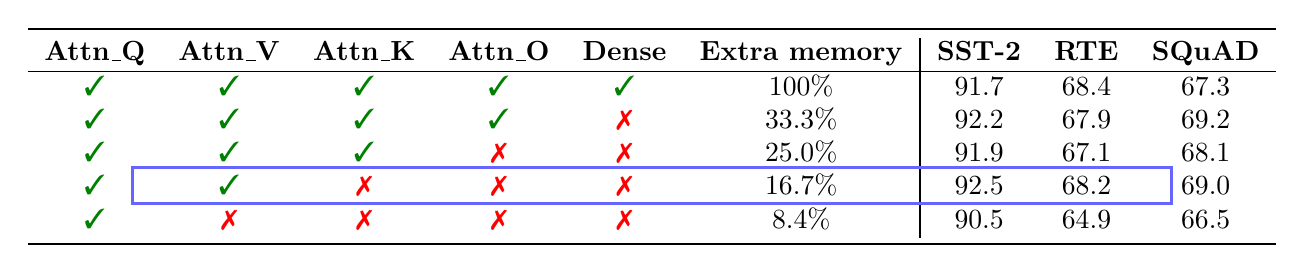
\begin{tikzpicture}
        \node (table) [inner sep=0pt] { % 嵌入表格
            \begin{tabular}{cccccc|ccc}
                \toprule
                \textbf{Attn\_Q} & \textbf{Attn\_V} & \textbf{Attn\_K} & \textbf{Attn\_O} & \textbf{Dense} & \textbf{Extra memory} & \textbf{SST-2} & \textbf{RTE} & \textbf{SQuAD} \\ \hline
                \cmark  & \cmark  & \cmark  & \cmark  & \cmark  & 100\%       & 91.7  & 68.4 & 67.3  \\
                \cmark  & \cmark  & \cmark  & \cmark  & \xmark  & 33.3\%      & 92.2  & 67.9 & 69.2  \\
                \cmark  & \cmark  & \cmark  & \xmark  & \xmark  & 25.0\%      & 91.9  & 67.1 & 68.1  \\
                \cmark  & \cmark  & \xmark  & \xmark  & \xmark  & 16.7\%      & 92.5  & 68.2 & 69.0  \\
                \cmark  & \xmark  & \xmark  & \xmark  & \xmark  & 8.4\%      & 90.5  & 64.9 & 66.5  \\
                \bottomrule
            \end{tabular}
        };

\draw[blue!60!white, very thick] (-6.6, -0.85) rectangle (6.6,-0.4);
    \end{tikzpicture}
    
    \label{ablation_layer}
\end{table*}

\subsection{Ablation for Strategies in ZO Projection Learning}
\label{ablation}


As discussed in Section~\ref{ZO}, we introduce two strategies, \emph{re-initialization} (Re-init) and \emph{projection clipping} (Clipping), to enhance projection learning and improve the stability of fine-tuning. The ablation results for these strategies, along with the corresponding loss curves, are shown in Figure~\ref{ablation_strategy}.

Overall (left in Figure~\ref{ablation_strategy}), omitting either Re-init or Clipping significantly diminishes the benefits of DiZO, with MeZO outperforming DiZO in these cases. Specifically, without Re-init, accuracy drops sharply, falling below MeZO. Similarly, without Clipping, while DiZO slightly outperforms MeZO on simpler datasets like SST-2, it suffers from severe model collapse on more challenging datasets, leading to a significant decline in accuracy.

From the loss curve trajectory (right in Figure~\ref{ablation_strategy}), without Re-init, DiZO loses its advantage in training acceleration, as the loss curve becomes noticeably slower to decrease. Without Clipping, the loss curve exhibits significant oscillations during certain training steps. This instability arises when projections are optimized to unsuitable values, such as extremely large or small magnitudes. These inappropriate projections cause substantial changes in model weights, leading to pronounced oscillations in the loss.

% \begin{table}
\begin{wraptable}{r}{8cm}
\centering
\vspace{-1em}
\caption{Ablation Study on Collaborative Strategy.}
\label{tab:ablation_stategy} 
\begin{tabular}{@{}lcccc@{}}
\toprule
                        & 2Wiki & PopQA & FQA  & M-RAG \\ \midrule
\modelname              & 65.2  & 44.8  & 72.8 & 50.0  \\ \midrule
\texttt{[No Retrieval]} & 41.6  & 24.3  & 58.2 & 42.2  \\
\texttt{[Retrieval]}    & 64.7  & 44.6  & 68.8 & 48.3  \\
\texttt{[Planning]}     & 65.5  & 46.9  & 74.8 & 50.4  \\ \bottomrule
\end{tabular}
\vspace{-0.5em}
% \end{table}
\end{wraptable}

% \begin{table}[t]
% % \setlength{\aboverulesep}{0pt}
% % \setlength{\belowrulesep}{0pt}
% % \setlength{\extrarowheight}{.75ex}  % 调整行高
% % \setlength{\tabcolsep}{2pt}
% \centering
% \caption{Ablation Study on Collaborative Strategy.}
% \label{tab:ablation_stategy} 
% \resizebox{0.99\linewidth}{!}{
% % \begin{small}
% \begin{tabular}{@{}lcccc@{}}
% \toprule
%                              & \textbf{FQA} & \textbf{M-RAG} & \textbf{FQA}   & \textbf{M-RAG}  \\
% LLM Servers                  & \multicolumn{2}{c}{Qwen2-72B} & \multicolumn{2}{c}{Llama3.3-70B} \\ \midrule
% \modelname                   & 72.8         & 50.0             & 71.6           & 47.2            \\ \midrule
% \texttt{[No Retrieval]} & 58.2         & 42.2           & 60.8           & 43.8            \\
% \texttt{[Retrieval]}    & 68.8         & 48.3           & 69.2           & 46.9            \\
% \texttt{[Planning]}     & 74.8         & 50.4           & 73.4           & 48.3            \\ \bottomrule
% \end{tabular}
% }
% % \end{small}
% \end{table}


\subsection{Does Other Alternative Strategies for Layer-wise Divergence Work?}
\label{alternative}

As discussed in Section~\ref{hypo}, our objective is to enhance layer-wise divergence in ZO optimization. Naturally, with consideration of this objective, one may raise two questions regarding the projection strategy we adopt: 1) Can we perform layer-wise projections on the learning rate? 2) When updating weight by projection at $t$-th iteration, why do we use the weights of pre-trained model $\bm{\theta}_0$ as the base of the update (shown in Eq.\ref{equ:4}) instead of the weights from the $(t-1)$-th iteration, $\bm{\theta}_{t-1}$?
% \begin{table}[h]
% \caption{Comparison on conducting projection on learning rate (LR) or use weight at $(t-1)$-th iteration $\bm{\theta}_{t-1}$ instead of the weight of the pre-trained model $\bm{\theta_{0}}$ as the base of projection.}
% \centering
% \begin{tabular}{lccccccccc}
% \toprule
% \multirow{2}{*}{\begin{tabular}[c]{@{}l@{}}Dataset\\ Task Type\end{tabular}} & \textbf{SST-2} & \textbf{RTE} & \textbf{CB} & \textbf{BoolQ} & \textbf{WSC} & \textbf{WIC} & \textbf{MultiRC} & \textbf{SQuAD}       & \textbf{DROP}       \\
%                                                                              & \multicolumn{7}{c}{--------------------------classification--------------------------}                        & \multicolumn{2}{c}{------generation------} \\ \hline
% LR projection                                                                & 56.3           & 54.2         & 50.0        & 47.6           & 36.5         & 52.7         & 44.4             & 29.8                 & 10.0                \\
% $\bm{\theta}_{t-1}$ projection                                                             & 94.2           & 81.2         & 82.1        & 72.2           & 63.8         & 65.8         & 71.6             & 78.4                 & 30.3                \\
% PeZO                                                                         & 94.6           & 80.8         & 82.7        & 77.7           & 59.8         & 64.0         & 72.8             & 77.9                 & 31.1   \\
% \bottomrule
% \end{tabular}
% \label{ablation_projection}
% \end{table}
\begin{table}[h]
\centering
\caption{Comparison on conducting projection on learning rate (LR) or use weight at $(t-1)$-th iteration $\bm{\theta}_{t-1}$ instead of the weight of the pre-trained model $\bm{\theta_{0}}$ as the base of projection. Results are obtained by fine-tuning OPT-2.7B.}
\vspace{5pt}
\begin{tabular}{lcccccc}
\toprule
\multirow{2}{*}{Dataset} & \multicolumn{2}{c}{\textbf{SST-2}}                         & \multicolumn{2}{c}{\textbf{RTE}}                           & \multicolumn{2}{c}{\textbf{SQuAD}}                         \\ \cline{2-7} 
                                                                             & Acc. & \begin{tabular}[c]{@{}c@{}}GPU\\ Hours\end{tabular} & Acc. & \begin{tabular}[c]{@{}c@{}}GPU\\ Hours\end{tabular} & F1.  & \begin{tabular}[c]{@{}c@{}}GPU\\ Hours\end{tabular} \\ \hline
MeZO                                                                         & 90.0 & 100.0\%                                                & 63.5 & 100.0\%                                                & 68.7 & 100.0\%                                                \\
LR projection                                                                & 89.5 & 94.7\%                                                & 63.9 & 108.5\%                                                & 67.9 & 89.8\%                                                \\
$\bm{\theta}_{t-1}$ projection                                                             & 90.7 & 87.8\%                                                & 64.5 & 90.3\%                                                & 67.2 & 88.4\%                                                \\
\rowcolor[gray]{.92}DiZO                                                                         & 92.5 & 55.7\%                                                & 68.2 & 62.3\%                                                & 69.0 & 65.4\%                                                \\ \bottomrule
\end{tabular}
\label{ablation_projection}
\end{table}

To answer the above two questions. We investigate two alternative projection strategies: 1) searching layer-wise ideal learning rate via ZO optimization and then applying the updates, and 2) conducting projection update based on $\bm{\theta}_{t-1}$ instead of $\bm{\theta}_{0}$. Results are illustrated in Table~\ref{ablation_projection}, neither approach achieves performance comparable to DiZO; both yield results closer to MeZO in terms of accuracy and required GPU hours.

% \begin{table*}[]
% \centering
% \scalebox{1}{
% \begin{tabular}{lccccccc}
% \toprule
% Task       & \textbf{\begin{tabular}[c]{@{}c@{}}Gradient\\ free\end{tabular}} & \textbf{\begin{tabular}[c]{@{}c@{}}Parameter\\ efficient\end{tabular}} & \textbf{\begin{tabular}[c]{@{}c@{}}Peak \\ memory\end{tabular}} & \textbf{\begin{tabular}[c]{@{}c@{}}Averaged\\ memory\end{tabular}} & \textbf{Throughput} & \textbf{Iterations} & \textbf{\begin{tabular}[c]{@{}c@{}}GPU \\ hours\end{tabular}} \\ \hline
% MeZO       & \cmark                                            & \xmark                                                  & 13.6 GB                                                      & 13.6 GB                                                        & 3.28 it/s          & 100.0\%                                                            & 100.0\%                                                    \\
% HiZOO      & \cmark                                            & \xmark                                                  & 23.7 GB                                                      & 23.7 GB                                                        & 2.22 it/s          & 59.2\%                                                            & 87.4\%                                                    \\
% \rowcolor[gray]{.92}DiZO       & \cmark                                            & \xmark                                                  & 15.1 GB                                                    & 15.1 GB                                                        & 2.85 it/s          & 51.8\%                                                            & 59.7\%                                                    \\ \hline
% MeZO LoRA  & \cmark                                            & \cmark                                                  & 12.9 GB                                                     & 12.9 GB                                                        & 5.56 it/s          & 74.1\%                                                            & 85.7\%                                                    \\
% HiZOO LoRA & \cmark                                            & \cmark                                                  & 22.9 GB                                                      & 22.9 GB                                                        & 3.70 it/s          & 46.3\%                                                            & 82.0\%                                                    \\
% \rowcolor[gray]{.92}DiZO LoRA  & \cmark                                            & \cmark                                                  & 14.4 GB                                                      & 14.4 GB                                                        & 4.42 it/s          & 38.9\%                                                            & 57.6\%    \\ \hline
% FT         & \xmark                                            & \xmark                                                  & 45.4 GB                                                     & 45.4 GB                                                        & 1.81 it/s          & 9.3\%                                                            & 16.8\%                                                    \\
% LoRA       & \xmark                                            & \xmark                                                  & 18.4 GB                                                     & 18.4 GB                                                        & 4.50 it/s          & 5.6\%                                                            & 4.3\%                                                    \\
% DiZO\textsuperscript{\textdagger}       & \neutral                                          & \xmark                                                  & 17.8  GB                                                     & 15.7 GB                                                        & 2.63 it/s          & 33.3\%                                                            & 41.5\%                                                    \\
% DiZO LoRA\textsuperscript{\textdagger}  & \neutral                                          & \cmark                                                  & 16.1 GB                                                     & 14.7 GB                                                        & 4.16 it/s          & 22.2\%                                                            & 17.5\%                                                    \\
% \bottomrule
% \end{tabular}
% }
% \caption{Memory utilization and speed test on OPT-2.7B on SST-2 dataset (35 tokens per example on average). \neutral: partial gradient-free; \cmark: gradient-free; \xmark: gradient-based. DiZO\textsuperscript{\textdagger}: searching projection with Adam.}
% \label{memory_speed_sst2}
% \end{table*}

\begin{table*}[]
\centering
\caption{Memory utilization and speed test on OPT-2.7B on SST-2 dataset (35 tokens per example on average). \neutral: partial gradient-free; \cmark: gradient-free; \xmark: gradient-based. DiZO\textsuperscript{\textdagger}: searching projection with Adam.}
\vspace{5pt}
\scalebox{1}{
\begin{tabular}{lccccccc}
\toprule
Task Type       & \textbf{\begin{tabular}[c]{@{}c@{}}Gradient\\ Free\end{tabular}} & \textbf{\begin{tabular}[c]{@{}c@{}}LoRA\\ Added\end{tabular}} & \textbf{\begin{tabular}[c]{@{}c@{}}Peak \\ Memory\end{tabular}} & \textbf{\begin{tabular}[c]{@{}c@{}}Averaged\\ Memory\end{tabular}} & \textbf{Throughput} & \textbf{\begin{tabular}[c]{@{}c@{}}\#Train \\ Iter.\end{tabular}} & \textbf{\begin{tabular}[c]{@{}c@{}}GPU \\ Hours\end{tabular}} \\ \hline
FT         & \xmark                                            & \xmark                                                  & 45.4 GB                                                     & 45.4 GB                                                        & 1.81 it/s          & 9.3\%                                                            & 16.8\%                                                    \\
LoRA       & \xmark                                            & \cmark                                                  & 18.4 GB                                                     & 18.4 GB                                                        & 4.50 it/s          & 5.6\%                                                            & 4.3\%                                                    \\
DiZO\textsuperscript{\textdagger}       & \neutral                                          & \xmark                                                  & 17.8  GB                                                     & 15.7 GB                                                        & 2.63 it/s          & 33.3\%                                                            & 41.5\%                                                    \\
DiZO LoRA\textsuperscript{\textdagger}  & \neutral                                          & \cmark                                                  & 16.1 GB                                                     & 14.7 GB                                                        & 4.16 it/s          & 22.2\%                                                            & 17.5\%                                                    \\ \hline
MeZO       & \cmark                                            & \xmark                                                  & 6.8 GB                                                      & 6.8 GB                                                        & 3.28 it/s          & 100.0\%                                                            & 100.0\%                                                    \\
HiZOO      & \cmark                                            & \xmark                                                  & 11.8 GB                                                      & 11.8 GB                                                        & 2.22 it/s          & 59.2\%                                                            & 87.4\%                                                    \\
\rowcolor[gray]{.92}DiZO       & \cmark                                            & \xmark                                                  & 7.5 GB                                                    & 7.5 GB                                                        & 3.05 it/s          & 51.8\%                                                            & 55.7\%                                                    \\ \hline
MeZO LoRA  & \cmark                                            & \cmark                                                  & 6.5 GB                                                     & 6.5 GB                                                        & 5.56 it/s          & 74.1\%                                                            & 43.7\%                                                    \\
HiZOO LoRA & \cmark                                            & \cmark                                                  & 11.5 GB                                                      & 11.5 GB                                                        & 3.70 it/s          & 46.3\%                                                            & 41.0\%                                                    \\
\rowcolor[gray]{.92}DiZO LoRA  & \cmark                                            & \cmark                                                  & 7.2 GB                                                      & 7.2 GB                                                        & 4.92 it/s          & 38.9\%                                                            & 25.9\%    \\ 
\bottomrule
\end{tabular}
}

\label{memory_speed_sst2}
\end{table*}
\begin{table*}[]
\centering
\caption{Memory utilization and speed test on OPT-2.7B on SQuAD dataset (300 tokens per example on average). \neutral: partial gradient-free; \cmark: gradient-free; \xmark: gradient-based. DiZO\textsuperscript{\textdagger}: searching projection with Adam.}
\vspace{5pt}
\scalebox{1}{
\begin{tabular}{lccccccc}
\toprule
Task Type       & \textbf{\begin{tabular}[c]{@{}c@{}}Gradient\\ Free\end{tabular}} & \textbf{\begin{tabular}[c]{@{}c@{}}LoRA\\ Added\end{tabular}} & \textbf{\begin{tabular}[c]{@{}c@{}}Peak \\ Memory\end{tabular}} & \textbf{\begin{tabular}[c]{@{}c@{}}Averaged\\ Memory\end{tabular}} & \textbf{Throughput} & \textbf{\begin{tabular}[c]{@{}c@{}}\#Train \\ Iter.\end{tabular}} & \textbf{\begin{tabular}[c]{@{}c@{}}GPU \\ Hours\end{tabular}} \\ \hline
FT         & \xmark                                            & \xmark                                                  & 73.5 GB                                                      & 73.5 GB                                                        & 0.36 it/s          & 7.5\%                                                            & 27.7\%                                                   \\
LoRA       & \xmark                                            & \cmark                                                  & 58.5 GB                                                      & 58.5 GB                                                       & 0.73 it/s          & 6.3\%                                                            & 11.5\%                                                    \\
DiZO\textsuperscript{\textdagger}       & \neutral                                          & \xmark                                                  & 57.8 GB                                                      & 20.3 GB                                                        & 1.22 it/s          & 41.7\%                                                            & 45.5\%                                                    \\
DiZO LoRA\textsuperscript{\textdagger}  & \neutral                                          & \cmark                                                  & 49.4 GB                                                      & 19.9 GB                                                        & 2.44 it/s          & 31.7\%                                                            & 17.3\%                                                    \\  \hline
MeZO       & \cmark                                            & \xmark                                                  & 8.4 GB                                                      & 8.4 GB                                                        & 1.33 it/s          & 100.0\%                                                            & 100.0\%                                                    \\
HiZOO      & \cmark                                            & \xmark                                                  & 12.3 GB                                                      & 13.3 GB                                                        & 0.97 it/s          & 66.7\%                                                            & 91.5\%                                                  \\
\rowcolor[gray]{.92}DiZO       & \cmark                                            & \xmark                                                  & 9.7 GB                                                      & 9.7 GB                                                        & 1.22 it/s          & 60.0\%                                                            & 65.4\%                                                    \\ \hline
MeZO LoRA  & \cmark                                            & \cmark                                                  & 8.4 GB                                                      & 8.4 GB                                                        & 2.80 it/s          & 73.3\%                                                            & 34.8\%                                                    \\
HiZOO LoRA & \cmark                                            & \cmark                                                  & 11.6 GB                                                      & 12.6 GB                                                        & 2.10 it/s          & 56.7\%                                                            & 35.9\%                                                    \\
\rowcolor[gray]{.92}DiZO LoRA  & \cmark                                            & \cmark                                                  & 9.6 GB                                                      & 9.6 GB                                                        & 2.49 it/s          & 45.0\%                                                            & 24.0\%    \\
\bottomrule
\end{tabular}
}

\label{memory_squad}
\end{table*}

We attribute this phenomenon to the high noise inherent in each ZO update, which relies on random perturbations and thus produces a highly imprecise update direction. In contrast, DiZO projects the optimization direction between the pre-trained and fine-tuned models, and this direction is supposed to be correct. Otherwise, the entire optimization would fail and the loss would not decrease.  Moreover, recent studies suggest that the fine-tuned model is often less robust than their pre-trained version due to catastrophic forgetting~\cite{dong2021should, oh2023towards, zhai2023investigating, wang2024pre}. Maintaining a connection with the pre-trained model helps robustify the fine-tuning process and mitigate some of the noise introduced by ZO’s random perturbations.




% ~\\
% \newpage


% \subsection{PyTorch-style code for gradient-free searching of projections}
% \label{code}




\section{More Experiment Results}

\subsection{Memory and Speed Analysis}
\label{speed}
We present the memory and speed results for OPT-2.7B on the SST-2 and SQuAD datasets in Table~\ref{memory_speed_sst2} and Table~\ref{memory_squad}, respectively. DiZO significantly reduces the number of required iterations while maintaining throughput comparable to MeZO, leading to substantially fewer training GPU hours. In contrast, HiZOO achieves only modest iteration savings and further reduces the throughput of MeZO by approximately 1.5× due to its reliance on second-order information estimation. As a result, HiZOO offers only a slight improvement over MeZO in terms of training GPU hours. In some cases, such as HiZOO combined with LoRA on SQuAD, it even consumes more training GPU hours than MeZO with LoRA.





\subsection{Llama Experiments}
\label{Llama}

To demonstrate the broader applicability of DiZO, we conducted experiments on the Llama-series models. The results for Llama3-3B and Llama3-8B are presented in Table~\ref{Llama-3B} and Table~\ref{Llama-8B}, respectively. DiZO consistently outperforms MeZO across both the 3B and 8B Llama models.

However, we observed that ZO LoRA performs poorly with Llama models (including DiZO, MeZO and HiZOO). The loss value remains stagnant, and the resulting accuracy is comparable to or even worse than zero-shot results. We leave it to future work to investigate why ZO LoRA fails with Llama models. We suspect that this limitation may be related to the Group Query Attention (GQA)~\cite{ainslie2023gqa} mechanism employed in Llama3.
\begin{table*}[t!] \resizebox{\textwidth}{!}{\begin{tabular}{l||cc|cc|cc|cc|cc|c|c|c|c|c|c|c}
\toprule
\multirow{2}{*}{\textbf{UQ Method}} & \multicolumn{2}{c|}{\textbf{XSUM}} & \multicolumn{2}{c|}{\textbf{SamSum}} & \multicolumn{2}{c|}{\textbf{CNN}}& \multicolumn{2}{c|}{\textbf{PubMedQA}} & \multicolumn{2}{c|}{\textbf{MedQUAD}} & \multicolumn{1}{c|}{\textbf{TruthfulQA}}& \multicolumn{1}{c|}{\textbf{CoQA}} & \multicolumn{1}{c|}{\textbf{SciQ}} & \multicolumn{1}{c|}{\textbf{TriviaQA}} & \multicolumn{1}{c|}{\textbf{GSM8k}} & \multicolumn{1}{c|}{\textbf{MMLU}} & \multirow{2}{*}{\textbf{Mean Rank}} \\ \cline{2-17}
    & \textbf{ROUGE-L} & \textbf{AlignScore} & \textbf{ROUGE-L} & \textbf{AlignScore} & \textbf{ROUGE-L} & \textbf{AlignScore} & \textbf{ROUGE-L} & \textbf{AlignScore} & \textbf{ROUGE-L} & \textbf{AlignScore} & \textbf{AlignScore} & \textbf{AlignScore} & \textbf{AlignScore}& \textbf{AlignScore} & \textbf{Accuracy}& \textbf{Accuracy}& \\
\midrule
Maximum Sequence Probability & \large\cellcolor[rgb]{0.6449978024117646,0.6934178380941176,0.9144631795921568} -.343 & \large\cellcolor[rgb]{0.61490285,0.649358983,0.8768415764999999} -.128 & \large\cellcolor[rgb]{0.9053078374137256,0.6343985308588236,0.6177138057666667} \underline{.452} & \large\cellcolor[rgb]{0.9613407263117647,0.9142840690588235,0.8885271948941176} .218 & \large\cellcolor[rgb]{0.6741616707058824,0.7328555732549019,0.9441730814705882} .021 & \large\cellcolor[rgb]{0.866948893627451,0.9100089393823529,0.9853621830490196} .096 & \large\cellcolor[rgb]{0.61490285,0.649358983,0.8768415764999999} -.155 & \large\cellcolor[rgb]{0.6944259359764706,0.7581492177882353,0.9606867415411764} -.011 & \large\cellcolor[rgb]{0.9797588292352941,0.8834864272549019,0.8370723575196078} .297 & \large\cellcolor[rgb]{0.9772829111803922,0.8895272809333333,0.8462654299039216} .356 & \large\cellcolor[rgb]{0.9720272867117647,0.7765767393745098,0.7177742451568627} .277 & \large\cellcolor[rgb]{0.8925766523392157,0.6104255443607843,0.6058364385039215} .450 & \large\cellcolor[rgb]{0.947942297417647,0.7165372783529411,0.6693403172588235} \underline{.582} & \large\cellcolor[rgb]{0.8790560841823529,0.5840607685176471,0.5944135352882353} .687 & \large\cellcolor[rgb]{0.9613407263117647,0.9142840690588235,0.8885271948941176} .380 & \large\cellcolor[rgb]{0.8362689763627451,0.8914307235588235,0.9959909503117648} .405 & \large\cellcolor[rgb]{0.8816813900509803,0.917546110909804,0.9778288382784314} 7.81 \\
Perplexity & \large\cellcolor[rgb]{0.61490285,0.649358983,0.8768415764999999} -.384 & \large\cellcolor[rgb]{0.6520871435019608,0.7034724414196079,0.9226313633490196} -.108 & \large\cellcolor[rgb]{0.6766845796941177,0.736034329145098,0.9462852021294117} .080 & \large\cellcolor[rgb]{0.9747269947588235,0.7861939559392157,0.7267214884509805} .308 & \large\cellcolor[rgb]{0.852836579,0.50777808,0.575116406} \textbf{.150} & \large\cellcolor[rgb]{0.852836579,0.50777808,0.575116406} \textbf{.242} & \large\cellcolor[rgb]{0.9842498738333334,0.8369886898862745,0.7783246280235294} .215 & \large\cellcolor[rgb]{0.61490285,0.649358983,0.8768415764999999} -.044 & \large\cellcolor[rgb]{0.9150932609745098,0.6523663817764705,0.6274457140333334} \underline{.425} & \large\cellcolor[rgb]{0.9765268001235294,0.7926054336490196,0.7326863173137255} .438 & \large\cellcolor[rgb]{0.9296925499352942,0.9322154837294118,0.9360552653941177} .178 & \large\cellcolor[rgb]{0.8925766523392157,0.6104255443607843,0.6058364385039215} .450 & \large\cellcolor[rgb]{0.61490285,0.649358983,0.8768415764999999} .197 & \large\cellcolor[rgb]{0.8763519705509804,0.5787878133490196,0.5921289546450981} .689 & \large\cellcolor[rgb]{0.8466606424117646,0.8981570658529412,0.9931538902647059} .259 & \large\cellcolor[rgb]{0.7285232392627451,0.797002774964706,0.9815146148450979} .308 & \large\cellcolor[rgb]{0.9133921582352942,0.9291026777686274,0.9534763223137255} 7.38 \\\midrule
DegMat NLI Score Entail. & \large\cellcolor[rgb]{0.9398111318019609,0.9290874692039215,0.9229219340686274} .017 & \large\cellcolor[rgb]{0.9842498738333334,0.8369886898862745,0.7783246280235294} .093 & \large\cellcolor[rgb]{0.9216790870960784,0.9309098270078431,0.945008558445098} .250 & \large\cellcolor[rgb]{0.9678868848333333,0.9061183506196079,0.873578236792157} .226 & \large\cellcolor[rgb]{0.9514243351588236,0.9223978252941176,0.9059849168705882} .084 & \large\cellcolor[rgb]{0.9704394715,0.9027982014117647,0.8675832782352941} .144 & \large\cellcolor[rgb]{0.8863529743019607,0.9194891086196078,0.9746593799568628} .064 & \large\cellcolor[rgb]{0.876805309,0.9151164254999999,0.9804355785000001} .058 & \large\cellcolor[rgb]{0.6817303976705882,0.7423918409254902,0.9505094434470589} .066 & \large\cellcolor[rgb]{0.7907430740941177,0.8567252977647059,0.9991571764705882} .162 & \large\cellcolor[rgb]{0.8933603506784313,0.9224036051843137,0.9699051924745098} .156 & \large\cellcolor[rgb]{0.9385746672999999,0.6973227293333333,0.6558619128666667} .420 & \large\cellcolor[rgb]{0.9547297988764706,0.919693239882353,0.9001656762117647} .446 & \large\cellcolor[rgb]{0.852836579,0.50777808,0.575116406} \textbf{.714} & \large\cellcolor[rgb]{0.9438760079745099,0.9270202487490196,0.9173357361078431} .357 & \large\cellcolor[rgb]{0.6402749751176471,0.6867115845411764,0.909005371654902} .224 & \large\cellcolor[rgb]{0.9256858185156862,0.9315626553686274,0.9405319119196078} 7.19 \\
Eccentricity NLI Score Entail. & \large\cellcolor[rgb]{0.9046643351764705,0.9264869997764706,0.9611612942352941} -.036 & \large\cellcolor[rgb]{0.9046643351764705,0.9264869997764706,0.9611612942352941} .013 & \large\cellcolor[rgb]{0.7961779297490197,0.861396014627451,0.9997169374117647} .160 & \large\cellcolor[rgb]{0.8283414337745099,0.8859032383823529,0.9974569188764706} .117 & \large\cellcolor[rgb]{0.7048055483372548,0.7703792543686274,0.9677723612431373} .028 & \large\cellcolor[rgb]{0.7365350864941176,0.8055387188078431,0.9853167941313725} .050 & \large\cellcolor[rgb]{0.8492270432274509,0.8997249420568627,0.9922887283509805} .033 & \large\cellcolor[rgb]{0.7798733627843137,0.8473838640392157,0.9980376545882352} .021 & \large\cellcolor[rgb]{0.6892991246352941,0.7519281085960785,0.9568458054235294} .070 & \large\cellcolor[rgb]{0.6691882557215687,0.7264093044156863,0.9396585384392157} .060 & \large\cellcolor[rgb]{0.8309839479705883,0.8877457334411765,0.9969682626882352} .122 & \large\cellcolor[rgb]{0.9513294646843138,0.7239693735803922,0.6748606867705882} .409 & \large\cellcolor[rgb]{0.953077067017647,0.9210455325882353,0.9030752965411765} .444 & \large\cellcolor[rgb]{0.9077541933039216,0.6388904935882354,0.6201467828333334} .654 & \large\cellcolor[rgb]{0.9727701494549019,0.8993028702666667,0.8615527086490196} .403 & \large\cellcolor[rgb]{0.7311771982901961,0.7999150558117647,0.9829285958960784} .312 & \large\cellcolor[rgb]{0.7022106452470588,0.7673217452235295,0.966000956317647} 10.00 \\
EigValLaplacian NLI Score Entail. & \large\cellcolor[rgb]{0.9398111318019609,0.9290874692039215,0.9229219340686274} .016 & \large\cellcolor[rgb]{0.9830083599196078,0.8230648707941176,0.7629451741294118} .099 & \large\cellcolor[rgb]{0.9216790870960784,0.9309098270078431,0.945008558445098} .251 & \large\cellcolor[rgb]{0.9653342981666666,0.909438499827451,0.8795731953490196} .224 & \large\cellcolor[rgb]{0.9613407263117647,0.9142840690588235,0.8885271948941176} .087 & \large\cellcolor[rgb]{0.9691631781666666,0.9044582760156863,0.8705807575137254} .143 & \large\cellcolor[rgb]{0.8743412051568626,0.9138395539705882,0.9816672296372548} .054 & \large\cellcolor[rgb]{0.866948893627451,0.9100089393823529,0.9853621830490196} .054 & \large\cellcolor[rgb]{0.6691882557215687,0.7264093044156863,0.9396585384392157} .056 & \large\cellcolor[rgb]{0.7880256462666666,0.8543899393333334,0.9988772960000001} .160 & \large\cellcolor[rgb]{0.8863529743019607,0.9194891086196078,0.9746593799568628} .152 & \large\cellcolor[rgb]{0.9028614815235294,0.6299065681294118,0.6152808287} .444 & \large\cellcolor[rgb]{0.9003004236470589,0.9251791607803921,0.9650037801960785} .398 & \large\cellcolor[rgb]{0.8952807659705883,0.6156984995294118,0.6081210191470588} .669 & \large\cellcolor[rgb]{0.9236824528058823,0.9312362411882353,0.942770235182353} .335 & \large\cellcolor[rgb]{0.7690021078509803,0.8374507968235294,0.9958609467764705} .344 & \large\cellcolor[rgb]{0.8910245585529412,0.9214321063294117,0.9714899216352941} 7.69 \\
Lexical Similarity ROUGE-L & \large\cellcolor[rgb]{0.9691631781666666,0.9044582760156863,0.8705807575137254} .071 & \large\cellcolor[rgb]{0.9772829111803922,0.8895272809333333,0.8462654299039216} .066 & \large\cellcolor[rgb]{0.9802905992117648,0.8812505092627452,0.8339817735509804} .320 & \large\cellcolor[rgb]{0.953077067017647,0.9210455325882353,0.9030752965411765} .209 & \large\cellcolor[rgb]{0.9622044108411765,0.7492947789176471,0.6945295061352941} .123 & \large\cellcolor[rgb]{0.9296925499352942,0.9322154837294118,0.9360552653941177} .122 & \large\cellcolor[rgb]{0.9640580048333334,0.9110985744313725,0.882570674627451} .144 & \large\cellcolor[rgb]{0.8336264621666667,0.8895882285,0.9964796065} .041 & \large\cellcolor[rgb]{0.9459084460607843,0.9259866385215686,0.914542637127451} .252 & \large\cellcolor[rgb]{0.7554121621254901,0.8246983074117646,0.9925393881882354} .132 & \large\cellcolor[rgb]{0.61490285,0.649358983,0.8768415764999999} .008 & \large\cellcolor[rgb]{0.9575785619705882,0.7384632635882353,0.686089707382353} .403 & \large\cellcolor[rgb]{0.8492270432274509,0.8997249420568627,0.9922887283509805} .360 & \large\cellcolor[rgb]{0.9326956664686274,0.6855638360235294,0.6478844782078431} .621 & \large\cellcolor[rgb]{0.9840526685,0.8342375980588236,0.7752431104705884} .467 & \large\cellcolor[rgb]{0.7311771982901961,0.7999150558117647,0.9829285958960784} .311 & \large\cellcolor[rgb]{0.8816813900509803,0.917546110909804,0.9778288382784314} 7.81 \\
SAR & \large\cellcolor[rgb]{0.9547297988764706,0.919693239882353,0.9001656762117647} .040 & \large\cellcolor[rgb]{0.9547297988764706,0.919693239882353,0.9001656762117647} .044 & \large\cellcolor[rgb]{0.9704394715,0.9027982014117647,0.8675832782352941} .300 & \large\cellcolor[rgb]{0.9596879944529412,0.9156363617647059,0.8914368152235295} .217 & \large\cellcolor[rgb]{0.9683898066058824,0.766374750054902,0.7090466697431372} .120 & \large\cellcolor[rgb]{0.9802905992117648,0.8812505092627452,0.8339817735509804} .154 & \large\cellcolor[rgb]{0.9459084460607843,0.9259866385215686,0.914542637127451} .122 & \large\cellcolor[rgb]{0.8096589725941177,0.8720603673823529,0.9994654594098039} .032 & \large\cellcolor[rgb]{0.9736727018,0.8973477524,0.8584952529000001} .286 & \large\cellcolor[rgb]{0.8283414337745099,0.8859032383823529,0.9974569188764706} .192 & \large\cellcolor[rgb]{0.7961779297490197,0.861396014627451,0.9997169374117647} .105 & \large\cellcolor[rgb]{0.864597965917647,0.5433394684235294,0.5836202017019608} \underline{.465} & \large\cellcolor[rgb]{0.9497716033000001,0.923750118,0.9088945372} .440 & \large\cellcolor[rgb]{0.8557769257294118,0.5166684271058823,0.5772423549254901} \underline{.710} & \large\cellcolor[rgb]{0.9849255762058824,0.8479150297647058,0.7906558870392157} .455 & \large\cellcolor[rgb]{0.7022106452470588,0.7673217452235295,0.966000956317647} .284 & \large\cellcolor[rgb]{0.9640580048333334,0.9110985744313725,0.882570674627451} 6.50 \\
Semantic Entropy & \large\cellcolor[rgb]{0.9547297988764706,0.919693239882353,0.9001656762117647} .041 & \large\cellcolor[rgb]{0.9024823794117647,0.9258330802784314,0.9630825372156863} .012 & \large\cellcolor[rgb]{0.9763803588352942,0.8914823988,0.8493228856529411} .311 & \large\cellcolor[rgb]{0.9497716033000001,0.923750118,0.9088945372} .206 & \large\cellcolor[rgb]{0.9276891842254902,0.9318890695490196,0.9382935886568627} .077 & \large\cellcolor[rgb]{0.866948893627451,0.9100089393823529,0.9853621830490196} .096 & \large\cellcolor[rgb]{0.8863529743019607,0.9194891086196078,0.9746593799568628} .064 & \large\cellcolor[rgb]{0.815044265017647,0.8762581198529411,0.9992540061705882} .034 & \large\cellcolor[rgb]{0.6970208390666667,0.7612067269333334,0.9624581464666666} .075 & \large\cellcolor[rgb]{0.61490285,0.649358983,0.8768415764999999} .007 & \large\cellcolor[rgb]{0.9176723556764705,0.9302569986470588,0.9494852049705882} .171 & \large\cellcolor[rgb]{0.9423217193470588,0.7050085489411765,0.6612532746235295} .416 & \large\cellcolor[rgb]{0.9717157648333333,0.9011381268078431,0.8645857989568628} .466 & \large\cellcolor[rgb]{0.8952807659705883,0.6156984995294118,0.6081210191470588} .669 & \large\cellcolor[rgb]{0.9808223691882353,0.8790145912705882,0.830891189582353} .424 & \large\cellcolor[rgb]{0.6355521478235294,0.6800053309882352,0.9035475637176471} .220 & \large\cellcolor[rgb]{0.8389114905588235,0.8932732186176471,0.9955022941235294} 8.38 \\
SentenceSAR & \large\cellcolor[rgb]{0.866948893627451,0.9100089393823529,0.9853621830490196} -.085 & \large\cellcolor[rgb]{0.815044265017647,0.8762581198529411,0.9992540061705882} -.032 & \large\cellcolor[rgb]{0.9377786937156862,0.9301210794313726,0.9257150330490196} .264 & \large\cellcolor[rgb]{0.9580352625941176,0.9169886544705883,0.8943464355529411} .215 & \large\cellcolor[rgb]{0.8336264621666667,0.8895882285,0.9964796065} .055 & \large\cellcolor[rgb]{0.8543598448588235,0.9028606944647058,0.9905584045235294} .091 & \large\cellcolor[rgb]{0.806966326382353,0.8699614911470588,0.9995711860294118} -.000 & \large\cellcolor[rgb]{0.7392311256470588,0.8082818218039216,0.9863604477156862} .006 & \large\cellcolor[rgb]{0.61490285,0.649358983,0.8768415764999999} .015 & \large\cellcolor[rgb]{0.6402749751176471,0.6867115845411764,0.909005371654902} .033 & \large\cellcolor[rgb]{0.9398111318019609,0.9290874692039215,0.9229219340686274} .185 & \large\cellcolor[rgb]{0.852836579,0.50777808,0.575116406} \textbf{.472} & \large\cellcolor[rgb]{0.9765268001235294,0.7926054336490196,0.7326863173137255} .543 & \large\cellcolor[rgb]{0.8616576191882352,0.5344491213176471,0.5814942527764706} .703 & \large\cellcolor[rgb]{0.7232153212078432,0.7911782132705882,0.9786866527431373} .151 & \large\cellcolor[rgb]{0.7662841187058823,0.8349002989411765,0.9951966350588235} .343 & \large\cellcolor[rgb]{0.806966326382353,0.8699614911470588,0.9995711860294118} 8.75 \\\midrule
Factoscope & \large\cellcolor[rgb]{0.9497716033000001,0.923750118,0.9088945372} .032 & \large\cellcolor[rgb]{0.8204138911862745,0.8803757532058823,0.9989228874411764} -.029 & \large\cellcolor[rgb]{0.61490285,0.649358983,0.8768415764999999} .034 & \large\cellcolor[rgb]{0.61490285,0.649358983,0.8768415764999999} -.024 & \large\cellcolor[rgb]{0.61490285,0.649358983,0.8768415764999999} .007 & \large\cellcolor[rgb]{0.61490285,0.649358983,0.8768415764999999} .004 & \large\cellcolor[rgb]{0.7608481404156863,0.8297993031764705,0.9938680116235294} -.035 & \large\cellcolor[rgb]{0.7258692802352941,0.794090494117647,0.9801006337941176} .001 & \large\cellcolor[rgb]{0.9765268001235294,0.7926054336490196,0.7326863173137255} .358 & \large\cellcolor[rgb]{0.9802450306647059,0.8081382119705882,0.7477333002470589} .428 & \large\cellcolor[rgb]{0.6286169883529411,0.6698302759882353,0.8948307002647058} .017 & \large\cellcolor[rgb]{0.8840171821764706,0.9185176097647059,0.976244109117647} .242 & \large\cellcolor[rgb]{0.7825907906117646,0.8497192224705882,0.9983175350588236} .316 & \large\cellcolor[rgb]{0.61490285,0.649358983,0.8768415764999999} -.046 & \large\cellcolor[rgb]{0.61490285,0.649358983,0.8768415764999999} .048 & \large\cellcolor[rgb]{0.9423217193470588,0.7050085489411765,0.6612532746235295} \underline{.727} & \large\cellcolor[rgb]{0.61490285,0.649358983,0.8768415764999999} 11.19 \\
EigenScore & \large\cellcolor[rgb]{0.9547297988764706,0.919693239882353,0.9001656762117647} .041 & \large\cellcolor[rgb]{0.931695915645098,0.9325418979098039,0.9338169421313726} .029 & \large\cellcolor[rgb]{0.8492270432274509,0.8997249420568627,0.9922887283509805} .196 & \large\cellcolor[rgb]{0.8792694128431373,0.9163932970294117,0.9792039273627451} .150 & \large\cellcolor[rgb]{0.7635661295607843,0.8323498010588235,0.9945323233411765} .040 & \large\cellcolor[rgb]{0.7232153212078432,0.7911782132705882,0.9786866527431373} .045 & \large\cellcolor[rgb]{0.8980319349294118,0.9243466028941176,0.9667357341529412} .074 & \large\cellcolor[rgb]{0.7961779297490197,0.861396014627451,0.9997169374117647} .027 & \large\cellcolor[rgb]{0.6594161915960784,0.7133025255607843,0.9299287241019608} .050 & \large\cellcolor[rgb]{0.6520871435019608,0.7034724414196079,0.9226313633490196} .043 & \large\cellcolor[rgb]{0.6402749751176471,0.6867115845411764,0.909005371654902} .023 & \large\cellcolor[rgb]{0.9575785619705882,0.7384632635882353,0.686089707382353} .402 & \large\cellcolor[rgb]{0.866948893627451,0.9100089393823529,0.9853621830490196} .373 & \large\cellcolor[rgb]{0.9326956664686274,0.6855638360235294,0.6478844782078431} .619 & \large\cellcolor[rgb]{0.9818859091411765,0.8745427552862746,0.8247100216450981} .430 & \large\cellcolor[rgb]{0.61490285,0.649358983,0.8768415764999999} .196 & \large\cellcolor[rgb]{0.6691882557215687,0.7264093044156863,0.9396585384392157} 10.44 \\
SAPLMA & \large\cellcolor[rgb]{0.9845960255235294,0.8529178378588236,0.7968521304901961} .144 & \large\cellcolor[rgb]{0.9607031106137255,0.7457102085921569,0.6917042176882353} .129 & \large\cellcolor[rgb]{0.9133921582352942,0.9291026777686274,0.9534763223137255} .243 & \large\cellcolor[rgb]{0.9720272867117647,0.7765767393745098,0.7177742451568627} \underline{.313} & \large\cellcolor[rgb]{0.9528917390058824,0.727592846082353,0.6776679419235294} .126 & \large\cellcolor[rgb]{0.9807976965156863,0.8111235437352942,0.7507756750235295} \underline{.179} & \large\cellcolor[rgb]{0.9791396989627451,0.8021675484411765,0.7416485506941177} .240 & \large\cellcolor[rgb]{0.9720272867117647,0.7765767393745098,0.7177742451568627} .155 & \large\cellcolor[rgb]{0.9367011412764705,0.6934798195294117,0.6531662319882353} .407 & \large\cellcolor[rgb]{0.9460687713941176,0.7126943685490196,0.6666446363803922} .490 & \large\cellcolor[rgb]{0.8123516188058824,0.8741592436176471,0.9993597327901961} .112 & \large\cellcolor[rgb]{0.61490285,0.649358983,0.8768415764999999} .082 & \large\cellcolor[rgb]{0.888688766427451,0.9204606074745099,0.9730746507960784} .388 & \large\cellcolor[rgb]{0.9791396989627451,0.8021675484411765,0.7416485506941177} .522 & \large\cellcolor[rgb]{0.9028614815235294,0.6299065681294118,0.6152808287} \underline{.598} & \large\cellcolor[rgb]{0.9112102024705883,0.9284487582705883,0.9553975652941177} .481 & \large\cellcolor[rgb]{0.9848414898333333,0.8452419653686274,0.7875691806823529} 5.50 \\\midrule\midrule
HUQ-SATRMD & \large\cellcolor[rgb]{0.852836579,0.50777808,0.575116406} \textbf{.395} & \large\cellcolor[rgb]{0.852836579,0.50777808,0.575116406} \textbf{.187} & \large\cellcolor[rgb]{0.852836579,0.50777808,0.575116406} \textbf{.486} & \large\cellcolor[rgb]{0.9796923648137255,0.8051528802058824,0.7446909254705882} .297 & \large\cellcolor[rgb]{0.9528917390058824,0.727592846082353,0.6776679419235294} .126 & \large\cellcolor[rgb]{0.7311771982901961,0.7999150558117647,0.9829285958960784} .048 & \large\cellcolor[rgb]{0.8817601978137255,0.5893337236862746,0.5966981159313726} \underline{.351} & \large\cellcolor[rgb]{0.852836579,0.50777808,0.575116406} \textbf{.211} & \large\cellcolor[rgb]{0.9575785619705882,0.7384632635882353,0.686089707382353} .386 & \large\cellcolor[rgb]{0.9326956664686274,0.6855638360235294,0.6478844782078431} \underline{.506} & \large\cellcolor[rgb]{0.9367011412764705,0.6934798195294117,0.6531662319882353} \underline{.308} & \large\cellcolor[rgb]{0.8925766523392157,0.6104255443607843,0.6058364385039215} .450 & \large\cellcolor[rgb]{0.852836579,0.50777808,0.575116406} \textbf{.653} & \large\cellcolor[rgb]{0.9126469050843138,0.6478744190470588,0.6250127369666667} .646 & \large\cellcolor[rgb]{0.9102005491941176,0.643382456317647,0.6225797599} .592 & \large\cellcolor[rgb]{0.9841016995,0.8604220499999999,0.8061464956666666} .609 & \large\cellcolor[rgb]{0.8952807659705883,0.6156984995294118,0.6081210191470588} \underline{3.44} \\
SATRMD+MSP & \large\cellcolor[rgb]{0.8734190061058824,0.5700105097411765,0.5899980484784314} \underline{.372} & \large\cellcolor[rgb]{0.8704786593764706,0.5611201626352941,0.5878720995529412} \underline{.179} & \large\cellcolor[rgb]{0.9738270920764706,0.7829882170843137,0.7237390740196079} .383 & \large\cellcolor[rgb]{0.852836579,0.50777808,0.575116406} \textbf{.408} & \large\cellcolor[rgb]{0.9218513348607843,0.6650340647294117,0.635032405109804} \underline{.135} & \large\cellcolor[rgb]{0.6426363887647059,0.690064711317647,0.9117342756235294} .016 & \large\cellcolor[rgb]{0.852836579,0.50777808,0.575116406} \textbf{.372} & \large\cellcolor[rgb]{0.8790560841823529,0.5840607685176471,0.5944135352882353} \underline{.202} & \large\cellcolor[rgb]{0.852836579,0.50777808,0.575116406} \textbf{.466} & \large\cellcolor[rgb]{0.852836579,0.50777808,0.575116406} \textbf{.575} & \large\cellcolor[rgb]{0.852836579,0.50777808,0.575116406} \textbf{.353} & \large\cellcolor[rgb]{0.9385746672999999,0.6973227293333333,0.6558619128666667} .419 & \large\cellcolor[rgb]{0.9774267028058823,0.7958111725039216,0.7356687317450981} .542 & \large\cellcolor[rgb]{0.864597965917647,0.5433394684235294,0.5836202017019608} .702 & \large\cellcolor[rgb]{0.852836579,0.50777808,0.575116406} \textbf{.642} & \large\cellcolor[rgb]{0.852836579,0.50777808,0.575116406} \textbf{.816} & \large\cellcolor[rgb]{0.852836579,0.50777808,0.575116406} \textbf{2.94} \\
\bottomrule
\end{tabular}
}\caption{\label{tab:llama_results} Main results on selective generation tasks. PRR$\uparrow$ for Llama 8b v3.1 model for various tasks for the considered sequence-level methods. Warmer color indicates better results.}\end{table*}

\begin{table*}[h]
\centering
\caption{Experiments results on Llama3-8B for seven classification datasets and two text generation datasets (with 1000 training samples). Better results between MeZO and DiZO are highlighted in bold.}
\vspace{5pt}
\begin{tabular}{lccccc}
\toprule
\multirow{2}{*}{\begin{tabular}[c]{@{}l@{}}Task\\ Task Type\end{tabular}} & \textbf{SST-2}   & \textbf{RTE}   & \textbf{CB}   & \textbf{WSC}   & \textbf{SQuAD} \\
                                                                          & \multicolumn{4}{c}{----------classification----------} & --generation-- \\ \hline
MeZO                                                                      & 90.0             & 67.8           & 71.4          & 60.2           & 67.0           \\
\rowcolor[gray]{.92}DiZO                                                                      & \textbf{91.5}             & \textbf{69.4}           & \textbf{73.2}          & \textbf{63.4}           & \textbf{67.4}          \\
\bottomrule
\end{tabular}

\label{Llama-8B}
\end{table*}


\newpage
\section{Proof}
\label{proof}
We consider a neural network with $L$ layers (or parameter blocks) and wish to estimate the gradient of some loss function $\mathcal{L}(\boldsymbol{\theta}; \mathcal{B})$ with respect to all parameters $\boldsymbol{\theta}$. We use a two-point finite-difference (zero-order) method with directions drawn from an isotropic distribution. We show below why the \emph{expected} norm-squared of the resulting gradient estimator is \emph{identical} (or follows the same dimension-based law) for each layer/block.

Consider the $\ell$-th layer. Its estimator is
\[
   \widehat{\nabla_{\boldsymbol{\theta}^{(\ell)}} \mathcal{L}}
   \;=\;
   \frac{1}{q}\,\sum_{i=1}^q
   \Bigl[\,
   \underbrace{
   \frac{
   \mathcal{L}\!\bigl(\boldsymbol{\theta} + \epsilon \boldsymbol{u}_{i}\bigr)
   \;-\;
   \mathcal{L}\!\bigl(\boldsymbol{\theta} - \epsilon \boldsymbol{u}_{i}\bigr)
   }{2\,\epsilon}
   }_{\displaystyle \Delta_i}
   \Bigr]
   \,\boldsymbol{u}_i^{(\ell)},
\]
where $\Delta_i$ is the same scalar for \emph{all} blocks. We want
\[
   \mathbb{E}\Bigl[\|\widehat{\nabla_{\boldsymbol{\theta}^{(\ell)}} \mathcal{L}}\|^2\Bigr].
\]
Note that:
\begin{enumerate}
\item $\Delta_i$ does not depend on $\ell$; it is a single scalar for each direction $i$.
\item $\boldsymbol{u}_i^{(\ell)}$ is the sub-vector of $\boldsymbol{u}_i$ associated to the $\ell$-th block.
\item $\boldsymbol{u}_i$ is drawn from an \emph{isotropic} distribution in $\mathbb{R}^d$, meaning each coordinate has zero mean, unit variance, and there is no cross-correlation between different coordinates. Thus, different blocks $\boldsymbol{u}_i^{(\ell)}$ and $\boldsymbol{u}_i^{(m)}$ (for $\ell \neq m$) are uncorrelated, and each block $\boldsymbol{u}_i^{(\ell)}$ has an identity covariance in its own subspace $\mathbb{R}^{d_\ell}$.
\end{enumerate}

Hence, when we expand 
\[
\|\widehat{\nabla_{\boldsymbol{\theta}^{(\ell)}} \mathcal{L}}\|^2
\;=\;
\Bigl\|
\frac{1}{q}\,\sum_{i=1}^q \Delta_i\,\boldsymbol{u}_i^{(\ell)}
\Bigr\|^2,
\]
the expectation w.r.t.\ $\{\boldsymbol{u}_i\}$ depends on $\ell$ \emph{only} through the dimension $d_\ell$, not through any other distributional asymmetry. If $d_\ell$ are the same for all $\ell$, then the second moment is \emph{literally} the same across all blocks. If $d_\ell$ differ, the dependence is only a (known) function of $d_\ell$.

In short, \textbf{isotropy} ensures that
\[
   \mathbb{E}\!\bigl[\|\widehat{\nabla_{\boldsymbol{\theta}^{(\ell)}} \mathcal{L}}\|^2\bigr]
   \quad
   \text{is the same functional form of }
   \|\nabla_{\boldsymbol{\theta}^{(\ell)}}\mathcal{L}\|^2
   \text{ for each layer } \ell.
\]
Therefore, in the simplest scenario where $d_\ell$ are all the same, each layer gets the \emph{same} second-moment behavior for its gradient estimator.

~\\
\newpage
\section{Implementation}
\label{code}
The following is an implementation of our “ZO projection learning” in PyTorch.

\begin{lstlisting}
def ZO_Projection_Learning(theta_t, theta_0, Gammas, delta, eta, tau, x):
    """
    Perform Zeroth-order Projection Learning.

    Args:
        theta_t: Current model parameters to be fine-tuned.
        theta_0: Pre-trained model parameters (anchor).
        Gammas: Projection parameters need to be optimized.
        delta: Smoothing parameter.
        eta: Learning rate for projection gradient descent.
        tau: Clipping factor for projection bounds.
        x: Input data for the forward pass.
    """
    
    # Calculate the L2 norm of the distance gap
    norms = {
        name: torch.norm(param.data - anchor.data)
        for (name, param), anchor in zip(theta_t.named_parameters(), theta_0.parameters())
    }

    # Initialize the projection values
    for name, gamma in Gammas.named_parameters():
        gamma.data = norms[name]

    for i in range(max_iters):
        # Step 1: Perturb and apply projection, then compute loss
        Gammas = PerturbGamma(Gammas, delta)
        ApplyProjection(theta_t, pre_trained, Gammas)
        loss1 = Forward(theta_t, x)
        ReverseProjection(theta_t)  # Reset the parameter before projection

        # Step 2: Reverse and apply projection, then compute loss
        Gammas = PerturbGamma(Gammas, -2 * delta)
        ApplyProjection(theta_t, pre_trained, Gammas)
        loss2 = Forward(theta_t, x)
        ReverseProjection(theta_t)  # Reset the parameter before projection

        # Step 3: Reset projection and compute gradient
        Gammas = PerturbGamma(Gammas, delta)  # Reset projection
        grad = (loss1 - loss2) / (2 * delta)

        # Step 4: Gradient descent with clipping
        for name, gamma in Gammas.named_parameters():
            torch.manual_seed(seed)  # For resampling perturbation
            z = torch.normal(mean=0, std=1, size=gamma.data.size())
            gamma.data = torch.clip(
                gamma.data - eta * grad * z,
                (1 - tau) * norms[name],
                (1 + tau) * norms[name],
            )  # Conduct descent and apply clipping

    return Gammas

\end{lstlisting}



% %%%%%%%%%%%%%%%%%%%%%%%%%%%%%%%%%%%%%%%%%%%%%%%%%%%%%%%%%%%%%%%%%%%%%%%%%%%%%%%
% %%%%%%%%%%%%%%%%%%%%%%%%%%%%%%%%%%%%%%%%%%%%%%%%%%%%%%%%%%%%%%%%%%%%%%%%%%%%%%%
% % APPENDIX
% %%%%%%%%%%%%%%%%%%%%%%%%%%%%%%%%%%%%%%%%%%%%%%%%%%%%%%%%%%%%%%%%%%%%%%%%%%%%%%%
% %%%%%%%%%%%%%%%%%%%%%%%%%%%%%%%%%%%%%%%%%%%%%%%%%%%%%%%%%%%%%%%%%%%%%%%%%%%%%%%
% \newpage
% \appendix
% \onecolumn
% \section{You \emph{can} have an appendix here.}

% You can have as much text here as you want. The main body must be at most $8$ pages long.
% For the final version, one more page can be added.
% If you want, you can use an appendix like this one.  

% The $\mathtt{\backslash onecolumn}$ command above can be kept in place if you prefer a one-column appendix, or can be removed if you prefer a two-column appendix.  Apart from this possible change, the style (font size, spacing, margins, page numbering, etc.) should be kept the same as the main body.
% %%%%%%%%%%%%%%%%%%%%%%%%%%%%%%%%%%%%%%%%%%%%%%%%%%%%%%%%%%%%%%%%%%%%%%%%%%%%%%%
% %%%%%%%%%%%%%%%%%%%%%%%%%%%%%%%%%%%%%%%%%%%%%%%%%%%%%%%%%%%%%%%%%%%%%%%%%%%%%%%


\end{document}

